\pdfinfoomitdate=1
\pdftrailerid{}
\pdfsuppressptexinfo=-1
\documentclass[10pt,a4paper]{article}
\usepackage{cmap}
\usepackage[margin=1.8cm,headheight=14pt,headsep=10pt]{geometry}
\usepackage[leqno]{amsmath}
\usepackage{amssymb,booktabs,longtable,array,ragged2e,multicol,multirow,xcolor,fancyhdr,tikz}
\definecolor{linkblue}{rgb}{0.08,0.33,0.58}
\usepackage[colorlinks=true,linkcolor=linkblue,urlcolor=linkblue,citecolor=linkblue,
  filecolor=linkblue,linktoc=all,pdfborder={0 0 0},bookmarksnumbered=true]{hyperref}
\setlength{\parindent}{0pt}\setlength{\parskip}{4pt}
\setcounter{secnumdepth}{2}\setcounter{tocdepth}{2}
\definecolor{partshade}{gray}{0.9}
\definecolor{parttitle}{rgb}{0.6,0.1,0.1}
\definecolor{parttitlelight}{HTML}{EC6B60}
\makeatletter
\renewcommand\section{\@startsection{section}{1}{\z@}{-3ex plus -1ex minus -.2ex}%
  {1.2ex plus .2ex}{\normalfont\large\sffamily\bfseries\color{parttitle}}}
\renewcommand\subsection{\@startsection{subsection}{2}{\z@}{-2.5ex plus -1ex minus -.2ex}%
  {.8ex plus .2ex}{\normalfont\sffamily\bfseries\color{parttitle}}}
\renewcommand\subsubsection{\@startsection{subsubsection}{3}{\z@}{-2ex plus -1ex minus -.2ex}%
  {.6ex plus .2ex}{\normalfont\small\sffamily\bfseries\color{parttitle}}}
\renewcommand\paragraph{\@startsection{paragraph}{4}{\z@}{1.5ex plus .5ex minus .2ex}{-1em}%
  {\normalfont\small\sffamily\bfseries\color{parttitle}}}
\renewcommand\tagform@[1]{\maketag@@@{\textsf{\bfseries\footnotesize (#1)}}}
\renewcommand*\l@part[2]{\par\addvspace{1.6ex}\noindent{\sffamily\bfseries #1}\hfill
  {\sffamily\bfseries #2}\par\nobreak}
\newcommand\tocnumber{1.8em}
\newcommand\tocline[4]{\par{\rightskip \tocnumber plus 1fil\relax\parfillskip -\rightskip
  \noindent\hangindent\dimexpr#1+#2\relax\hspace*{#1}%
  \@tempdima #2{\sffamily\small #3}\nobreak\leaders\hbox{$\m@th\mkern 4.5mu\hbox{.}%
  \mkern 4.5mu$}\hfill\nobreak\hbox to \tocnumber{\hfil\sffamily\small #4}\par}}
\renewcommand*\l@section[2]{\tocline{0em}{2.2em}{#1}{#2}}
\renewcommand*\l@subsection[2]{\tocline{2.2em}{2.6em}{#1}{#2}}
\newcommand\contentspage{{\setlength{\columnsep}{24pt}\begin{multicols}{2}\@starttoc{toc}%
  \end{multicols}}}
\newcounter{docpart}\@addtoreset{section}{docpart}
\renewcommand\thesection{\ifnum\value{docpart}>0 \arabic{docpart}.\fi\arabic{section}}
\renewcommand\theHsection{\arabic{docpart}.\arabic{section}}
\newcommand\partnumber[1]{#1\enspace}
\pdfstringdefDisableCommands{\def\partnumber#1{#1 }}
\newcommand{\partbox}[1]{\par\addvspace{12pt}\refstepcounter{docpart}\phantomsection
  \addcontentsline{toc}{part}{\protect\partnumber{\thedocpart}#1}%
  \noindent\colorbox{partshade}{\makebox[%
  \dimexpr\textwidth-2\fboxsep\relax]{\rule[-6pt]{0pt}{20pt}\Large\sffamily\bfseries%
  \textcolor{parttitle}{\thedocpart\quad #1}}}\par\nobreak\@nobreaktrue\addvspace{2pt}}
\newmarks\LTstartmarks\newcount\LTstartcount
\let\LT@startplain\LT@start
\def\LT@start{\global\advance\LTstartcount\@ne\LT@startplain
  \marks\LTstartmarks{\the\LTstartcount}}
\newmarks\LTgroupmarks
\newcount\LTspacebreak\LTspacebreak=-1
\newcount\LTrulebreak\LTrulebreak=-2
\def\grouprule#1#2{\noalign{\marks\LTgroupmarks{\the\belowrulesep}\nobreak\vskip#1%
  \vskip\aboverulesep}\multispan\LT@cols\unskip{\leaders\hrule\@height#2\hfill\kern\z@}\cr
  \noalign{\penalty\LTrulebreak\vskip\belowrulesep\global\@lastruleclass\z@}}
\def\groupspace#1{\noalign{\marks\LTgroupmarks{\the\dimexpr#1\relax}\penalty\LTspacebreak
  \vskip#1\global\@lastruleclass\z@}}
\def\LT@unskips{\unskip\unpenalty\unskip\unpenalty\unskip\unpenalty\unskip\unpenalty}
\def\LT@groupcut{\ifnum\outputpenalty=\LTrulebreak
  \setbox\@cclv\vbox{\unvbox\@cclv\setbox\z@\lastbox\LT@unskips}\fi}
\def\LT@groupjoin{\ifnum\outputpenalty=\LTspacebreak\vskip-\botmarks\LTgroupmarks\relax\fi
  \ifnum\outputpenalty=\LTrulebreak\vskip-\botmarks\LTgroupmarks\relax\fi}
\let\LT@outputplain\LT@output
\def\LT@output{\ifnum\outputpenalty<-\@Mi\LT@outputplain\else
  \edef\LT@marka{\botmarks\LTstartmarks}\edef\LT@markb{\the\LTstartcount}%
  \ifx\LT@marka\LT@markb\LT@groupcut\LT@outputplain\LT@groupjoin
  \else\setbox\LT@head\box\voidb@x\LT@outputplain\fi\fi}
\makeatother
\newcommand{\needspace}[1]{\par\penalty-100\begingroup\dimen0=#1\relax\dimen2=\pagegoal
  \advance\dimen2-\pagetotal\ifdim\dimen0>\dimen2\relax\ifdim\dimen2>0pt\vfil\break\fi\fi
  \endgroup}
\numberwithin{equation}{section}
\pagestyle{fancy}\fancyhf{}
\renewcommand{\headrulewidth}{0pt}
\renewcommand{\sectionmark}[1]{\markright{\thesection\enspace #1}}
\renewcommand{\subsectionmark}[1]{}
\fancyhead[R]{\small\textsc{\rightmark}\quad\thepage}
\fancypagestyle{plain}{\fancyhf{}\fancyfoot[C]{\small\thepage}}
\definecolor{atlasI}{HTML}{991A1A}\definecolor{atlasIl}{HTML}{EC6B60}
\definecolor{atlasII}{HTML}{295A2C}\definecolor{atlasIIl}{HTML}{6C9F6D}
\definecolor{atlasIII}{HTML}{7A1466}\definecolor{atlasIIIl}{HTML}{D66EBC}
\definecolor{atlasIV}{HTML}{9B690B}\definecolor{atlasIVl}{HTML}{F2A618}
\makeatletter
\newcommand\atlas@full{%
\fill[atlasIII] (0.0394,0.0163) -- (0.3978,0.0163) arc[start angle=0.668, end angle=13.836, radius=1.3979] -- cycle;
\fill[atlasI] (-0.0163,0.0394) -- (-0.0163,0.3978) arc[start angle=90.668, end angle=103.836, radius=1.3979] -- cycle;
\fill[atlasIV] (-0.0394,-0.0163) -- (-0.3978,-0.0163) arc[start angle=-179.332, end angle=-166.164, radius=1.3979] -- cycle;
\fill[atlasII] (0.0163,-0.0394) -- (0.0163,-0.3978) arc[start angle=-89.332, end angle=-76.164, radius=1.3979] -- cycle;
\fill[atlasIIIl] (0.0163,0.0394) -- (0.3343,0.3573) arc[start angle=76.164, end angle=89.332, radius=1.3979] -- cycle;
\fill[atlasIl] (-0.0394,0.0163) -- (-0.3573,0.3343) arc[start angle=166.164, end angle=179.332, radius=1.3979] -- cycle;
\fill[atlasIVl] (-0.0163,-0.0394) -- (-0.3343,-0.3573) arc[start angle=-103.836, end angle=-90.668, radius=1.3979] -- cycle;
\fill[atlasIIl] (0.0394,-0.0163) -- (0.3573,-0.3343) arc[start angle=-13.836, end angle=-0.668, radius=1.3979] -- cycle;
\fill[atlasIIIl] (0.4304,0.0163) -- (0.9598,0.0163) arc[start angle=46.637, end angle=73.849, radius=1.3979] arc[start angle=13.862, end angle=0.653, radius=1.4305] -- cycle;
\fill[atlasIl] (-0.0163,0.4304) -- (-0.0163,0.9598) arc[start angle=136.637, end angle=163.849, radius=1.3979] arc[start angle=103.862, end angle=90.653, radius=1.4305] -- cycle;
\fill[atlasIVl] (-0.4304,-0.0163) -- (-0.9598,-0.0163) arc[start angle=-133.363, end angle=-106.151, radius=1.3979] arc[start angle=-166.138, end angle=-179.347, radius=1.4305] -- cycle;
\fill[atlasIIl] (0.0163,-0.4304) -- (0.0163,-0.9598) arc[start angle=-43.363, end angle=-16.151, radius=1.3979] arc[start angle=-76.138, end angle=-89.347, radius=1.4305] -- cycle;
\fill[atlasIII] (0.0163,0.4304) arc[start angle=89.347, end angle=76.138, radius=1.4305] arc[start angle=16.151, end angle=43.363, radius=1.3979] -- cycle;
\fill[atlasI] (-0.4304,0.0163) arc[start angle=179.347, end angle=166.138, radius=1.4305] arc[start angle=106.151, end angle=133.363, radius=1.3979] -- cycle;
\fill[atlasIV] (-0.0163,-0.4304) arc[start angle=-90.653, end angle=-103.862, radius=1.4305] arc[start angle=-163.849, end angle=-136.637, radius=1.3979] -- cycle;
\fill[atlasII] (0.4304,-0.0163) arc[start angle=-0.653, end angle=-13.862, radius=1.4305] arc[start angle=-73.849, end angle=-46.637, radius=1.3979] -- cycle;
\fill[atlasIII] (0.9997,0.0232) arc[start angle=1.329, end angle=44.066, radius=1] -- (0.3973,0.3742) arc[start angle=73.875, end angle=45.664, radius=1.4305] -- cycle;
\fill[atlasI] (-0.0232,0.9997) arc[start angle=91.329, end angle=134.066, radius=1] -- (-0.3742,0.3973) arc[start angle=163.875, end angle=135.664, radius=1.4305] -- cycle;
\fill[atlasIV] (-0.9997,-0.0232) arc[start angle=-178.671, end angle=-135.934, radius=1] -- (-0.3973,-0.3742) arc[start angle=-106.125, end angle=-134.336, radius=1.4305] -- cycle;
\fill[atlasII] (0.0232,-0.9997) arc[start angle=-88.671, end angle=-45.934, radius=1] -- (0.3742,-0.3973) arc[start angle=-16.125, end angle=-44.336, radius=1.4305] -- cycle;
\fill[atlasIIIl] (0.0232,0.9997) arc[start angle=44.336, end angle=16.125, radius=1.4305] -- (0.6955,0.7185) arc[start angle=45.934, end angle=88.671, radius=1] -- cycle;
\fill[atlasIl] (-0.9997,0.0232) arc[start angle=134.336, end angle=106.125, radius=1.4305] -- (-0.7185,0.6955) arc[start angle=135.934, end angle=178.671, radius=1] -- cycle;
\fill[atlasIVl] (-0.0232,-0.9997) arc[start angle=-135.664, end angle=-163.875, radius=1.4305] -- (-0.6955,-0.7185) arc[start angle=-134.066, end angle=-91.329, radius=1] -- cycle;
\fill[atlasIIl] (0.9997,-0.0232) arc[start angle=-45.664, end angle=-73.875, radius=1.4305] -- (0.7185,-0.6955) arc[start angle=-44.066, end angle=-1.329, radius=1] -- cycle;
}
\newcommand\atlas@draw[2]{\begin{tikzpicture}[x=\dimexpr(#1)/2\relax,y=\dimexpr(#1)/2\relax]
\useasboundingbox (-1,-1) rectangle (1,1);#2\end{tikzpicture}}
\newcommand\atlas@volume[1]{{%
\colorlet{atlasI}{parttitle}\colorlet{atlasIl}{parttitlelight}%
\colorlet{atlasII}{parttitle}\colorlet{atlasIIl}{parttitlelight}%
\colorlet{atlasIII}{parttitle}\colorlet{atlasIIIl}{parttitlelight}%
\colorlet{atlasIV}{parttitle}\colorlet{atlasIVl}{parttitlelight}%
#1}}
\newcommand\atlasmark[1]{\atlas@draw{#1}{\atlas@full}}
\newcommand\volumemark[1]{\atlas@volume{\atlasmark{#1}}}
\makeatother
\fancypagestyle{opening}{\fancyhf{}\fancyfoot[C]{\small\thepage}%
  \fancyhead[L]{\smash{\raisebox{-9.5mm}{\volumemark{12mm}}}}}
\hypersetup{pdftitle={O: Point Group Atlas, volume I: point groups}, pdfauthor={Victor V. Albert}, pdfsubject={Point Group Atlas record O, schema point-group-atlas/group/1}}
\fancyhead[L]{\small $\grp{O}$}
\DeclareMathAlphabet{\mathelt}{OT1}{cmss}{m}{sl}
\DeclareSymbolFont{eltgreek}{OML}{cmssm}{m}{it}
\DeclareMathSymbol{\eltsigma}{\mathord}{eltgreek}{"1B}
\DeclareSymbolFont{eltletters}{OT1}{cmss}{m}{sl}
\DeclareMathSymbol{g}{\mathalpha}{eltletters}{`g}
\DeclareMathSymbol{h}{\mathalpha}{eltletters}{`h}
\DeclareMathSymbol{Q}{\mathalpha}{eltletters}{`Q}
\DeclareMathSymbol{R}{\mathalpha}{eltletters}{`R}
\DeclareMathSymbol{\xi}{\mathord}{eltgreek}{"18}
\newcommand{\eltfont}[1]{{\let\sigma\eltsigma\mathelt{#1}}}
\newcommand{\grp}[1]{\mathsf{#1}}
\newcommand{\irr}[1]{\text{\normalfont\scshape #1}}
\newcommand{\conjpair}[1]{{}^{#1}}
\newcommand{\detbox}[1]{{\setlength{\fboxsep}{1pt}\fbox{#1}}}
\newcommand{\cls}[1]{\eltfont{#1}}
\newcommand{\comp}[1]{\eltfont{#1}}
\newcommand{\elt}[1]{\eltfont{#1}}
\newcommand{\hmname}[1]{#1}
\newcommand{\orbname}[1]{#1}
\newcommand{\conwayname}[1]{#1}
\newcommand{\igname}[1]{#1}
\newcommand{\olivename}[1]{#1}
\newcommand{\spec}[1]{\mathrm{#1}}
\newcommand{\ptag}[1]{\mathrm{#1}}
\newcommand{\orbital}[1]{\mathrm{#1}}
\newcommand{\dirprod}{\times}
\newcommand{\sdprod}{\rtimes}
\newcommand{\samecls}{\cong}
\newcommand{\nconj}[1]{{\scriptsize$\times#1$}}
\newcommand{\clsletter}[1]{\,{\scriptsize\color{black!55}#1}}
\newcommand{\metclasses}[1]{\,{\scriptsize$\{#1\}$}}
\newcommand{\Cyc}[1]{\grp{Z_{#1}}}
\newcommand{\Dih}[1]{\grp{Dih_{#1}}}
\newcommand{\Alt}[1]{\grp{Alt_{#1}}}
\newcommand{\Sym}[1]{\grp{Sym_{#1}}}
\newcommand{\dirvec}[3]{(#1, #2, #3)}
\newcommand{\grpindex}[2]{[#1 : #2]}
\newcommand{\iverson}[1]{[#1]}
\newcommand{\restr}[2]{#1\!\downarrow#2}
\newcommand{\Ind}[2]{\operatorname{Ind}_{#1}^{#2}}
\newcommand{\genidx}[2]{#1^{[\mathrm{#2}]}}
\newcommand{\pointr}{\mathbf{r}}
\newcommand{\unitaxis}{\hat{\mathbf{v}}}
\newcommand{\vv}{\mathbf{v}}
\newcommand{\iunit}{\mathrm{i}}
\newcommand{\expe}{\mathrm{e}}
\newcommand{\diff}{\mathrm{d}}
\newcommand{\goldenratio}{\varphi}
\newcommand{\rootunity}[1]{\zeta_{#1}}
\newcommand{\irrJ}[1]{D^{(#1)}}
\newcommand{\irrJp}[2]{D^{(#1,#2)}}
\newcommand{\repD}[1]{D^{#1}}
\newcommand{\wignerD}[1]{D^{#1}}
\newcommand{\wignerd}[1]{d^{#1}}
\newcommand{\irchar}[1]{\chi_{#1}}
\newcommand{\chiA}{\chi_{\grp{A}}}
\newcommand{\fsind}{\nu_{\mathrm{FS}}}
\newcommand{\conj}[1]{{#1}^{*}}
\newcommand{\diag}{\operatorname{diag}}
\newcommand{\trace}{\operatorname{tr}}
\newcommand{\irrprod}{\otimes}
\newcommand{\mult}{\kappa}
\newcommand{\intx}{\mu}
\newcommand{\cgnorm}{\mathcal{N}}
\newcommand{\period}{L}
\newcommand{\jm}[2]{\bigl\lvert{}^{#1}_{\,#2}\bigr\rangle}
\newcommand{\cgket}[3]{\bigl\lvert{}^{#1}_{\,#2};#3\bigr\rangle}
\newcommand{\irket}[2]{\bigl\lvert{}^{#1}_{\,#2}\bigr\rangle}
\newcommand{\prodket}[2]{\lvert {#1}\,{#2}\rangle}
\newcommand{\ket}[1]{\lvert #1\rangle}
\newcommand{\matel}[5]{\bigl\langle{}^{#1}_{\,#2}\bigm\vert #3\bigm\vert{}^{#4}_{\,#5}\bigr\rangle}
\newcommand{\cgc}[6]{\bigl\langle{}^{#1}_{\,#2}\,{}^{#3}_{\,#4}\bigm\vert{}^{#5}_{\,#6}\bigr\rangle}
\newcommand{\cgcp}[9]{\bigl\langle{}^{#1,#3}_{\,#2}\,{}^{#4,#6}_{\,#5}\bigm\vert{}^{#7,#9}_{\,#8}\bigr\rangle}
\newcommand{\cgck}[7]{\bigl\langle{}^{#1}_{\,#2}\,{}^{#3}_{\,#4}\bigm\vert{}^{#5}_{\,#6};#7\bigr\rangle}
\newcommand{\cgcone}[3]{\langle #1\,#2\mid #3\rangle}
\newcommand{\irrangle}{\text{--}}
\newcommand{\jahn}[1]{\mathrm{#1}}
\newcommand{\vol}{\operatorname{vol}}
\newcommand{\rodrigues}{\boldsymbol{\rho}}
\newcommand{\fcell}{\mathcal{D}}
\newcommand{\fdomain}{\mathcal{F}}
\newcommand{\lensspace}[2]{\mathsf{L}(#1, #2)}
\newcommand{\twosphere}{\mathsf{S}^{2}}
\newcommand{\projplane}{\mathbb{R}\mathsf{P}^{2}}
\newcommand{\schur}[1]{\mathbb{S}_{#1}}
\newcommand{\shape}[1]{[#1]}
\newcommand{\term}[2]{{}^{#1}#2}
\newcommand{\occ}[1]{\lvert #1\rangle}
\newcommand{\sdet}[1]{\lvert #1\rvert}
\newcommand{\hairsp}{\mkern1mu}
\newenvironment{romanlist}{\begin{enumerate}%
\renewcommand{\labelenumi}{(\roman{enumi})}}%
  {\end{enumerate}}
\makeatletter
\newenvironment{irmatrix}[1]{\null\,\vcenter\bgroup\Let@\restore@math@cr\default@tag
  \baselineskip8\ex@ \lineskip3\ex@ \lineskiplimit\lineskip
  \ialign\bgroup\hfil$\m@th\scriptstyle##$\hfil&&\hskip#1\hfil$\m@th\scriptstyle##$\hfil\crcr}%
  {\crcr\egroup\egroup\,}
\makeatother
\newlength{\fillwidth}\newlength{\cellwidth}\newlength{\colwidth}
\newcommand{\cellmax}[1]{\settowidth{\cellwidth}{#1}%
  \ifdim\cellwidth>\colwidth\setlength{\colwidth}{\cellwidth}\fi}
\newcommand{\fillcap}{\ifdim\colwidth<\fillwidth\setlength{\fillwidth}{\colwidth}\fi}
\newcommand{\signbreak}{\penalty100\relax}
\begin{document}
\thispagestyle{opening}
\begin{center}
{\LARGE\sffamily\bfseries\color{parttitle}The $\grp{O}$ subgroup of $\grp{O(3)}$}
\end{center}
\contentspage
\needspace{194pt}
\partbox{The group}
\section{Names and structure}\label{s:identification}
Conventions: \href{../../CONVENTIONS.pdf}{CONVENTIONS.pdf}, sections \href{../../CONVENTIONS.pdf\#conv.0.1}{0.1}, \href{../../CONVENTIONS.pdf\#conv.2}{2}, \href{../../CONVENTIONS.pdf\#conv.3}{3} and \href{../../CONVENTIONS.pdf\#conv.12}{12}.
\label{n:mark.conjugates}\label{n:mark.letter}{\small\begin{longtable}{@{}ll@{}}\toprule
\texttt{type} & I\\
\grouprule{0pt}{\lightrulewidth}
\texttt{abstract\symbol{95}type} & $\Sym{4}$\\
\texttt{order} & 24\\
\grouprule{0pt}{\lightrulewidth}
\texttt{contains\symbol{95}inversion} & no\\
\texttt{contains\symbol{95}sigma\symbol{95}h} & no\\
\texttt{polar} & no\\
\texttt{crystallographic} & yes\\
\grouprule{0pt}{\lightrulewidth}
\texttt{crystal\symbol{95}family} & cubic\\
\texttt{crystal\symbol{95}system} & cubic\\
\texttt{lattices} & cP, cI, cF (holohedry \href{Oh.pdf}{$\grp{O_{h}}$})\\
\texttt{laue\symbol{95}class} & \href{Oh.pdf}{$\grp{O_{h}}$}, index 2\\
\grouprule{0pt}{\lightrulewidth}
\texttt{rotation\symbol{95}subgroup} & \href{O.pdf}{$\grp{O}$}, index 1\\
\texttt{center} & \href{C1.pdf}{$\grp{C_{1}}$}, index 24\\
\texttt{commutator\symbol{95}subgroup} & \href{T.pdf}{$\grp{T}$}, index 2\\
\texttt{normalizer} & \href{Oh.pdf}{$\grp{O_{h}}$}, index 2\\
\texttt{centralizer} & \href{S2.pdf}{$\grp{C_{i}}$}, index 24 in the normalizer\\
\texttt{product\symbol{95}form} & \begin{tabular}[t]{@{}l@{}}semidirect: \href{T.pdf}{$\grp{T}$}${}\sdprod{}$\href{C2.pdf}{$\grp{C_{2}}$}\clsletter{b}\,\nconj{6}; \href{D2.pdf}{$\grp{D_{2}}$}\clsletter{a}${}\sdprod{}$\href{D3.pdf}{$\grp{D_{3}}$}\,\nconj{4}\end{tabular}\\
\grouprule{0pt}{\lightrulewidth}
\texttt{altmann\symbol{95}T} & 69\\
\texttt{conway\symbol{95}smith} & $\conwayname{+\grp{O}}$\\
\texttt{gap\symbol{95}smallgroup\symbol{95}id} & [24, 12]\\
\texttt{hermann\symbol{95}mauguin} & $\hmname{432}$\\
\texttt{ihrig\symbol{95}golubitsky} & $\igname{\grp{O}}$\\
\texttt{olive} & $\olivename{\grp{O}}$\\
\texttt{orbifold} & $\orbname{432}$\\
\texttt{schoenflies} & \href{O.pdf}{$\grp{O}$}\\
\bottomrule\end{longtable}}
\leavevmode\label{n:element.inversion}In this table, \texttt{type} is I when every element of $\grp{O}$ is a rotation, II when $\grp{O}$ contains the inversion $\elt{i}$ and III otherwise; \texttt{polar} is yes when $\grp{O}$ fixes a nonzero vector; crystallographers call a group chiral, or enantiomorphic, when its type is I, and centrosymmetric when it contains $\elt{i}$; \texttt{lattices} gives the Bravais types of the lattices of the crystals of $\grp{O}$ [\href{../../../REFERENCES.pdf\#ref.Aro16}{Aro16}], each with its holohedry, the group of the lattice; \texttt{laue\symbol{95}class} is the group that $\grp{O}$ and $\elt{i}$ generate, the symmetry of the diffraction patterns of its crystals.
\leavevmode\label{n:index.conjugates.c}In \texttt{product\symbol{95}form}, a gray letter tells apart classes of subgroups with the same symbol, as in section~\ref{s:subgroups}; after a semidirect product, ${\times}c$ is the number $c > 1$ of subgroups conjugate to its second factor.
\needspace{110pt}
\section{Symmetry operations}\label{s:elements}
Conventions: \href{../../CONVENTIONS.pdf}{CONVENTIONS.pdf}, sections \href{../../CONVENTIONS.pdf\#conv.4}{4} and \href{../../CONVENTIONS.pdf\#conv.5.1}{5.1}.
\leavevmode\label{n:element.g}\label{n:matrix.element}\label{n:vector.point}\label{n:vector.coordinates}\label{n:element.h}An element $g$ is the matrix $P(g)$ that moves the point $\pointr = (x, y, z)$, a row, to $\pointr\,P(g)$; products compose as
\begin{equation}\label{e:product}P(g)\,P(h) = P(gh),\qquad gh = \text{first } g\text{, then } h.\end{equation}
On column vectors the matrix of $g$ is the transpose $P(g)^{\top}$, and products compose in the reverse order. \label{n:vector.pole}The frame is cubic: the 4-fold axes along $x$, $y$, $z$, the 3-fold axes along the body diagonals $\dirvec{1}{1}{1}$, $\dirvec{1}{-1}{-1}$, $\dirvec{-1}{1}{-1}$ and $\dirvec{-1}{-1}{1}$.
\leavevmode\label{n:element.rotation.axis}\label{n:angle.omega}\label{n:vector.axis}\label{n:element.rotoreflection.axis}\label{n:element.mirror.axis}A proper element is the rotation $\elt{R_{\vv}}(\omega)$ by the angle $\omega$ about the axis $\vv$, counterclockwise as seen from the tip of $\vv$; an improper element is the rotoreflection
\begin{equation}\label{e:axis}\elt{S_{\vv}}(\omega) = \elt{\sigma_{\vv}}\, \elt{R_{\vv}}(\omega),\end{equation}
$\elt{\sigma_{\vv}}$ the reflection in the plane normal to $\vv$ (so $\omega = 0$ is that mirror). $\elt{E}$ and $\elt{i}$ have no axis (a dash); $\vv$ is a direction, not normalized. \label{n:angle.euler.alpha}\label{n:angle.euler.beta}\label{n:angle.euler.gamma}$(\alpha,\beta,\gamma)$ are the Euler angles of the rotation $(\det g)\,g$: by $\alpha$ about $z$, then $\beta$ about $y$, then $\gamma$ about $z$ (fixed axes). \label{n:index.element}\label{n:index.element.inverse}\label{n:head.sym}\label{n:head.class}\label{n:head.ord}$k$ is the index of $g$, sym its symbol and class its conjugacy class, with the class size before the symbol (section~\ref{s:classes}); ord is its order and $k^{-1}$ the index of $g^{-1}$.
{\small\setlength{\tabcolsep}{4pt}
{\renewcommand{\arraystretch}{1.3}\begin{longtable}{@{}rlllrrlll l@{}}\toprule
$k$ & sym & class & $\det$ & ord & $k^{-1}$ & $(\alpha,\beta,\gamma)$ & $\omega$ & $\vv$ & $P$\\\midrule\endhead
\bottomrule\endfoot\endlastfoot
0 & $\cls{E}$ & $\cls{E}$ & $+1$ & 1 & 0 & $(0,0,0)$ & $0$ & --- & $\left(\begin{irmatrix}{0.2778em}1 & 0 & 0\\0 & 1 & 0\\0 & 0 & 1\end{irmatrix}\right)$\\*\addlinespace[6pt]
1 & $\cls{C_{4}}$ & $\cls{6C_{4}}$ & $+1$ & 4 & 2 & $(0,0,\tfrac{\pi}{2})$ & $\tfrac{\pi}{2}$ & $\dirvec{0}{0}{2}$ & $\left(\begin{irmatrix}{0.2778em}0 & 1 & 0\\-1 & 0 & 0\\0 & 0 & 1\end{irmatrix}\right)$\\\groupspace{6pt}
2 & $\cls{C_{4}^{3}}$ & $\cls{6C_{4}}$ & $+1$ & 4 & 1 & $(0,0,-\tfrac{\pi}{2})$ & $\tfrac{3\pi}{2}$ & $\dirvec{0}{0}{2}$ & $\left(\begin{irmatrix}{0.2778em}0 & -1 & 0\\1 & 0 & 0\\0 & 0 & 1\end{irmatrix}\right)$\\\groupspace{6pt}
3 & $\cls{C_{4}}$ & $\cls{6C_{4}}$ & $+1$ & 4 & 4 & $(0,\tfrac{\pi}{2},0)$ & $\tfrac{\pi}{2}$ & $\dirvec{0}{2}{0}$ & $\left(\begin{irmatrix}{0.2778em}0 & 0 & -1\\0 & 1 & 0\\1 & 0 & 0\end{irmatrix}\right)$\\\groupspace{6pt}
4 & $\cls{C_{4}^{3}}$ & $\cls{6C_{4}}$ & $+1$ & 4 & 3 & $(\pi,\tfrac{\pi}{2},\pi)$ & $\tfrac{3\pi}{2}$ & $\dirvec{0}{2}{0}$ & $\left(\begin{irmatrix}{0.2778em}0 & 0 & 1\\0 & 1 & 0\\-1 & 0 & 0\end{irmatrix}\right)$\\\groupspace{6pt}
5 & $\cls{C_{4}}$ & $\cls{6C_{4}}$ & $+1$ & 4 & 6 & $(\tfrac{\pi}{2},\tfrac{\pi}{2},-\tfrac{\pi}{2})$ & $\tfrac{\pi}{2}$ & $\dirvec{2}{0}{0}$ & $\left(\begin{irmatrix}{0.2778em}1 & 0 & 0\\0 & 0 & 1\\0 & -1 & 0\end{irmatrix}\right)$\\\groupspace{6pt}
6 & $\cls{C_{4}^{3}}$ & $\cls{6C_{4}}$ & $+1$ & 4 & 5 & $(-\tfrac{\pi}{2},\tfrac{\pi}{2},\tfrac{\pi}{2})$ & $\tfrac{3\pi}{2}$ & $\dirvec{2}{0}{0}$ & $\left(\begin{irmatrix}{0.2778em}1 & 0 & 0\\0 & 0 & -1\\0 & 1 & 0\end{irmatrix}\right)$\\\groupspace{6pt}
7 & $\cls{C_{3}}$ & $\cls{8C_{3}}$ & $+1$ & 3 & 8 & $(-\tfrac{\pi}{2},\tfrac{\pi}{2},\pi)$ & $\tfrac{2\pi}{3}$ & $\dirvec{-1}{-1}{1}$ & $\left(\begin{irmatrix}{0.2778em}0 & 1 & 0\\0 & 0 & -1\\-1 & 0 & 0\end{irmatrix}\right)$\\\groupspace{6pt}
8 & $\cls{C_{3}^{2}}$ & $\cls{8C_{3}}$ & $+1$ & 3 & 7 & $(0,\tfrac{\pi}{2},-\tfrac{\pi}{2})$ & $\tfrac{4\pi}{3}$ & $\dirvec{-1}{-1}{1}$ & $\left(\begin{irmatrix}{0.2778em}0 & 0 & -1\\1 & 0 & 0\\0 & -1 & 0\end{irmatrix}\right)$\\\groupspace{6pt}
9 & $\cls{C_{3}}$ & $\cls{8C_{3}}$ & $+1$ & 3 & 10 & $(-\tfrac{\pi}{2},\tfrac{\pi}{2},0)$ & $\tfrac{2\pi}{3}$ & $\dirvec{-1}{1}{-1}$ & $\left(\begin{irmatrix}{0.2778em}0 & -1 & 0\\0 & 0 & -1\\1 & 0 & 0\end{irmatrix}\right)$\\\groupspace{6pt}
10 & $\cls{C_{3}^{2}}$ & $\cls{8C_{3}}$ & $+1$ & 3 & 9 & $(\pi,\tfrac{\pi}{2},-\tfrac{\pi}{2})$ & $\tfrac{4\pi}{3}$ & $\dirvec{-1}{1}{-1}$ & $\left(\begin{irmatrix}{0.2778em}0 & 0 & 1\\-1 & 0 & 0\\0 & -1 & 0\end{irmatrix}\right)$\\\groupspace{6pt}
11 & $\cls{C_{3}}$ & $\cls{8C_{3}}$ & $+1$ & 3 & 12 & $(\tfrac{\pi}{2},\tfrac{\pi}{2},\pi)$ & $\tfrac{2\pi}{3}$ & $\dirvec{1}{-1}{-1}$ & $\left(\begin{irmatrix}{0.2778em}0 & -1 & 0\\0 & 0 & 1\\-1 & 0 & 0\end{irmatrix}\right)$\\\groupspace{6pt}
12 & $\cls{C_{3}^{2}}$ & $\cls{8C_{3}}$ & $+1$ & 3 & 11 & $(0,\tfrac{\pi}{2},\tfrac{\pi}{2})$ & $\tfrac{4\pi}{3}$ & $\dirvec{1}{-1}{-1}$ & $\left(\begin{irmatrix}{0.2778em}0 & 0 & -1\\-1 & 0 & 0\\0 & 1 & 0\end{irmatrix}\right)$\\\groupspace{6pt}
13 & $\cls{C_{3}}$ & $\cls{8C_{3}}$ & $+1$ & 3 & 14 & $(\tfrac{\pi}{2},\tfrac{\pi}{2},0)$ & $\tfrac{2\pi}{3}$ & $\dirvec{1}{1}{1}$ & $\left(\begin{irmatrix}{0.2778em}0 & 1 & 0\\0 & 0 & 1\\1 & 0 & 0\end{irmatrix}\right)$\\\groupspace{6pt}
14 & $\cls{C_{3}^{2}}$ & $\cls{8C_{3}}$ & $+1$ & 3 & 13 & $(\pi,\tfrac{\pi}{2},\tfrac{\pi}{2})$ & $\tfrac{4\pi}{3}$ & $\dirvec{1}{1}{1}$ & $\left(\begin{irmatrix}{0.2778em}0 & 0 & 1\\1 & 0 & 0\\0 & 1 & 0\end{irmatrix}\right)$\\\groupspace{6pt}
15 & $\cls{C_{2}}$ & $\cls{3C_{2}}$ & $+1$ & 2 & 15 & $(0,0,\pi)$ & $\pi$ & $\dirvec{0}{0}{2}$ & $\left(\begin{irmatrix}{0.2778em}-1 & 0 & 0\\0 & -1 & 0\\0 & 0 & 1\end{irmatrix}\right)$\\\groupspace{6pt}
16 & $\cls{C_{2}}$ & $\cls{3C_{2}}$ & $+1$ & 2 & 16 & $(0,\pi,0)$ & $\pi$ & $\dirvec{0}{2}{0}$ & $\left(\begin{irmatrix}{0.2778em}-1 & 0 & 0\\0 & 1 & 0\\0 & 0 & -1\end{irmatrix}\right)$\\\groupspace{6pt}
17 & $\cls{C_{2}}$ & $\cls{3C_{2}}$ & $+1$ & 2 & 17 & $(0,\pi,\pi)$ & $\pi$ & $\dirvec{2}{0}{0}$ & $\left(\begin{irmatrix}{0.2778em}1 & 0 & 0\\0 & -1 & 0\\0 & 0 & -1\end{irmatrix}\right)$\\\groupspace{6pt}
18 & $\cls{C_{2}}$ & $\cls{6C_{2}}$ & $+1$ & 2 & 18 & $(0,\tfrac{\pi}{2},\pi)$ & $\pi$ & $\dirvec{-1}{0}{1}$ & $\left(\begin{irmatrix}{0.2778em}0 & 0 & -1\\0 & -1 & 0\\-1 & 0 & 0\end{irmatrix}\right)$\\\groupspace{6pt}
19 & $\cls{C_{2}}$ & $\cls{6C_{2}}$ & $+1$ & 2 & 19 & $(-\tfrac{\pi}{2},\tfrac{\pi}{2},-\tfrac{\pi}{2})$ & $\pi$ & $\dirvec{0}{-1}{1}$ & $\left(\begin{irmatrix}{0.2778em}-1 & 0 & 0\\0 & 0 & -1\\0 & -1 & 0\end{irmatrix}\right)$\\\groupspace{6pt}
20 & $\cls{C_{2}}$ & $\cls{6C_{2}}$ & $+1$ & 2 & 20 & $(\tfrac{\pi}{2},\tfrac{\pi}{2},\tfrac{\pi}{2})$ & $\pi$ & $\dirvec{0}{1}{1}$ & $\left(\begin{irmatrix}{0.2778em}-1 & 0 & 0\\0 & 0 & 1\\0 & 1 & 0\end{irmatrix}\right)$\\\groupspace{6pt}
21 & $\cls{C_{2}}$ & $\cls{6C_{2}}$ & $+1$ & 2 & 21 & $(0,\pi,\tfrac{\pi}{2})$ & $\pi$ & $\dirvec{1}{-1}{0}$ & $\left(\begin{irmatrix}{0.2778em}0 & -1 & 0\\-1 & 0 & 0\\0 & 0 & -1\end{irmatrix}\right)$\\\groupspace{6pt}
22 & $\cls{C_{2}}$ & $\cls{6C_{2}}$ & $+1$ & 2 & 22 & $(\pi,\tfrac{\pi}{2},0)$ & $\pi$ & $\dirvec{1}{0}{1}$ & $\left(\begin{irmatrix}{0.2778em}0 & 0 & 1\\0 & -1 & 0\\1 & 0 & 0\end{irmatrix}\right)$\\*\addlinespace[6pt]
23 & $\cls{C_{2}}$ & $\cls{6C_{2}}$ & $+1$ & 2 & 23 & $(0,\pi,-\tfrac{\pi}{2})$ & $\pi$ & $\dirvec{1}{1}{0}$ & $\left(\begin{irmatrix}{0.2778em}0 & 1 & 0\\1 & 0 & 0\\0 & 0 & -1\end{irmatrix}\right)$\\
\bottomrule\end{longtable}}}
\needspace{128pt}
\section{Multiplication table}\label{s:multiplication}
Conventions: \href{../../CONVENTIONS.pdf}{CONVENTIONS.pdf}, section \href{../../CONVENTIONS.pdf\#conv.4.1}{4.1}.
The entry in row $g$, column $h$ is the index of the product $gh$.
{\normalsize\setlength{\tabcolsep}{0.1em}\setlength{\LTleft}{-8pt plus 1fill}\setlength{\LTright}{-8pt plus 1fill}\begin{longtable}{@{}r|rrrrrrrrrrrrrrrrrrrrrrrr@{}}\toprule
$gh$ & 0 & 1 & 2 & 3 & 4 & 5 & 6 & 7 & 8 & 9 & 10 & 11 & 12 & 13 & 14 & 15 & 16 & 17 & 18 & 19 & 20 & 21 & 22 & 23\\\midrule\endhead
\bottomrule\endfoot\endlastfoot
0 & 0 & 1 & 2 & 3 & 4 & 5 & 6 & 7 & 8 & 9 & 10 & 11 & 12 & 13 & 14 & 15 & 16 & 17 & 18 & 19 & 20 & 21 & 22 & 23\\*
1 & 1 & 15 & 0 & 13 & 7 & 10 & 12 & 18 & 5 & 3 & 19 & 4 & 20 & 22 & 6 & 2 & 23 & 21 & 11 & 8 & 14 & 16 & 9 & 17\\
2 & 2 & 0 & 15 & 9 & 11 & 8 & 14 & 4 & 19 & 22 & 5 & 18 & 6 & 3 & 20 & 1 & 21 & 23 & 7 & 10 & 12 & 17 & 13 & 16\\
3 & 3 & 12 & 8 & 16 & 0 & 13 & 9 & 6 & 23 & 19 & 1 & 5 & 21 & 20 & 2 & 18 & 4 & 22 & 17 & 7 & 11 & 10 & 15 & 14\\
4 & 4 & 10 & 14 & 0 & 16 & 11 & 7 & 19 & 2 & 6 & 21 & 20 & 1 & 5 & 23 & 22 & 3 & 18 & 15 & 9 & 13 & 12 & 17 & 8\\
5 & 5 & 13 & 11 & 8 & 10 & 17 & 0 & 1 & 18 & 2 & 22 & 21 & 3 & 23 & 4 & 20 & 19 & 6 & 12 & 15 & 16 & 9 & 14 & 7\\
6 & 6 & 7 & 9 & 12 & 14 & 0 & 17 & 23 & 3 & 21 & 4 & 2 & 18 & 1 & 22 & 19 & 20 & 5 & 8 & 16 & 15 & 11 & 10 & 13\\
7 & 7 & 19 & 6 & 1 & 23 & 4 & 18 & 8 & 0 & 12 & 16 & 14 & 15 & 10 & 17 & 9 & 13 & 11 & 2 & 3 & 22 & 20 & 21 & 5\\
8 & 8 & 3 & 18 & 19 & 5 & 23 & 2 & 0 & 7 & 15 & 13 & 17 & 9 & 16 & 11 & 12 & 10 & 14 & 6 & 1 & 21 & 22 & 20 & 4\\
9 & 9 & 6 & 19 & 21 & 2 & 3 & 22 & 14 & 16 & 10 & 0 & 8 & 17 & 12 & 15 & 7 & 11 & 13 & 23 & 4 & 18 & 5 & 1 & 20\\
10 & 10 & 22 & 4 & 5 & 19 & 21 & 1 & 15 & 11 & 0 & 9 & 16 & 13 & 17 & 7 & 14 & 8 & 12 & 20 & 2 & 23 & 3 & 6 & 18\\
11 & 11 & 5 & 20 & 2 & 21 & 18 & 4 & 10 & 15 & 14 & 17 & 12 & 0 & 8 & 16 & 13 & 9 & 7 & 1 & 22 & 3 & 6 & 23 & 19\\
12 & 12 & 18 & 3 & 20 & 6 & 1 & 21 & 17 & 13 & 16 & 7 & 0 & 11 & 15 & 9 & 8 & 14 & 10 & 5 & 23 & 2 & 4 & 19 & 22\\
13 & 13 & 20 & 5 & 23 & 1 & 22 & 3 & 12 & 17 & 8 & 15 & 10 & 16 & 14 & 0 & 11 & 7 & 9 & 21 & 18 & 4 & 19 & 2 & 6\\
14 & 14 & 4 & 22 & 6 & 20 & 2 & 23 & 16 & 9 & 17 & 11 & 15 & 7 & 0 & 13 & 10 & 12 & 8 & 19 & 21 & 1 & 18 & 5 & 3\\
15 & 15 & 2 & 1 & 22 & 18 & 19 & 20 & 11 & 10 & 13 & 8 & 7 & 14 & 9 & 12 & 0 & 17 & 16 & 4 & 5 & 6 & 23 & 3 & 21\\
16 & 16 & 21 & 23 & 4 & 3 & 20 & 19 & 9 & 14 & 7 & 12 & 13 & 10 & 11 & 8 & 17 & 0 & 15 & 22 & 6 & 5 & 1 & 18 & 2\\
17 & 17 & 23 & 21 & 18 & 22 & 6 & 5 & 13 & 12 & 11 & 14 & 9 & 8 & 7 & 10 & 16 & 15 & 0 & 3 & 20 & 19 & 2 & 4 & 1\\
18 & 18 & 8 & 12 & 15 & 17 & 7 & 11 & 5 & 1 & 20 & 23 & 6 & 2 & 19 & 21 & 3 & 22 & 4 & 0 & 13 & 9 & 14 & 16 & 10\\
19 & 19 & 9 & 7 & 10 & 8 & 16 & 15 & 2 & 4 & 1 & 3 & 23 & 22 & 21 & 18 & 6 & 5 & 20 & 14 & 0 & 17 & 13 & 12 & 11\\
20 & 20 & 11 & 13 & 14 & 12 & 15 & 16 & 21 & 22 & 23 & 18 & 1 & 4 & 2 & 3 & 5 & 6 & 19 & 10 & 17 & 0 & 7 & 8 & 9\\
21 & 21 & 17 & 16 & 11 & 9 & 12 & 10 & 22 & 20 & 4 & 6 & 3 & 5 & 18 & 19 & 23 & 2 & 1 & 13 & 14 & 8 & 0 & 7 & 15\\
22 & 22 & 14 & 10 & 17 & 15 & 9 & 13 & 20 & 21 & 5 & 2 & 19 & 23 & 6 & 1 & 4 & 18 & 3 & 16 & 11 & 7 & 8 & 0 & 12\\*
23 & 23 & 16 & 17 & 7 & 13 & 14 & 8 & 3 & 6 & 18 & 20 & 22 & 19 & 4 & 5 & 21 & 1 & 2 & 9 & 12 & 10 & 15 & 11 & 0\\
\bottomrule\end{longtable}}
\needspace{189pt}
\section{Conjugacy classes}\label{s:classes}
Conventions: \href{../../CONVENTIONS.pdf}{CONVENTIONS.pdf}, section \href{../../CONVENTIONS.pdf\#conv.5}{5}.
\leavevmode\label{n:head.size}\label{n:head.classof}$g$ is an element of the class: size is the number of its elements, ord their order, class of $g^{-1}$ and class of $g^{2}$ the classes of the inverse and the square of $g$, and $\vv$ the axis of a member (a dash for none).
\begin{center}\begin{tabular}{@{}lrrlll@{}}\toprule
class & size & ord & class of $g^{-1}$ & class of $g^{2}$ & $\vv$\\\midrule
$\cls{E}$ & 1 & 1 & $\cls{E}$ & $\cls{E}$ & ---\\
$\cls{6C_{4}}$ & 6 & 4 & $\cls{6C_{4}}$ & $\cls{3C_{2}}$ & $\dirvec{0}{0}{2}$\\
$\cls{8C_{3}}$ & 8 & 3 & $\cls{8C_{3}}$ & $\cls{8C_{3}}$ & $\dirvec{1}{1}{1}$\\
$\cls{3C_{2}}$ & 3 & 2 & $\cls{3C_{2}}$ & $\cls{E}$ & $\dirvec{0}{0}{2}$\\
$\cls{6C_{2}}$ & 6 & 2 & $\cls{6C_{2}}$ & $\cls{E}$ & $\dirvec{1}{0}{1}$\\
\bottomrule\end{tabular}\end{center}
\needspace{103pt}
\section{Fundamental domain}\label{s:fundamental_domain}
Conventions: \href{../../CONVENTIONS.pdf}{CONVENTIONS.pdf}, section \href{../../CONVENTIONS.pdf\#conv.17}{17}.
\leavevmode\label{n:element.placement}\label{n:operator.cosets}A molecule with symmetry $\grp{O}$ placed by $Q \in \grp{O(3)}$ is the same set of atoms when placed by $gQ$ with $g \in \grp{O}$, as $P(gQ) = P(g)\,P(Q)$: its orientations are the cosets $\grp{O}Q = \{gQ : g \in \grp{O}\}$, the points of the space $\grp{O}\backslash\grp{O(3)}$. On column vectors the matrices of a coset are $P(Q)^{\top}P(g)^{\top}$, a left coset of the transposes and a point of $\grp{O(3)}/\grp{O}$.
\leavevmode\label{n:operator.volume}Volumes are those of the invariant metric of \href{O3.pdf}{$\grp{O(3)}$} in which the distance from $\elt{E}$ to a rotation by $\omega \le \pi$ is $\omega$, so that $\vol\grp{SO(3)} = 8\pi^2$ and $\vol\grp{O(3)} = 16\pi^2$; a finite group has the counting measure, $\vol\grp{O} = |\grp{O}| = 24$.

\leavevmode\label{n:vector.rodrigues}\label{n:vector.unitaxis}A rotation $\elt{R_{\vv}}(\omega)$ with $0 \le \omega \le \pi$ has the Rodrigues vector $\rodrigues = \tan(\omega/2)\,\unitaxis$, $\unitaxis = \vv/\lVert\vv\rVert$ its unit axis, the rotations by $\pi$ at infinity; the volume element of \href{SO3.pdf}{$\grp{SO(3)}$} is $8\,(1 + \lVert\rodrigues\rVert^2)^{-2}\,\diff^3\rodrigues$.
\leavevmode\label{n:set.cell}The rotations nearer to $\elt{E}$ than to any other element of $\grp{O} \cap \grp{SO(3)}$ form the cell
\begin{equation}\label{e:cell}\fcell = \bigl\{\rodrigues : \lvert\rodrigues\cdot\unitaxis_g\rvert \le \tan(\omega_g/4)\ \text{for every $g$ of the table}\bigr\},\end{equation}
$\omega_g \le \pi$ the angle of $g$, of index $k$, and $\unitaxis_g$ its unit axis, of the pole $\vv$ of the table: the facet $\rodrigues\cdot\unitaxis_g = \tan(\omega_g/4)$ holds the rotations as near to $g$ as to $\elt{E}$, and its opposite those as near to $g^{-1}$, of index $k^{-1}$. $\fcell$ is the truncated cube, with 14 facets and 24 vertices.
{\small{\renewcommand{\arraystretch}{1.3}\begin{longtable}{@{}rrllll@{}}\toprule
$k$ & $k^{-1}$ & sym & $\omega$ & $\tan(\omega/4)$ & $\vv$\\\midrule\endhead
\bottomrule\endfoot\endlastfoot
1 & 2 & $\cls{C_{4}}$ & $\tfrac{\pi}{2}$ & $\sqrt{2} - 1$ & $\dirvec{0}{0}{2}$\\*
3 & 4 & $\cls{C_{4}}$ & $\tfrac{\pi}{2}$ & $\sqrt{2} - 1$ & $\dirvec{0}{2}{0}$\\*
5 & 6 & $\cls{C_{4}}$ & $\tfrac{\pi}{2}$ & $\sqrt{2} - 1$ & $\dirvec{2}{0}{0}$\\*
7 & 8 & $\cls{C_{3}}$ & $\tfrac{2\pi}{3}$ & $\tfrac{1}{3}\sqrt{3}$ & $\dirvec{-1}{-1}{1}$\\*
9 & 10 & $\cls{C_{3}}$ & $\tfrac{2\pi}{3}$ & $\tfrac{1}{3}\sqrt{3}$ & $\dirvec{-1}{1}{-1}$\\*
11 & 12 & $\cls{C_{3}}$ & $\tfrac{2\pi}{3}$ & $\tfrac{1}{3}\sqrt{3}$ & $\dirvec{1}{-1}{-1}$\\*
13 & 14 & $\cls{C_{3}}$ & $\tfrac{2\pi}{3}$ & $\tfrac{1}{3}\sqrt{3}$ & $\dirvec{1}{1}{1}$\\
\bottomrule\end{longtable}}}
\leavevmode\label{n:head.vertex}Its vertices:
{\small\begin{longtable}{@{}l@{\hspace{18pt}}l@{\hspace{18pt}}l@{}}\toprule
vertex & vertex & vertex\\\midrule\endhead
\bottomrule\endfoot\endlastfoot
$(3 - 2\sqrt{2}, \sqrt{2} - 1, \sqrt{2} - 1)$ & $(\sqrt{2} - 1, \sqrt{2} - 1, 3 - 2\sqrt{2})$ & $(3 - 2\sqrt{2}, \sqrt{2} - 1, 1 - \sqrt{2})$\\*
$(2\sqrt{2} - 3, \sqrt{2} - 1, \sqrt{2} - 1)$ & $(1 - \sqrt{2}, \sqrt{2} - 1, 3 - 2\sqrt{2})$ & $(2\sqrt{2} - 3, \sqrt{2} - 1, 1 - \sqrt{2})$\\*
$(\sqrt{2} - 1, 3 - 2\sqrt{2}, \sqrt{2} - 1)$ & $(\sqrt{2} - 1, 1 - \sqrt{2}, 3 - 2\sqrt{2})$ & $(\sqrt{2} - 1, 3 - 2\sqrt{2}, 1 - \sqrt{2})$\\*
$(1 - \sqrt{2}, 3 - 2\sqrt{2}, \sqrt{2} - 1)$ & $(1 - \sqrt{2}, 1 - \sqrt{2}, 3 - 2\sqrt{2})$ & $(1 - \sqrt{2}, 3 - 2\sqrt{2}, 1 - \sqrt{2})$\\*
$(\sqrt{2} - 1, 2\sqrt{2} - 3, \sqrt{2} - 1)$ & $(\sqrt{2} - 1, \sqrt{2} - 1, 2\sqrt{2} - 3)$ & $(\sqrt{2} - 1, 2\sqrt{2} - 3, 1 - \sqrt{2})$\\*
$(1 - \sqrt{2}, 2\sqrt{2} - 3, \sqrt{2} - 1)$ & $(1 - \sqrt{2}, \sqrt{2} - 1, 2\sqrt{2} - 3)$ & $(1 - \sqrt{2}, 2\sqrt{2} - 3, 1 - \sqrt{2})$\\*
$(3 - 2\sqrt{2}, 1 - \sqrt{2}, \sqrt{2} - 1)$ & $(\sqrt{2} - 1, 1 - \sqrt{2}, 2\sqrt{2} - 3)$ & $(3 - 2\sqrt{2}, 1 - \sqrt{2}, 1 - \sqrt{2})$\\*
$(2\sqrt{2} - 3, 1 - \sqrt{2}, \sqrt{2} - 1)$ & $(1 - \sqrt{2}, 1 - \sqrt{2}, 2\sqrt{2} - 3)$ & $(2\sqrt{2} - 3, 1 - \sqrt{2}, 1 - \sqrt{2})$\\
\bottomrule\end{longtable}}

\leavevmode\label{n:set.fundamental}Every coset $\grp{O}Q$ lies in \href{SO3.pdf}{$\grp{SO(3)}$} or in $\elt{i}\,\grp{SO(3)}$, so that $\fdomain = \fcell \cup \elt{i}\,\fcell$ is a fundamental domain: it holds one element of every coset, more only on its boundary.
$\grp{O}\backslash\grp{O(3)}$ is two copies of $\grp{O}\backslash\grp{SO(3)}$, the truncated-cube space, and
\begin{equation}\label{e:volume}\vol\fdomain = 2\vol\fcell = \tfrac{2}{3}\pi^2,\qquad \vol\grp{O}\cdot\vol\fdomain = 24\cdot \tfrac{2}{3}\pi^2 = 16\pi^2 = \vol\grp{O(3)}.\end{equation}
\needspace{171pt}
\partbox{Representations}
\section{Irreducible representations}\label{s:irreps}
Conventions: \href{../../CONVENTIONS.pdf}{CONVENTIONS.pdf}, sections \href{../../CONVENTIONS.pdf\#conv.6}{6} and \href{../../CONVENTIONS.pdf\#conv.7}{7}.
\leavevmode\label{n:function.character}\label{n:irrep.Gamma}$\irchar{\Gamma}(g)$ is the character of the irrep $\Gamma$ on the class of $g$, which section~\ref{s:character_table} gives.
\leavevmode\label{n:index.dimension}\label{n:index.frobenius}\label{n:mark.determinant}\label{n:head.irrep}\label{n:head.bilbao}\label{n:irrep.alias.gamma}\label{n:head.reality}\label{n:head.conjugate}\label{n:head.kernel}\label{n:head.image}Bilbao is the irrep's symbol $\Gamma_n$ in the double point group tables of [\href{../../../REFERENCES.pdf\#ref.EBW+17}{EBW+17}] (\href{../../CONVENTIONS.pdf}{CONVENTIONS.pdf}, section \href{../../CONVENTIONS.pdf\#conv.6.5}{6.5}); $d$ is the dimension of the irrep and $\fsind = |\grp{O}|^{-1}\allowbreak\sum_{g\in\grp{O}}\irchar{\Gamma}(g^2)$ its Frobenius--Schur indicator, which gives its reality: real ($\fsind = +1$), pseudoreal ($\fsind = -1$) or complex ($\fsind = 0$, paired with its conjugate); conjugate is the conjugate of a complex irrep (a dash for the others); kernel the subgroup $\ker\Gamma$ of the elements that it maps to the identity, named as in section~\ref{s:subgroups}; and image the group that its matrices form, isomorphic to $\grp{O}/\ker\Gamma$. The image is named by a point group: for $d = 1$ the cyclic group of the characters, roots of unity that turn the complex plane; for $d = 2, 3$ the group of the matrices in a real basis, in $\grp{O(2)}$ acting on the plane or in \href{O3.pdf}{$\grp{O(3)}$} (section~\ref{s:unitary}). The irreps are irreducible over $\mathbb{C}$. Each is real, and in a basis with real matrices it is also an irrep over $\mathbb{R}$ (\href{../../CONVENTIONS.pdf}{CONVENTIONS.pdf}, section \href{../../CONVENTIONS.pdf\#conv.7}{7}). The boxed irrep is the determinant character (\texttt{determinant\symbol{95}character}), whose character is $\det g$: in a group of rotations, the trivial irrep.
\setlength{\emergencystretch}{2em}\par\setlength{\emergencystretch}{0pt}
{\small\renewcommand{\arraystretch}{1.25}\begin{longtable}{@{}llrrllll@{}}\toprule
irrep & Bilbao & $d$ & $\fsind$ & reality & conjugate & kernel & image\\\midrule\endhead
\bottomrule\endfoot\endlastfoot
\detbox{$\irr{a}_{1}$} & $\Gamma_{1}$ & 1 & $+1$ & real & --- & \href{O.pdf}{$\grp{O}$} & \href{C1.pdf}{$\grp{C_{1}}$}\\*
$\irr{a}_{2}$ & $\Gamma_{2}$ & 1 & $+1$ & real & --- & \href{T.pdf}{$\grp{T}$} & \href{C2.pdf}{$\grp{C_{2}}$}\\*
$\irr{e}$ & $\Gamma_{3}$ & 2 & $+1$ & real & --- & \href{D2.pdf}{$\grp{D_{2}}$}\clsletter{a} & \href{C3v.pdf}{$\grp{C_{3v}}$}\\*
$\irr{t}_{1}$ & $\Gamma_{4}$ & 3 & $+1$ & real & --- & \href{C1.pdf}{$\grp{C_{1}}$} & \href{O.pdf}{$\grp{O}$}\\*
$\irr{t}_{2}$ & $\Gamma_{5}$ & 3 & $+1$ & real & --- & \href{C1.pdf}{$\grp{C_{1}}$} & \href{Td.pdf}{$\grp{T_{d}}$}\\
\bottomrule\end{longtable}}
\needspace{170pt}
\section{Character table}\label{s:character_table}
Conventions: \href{../../CONVENTIONS.pdf}{CONVENTIONS.pdf}, sections \href{../../CONVENTIONS.pdf\#conv.6}{6} and \href{../../CONVENTIONS.pdf\#conv.7}{7}.
The table gives the character $\irchar{\Gamma}(g)$ of each irrep $\Gamma$ (section~\ref{s:irreps}) on the class of $g$.
{\small\setlength{\tabcolsep}{4pt}\begin{longtable}{@{}lccccc@{}}\toprule
$\grp{O}$ & $\cls{E}$ & $\cls{6C_{4}}$ & $\cls{8C_{3}}$ & $\cls{3C_{2}}$ & $\cls{6C_{2}}$\\\midrule\endhead
\bottomrule\endfoot\endlastfoot
$\irr{a}_{1}$ & $1$ & $1$ & $1$ & $1$ & $1$\\*
$\irr{a}_{2}$ & $1$ & $-1$ & $1$ & $1$ & $-1$\\*
$\irr{e}$ & $2$ & $0$ & $-1$ & $2$ & $0$\\*
$\irr{t}_{1}$ & $3$ & $1$ & $0$ & $-1$ & $-1$\\*
$\irr{t}_{2}$ & $3$ & $-1$ & $0$ & $-1$ & $1$\\
\bottomrule\end{longtable}}
\needspace{110pt}
\section{Representation matrices}\label{s:irrep_matrices}
Conventions: \href{../../CONVENTIONS.pdf}{CONVENTIONS.pdf}, section \href{../../CONVENTIONS.pdf\#conv.9}{9}.
\leavevmode\label{n:vector.ket.partner}\label{n:index.partner}\label{n:matrix.irrep}\label{n:index.partner.summed}A basis $(\irket{\Gamma}{1}, \dots, \irket{\Gamma}{d})$ of the irrep $\Gamma$ obeys
\begin{equation}\label{e:partner}g\irket{\Gamma}{\intx} = \sum_\nu \irket{\Gamma}{\nu}\, \repD{\Gamma}_{\nu,\intx}(g);\end{equation}
row $k$ of each table holds $\repD{\Gamma}(g)$ for the element $k$ of section~\ref{s:elements}.
\leavevmode\label{n:constant.root}\label{n:index.root.order}Exact values are rational numbers, square roots, the cosines and sines of rational multiples of $\pi$, and the constants
\begin{equation}\label{e:constants}\rootunity{n} = \expe^{2\pi\iunit/n}\quad(n = 3),\end{equation}
with $\iunit$ the imaginary unit and $\expe$ the base of the natural logarithm.
\needspace{187pt}
\subsection{The irreps of dimension 1}
$\repD{\Gamma}(g) = \irchar{\Gamma}(g)$.
{\small\setlength{\tabcolsep}{4pt}
\begin{longtable}{@{}rlll@{\hspace{18pt}}rlll@{\hspace{18pt}}rlll@{}}\toprule
$k$ & sym & $\irr{a}_{1}$ & $\irr{a}_{2}$ & $k$ & sym & $\irr{a}_{1}$ & $\irr{a}_{2}$ & $k$ & sym & $\irr{a}_{1}$ & $\irr{a}_{2}$\\\midrule\endhead
\bottomrule\endfoot\endlastfoot
0 & $\cls{E}$ & $1$ & $1$ & 8 & $\cls{C_{3}^{2}}$ & $1$ & $1$ & 16 & $\cls{C_{2}}$ & $1$ & $1$\\*
1 & $\cls{C_{4}}$ & $1$ & $-1$ & 9 & $\cls{C_{3}}$ & $1$ & $1$ & 17 & $\cls{C_{2}}$ & $1$ & $1$\\*
2 & $\cls{C_{4}^{3}}$ & $1$ & $-1$ & 10 & $\cls{C_{3}^{2}}$ & $1$ & $1$ & 18 & $\cls{C_{2}}$ & $1$ & $-1$\\*
3 & $\cls{C_{4}}$ & $1$ & $-1$ & 11 & $\cls{C_{3}}$ & $1$ & $1$ & 19 & $\cls{C_{2}}$ & $1$ & $-1$\\*
4 & $\cls{C_{4}^{3}}$ & $1$ & $-1$ & 12 & $\cls{C_{3}^{2}}$ & $1$ & $1$ & 20 & $\cls{C_{2}}$ & $1$ & $-1$\\*
5 & $\cls{C_{4}}$ & $1$ & $-1$ & 13 & $\cls{C_{3}}$ & $1$ & $1$ & 21 & $\cls{C_{2}}$ & $1$ & $-1$\\*
6 & $\cls{C_{4}^{3}}$ & $1$ & $-1$ & 14 & $\cls{C_{3}^{2}}$ & $1$ & $1$ & 22 & $\cls{C_{2}}$ & $1$ & $-1$\\*
7 & $\cls{C_{3}}$ & $1$ & $1$ & 15 & $\cls{C_{2}}$ & $1$ & $1$ & 23 & $\cls{C_{2}}$ & $1$ & $-1$\\
\bottomrule\end{longtable}}
\needspace{97pt}
\subsection{The irreps of dimension 2}\label{s:irreps2}
\leavevmode\label{n:group.W}\label{n:element.coset.least}\label{n:index.coset}\label{n:vector.ket.one}\label{n:vector.basis.e}$\repD{\irr{e}}$: $\grp{O}$ permutes the 3 right cosets of a subgroup $\grp{W}$ of order 8 (the elements 0, 1, 2, 15, 16, 17, 21, 23); the cosets are $\grp{W}\xi_j$, $j = 0, 1, 2$, numbered by their least elements $\xi_j = 0, 3, 5$, with $\ket{e_j}$ the vector of the coset $j$ in the permutation module. \label{n:local.coset.image}With $j'$ the coset that contains $\xi_j\,g$, an element acts on these vectors as on functions (\href{../../CONVENTIONS.pdf}{CONVENTIONS.pdf}, section \href{../../CONVENTIONS.pdf\#conv.4.1}{4.1}): $g\ket{e_{j'}} = \ket{e_j}$. In the basis $\irket{\irr{e}}{\intx} = \sum_{j} \rootunity{3}^{-j\intx}\ket{e_j}$, $\intx = 1, 2$, of its sum-zero part, $\repD{\irr{e}}_{\nu,\intx}(g) = \tfrac{1}{3}\sum_{j}\rootunity{3}^{j\nu-j'\intx}$. The vectors $\irket{\irr{e}}{1} + \irket{\irr{e}}{2}$ and $\iunit(\irket{\irr{e}}{1} - \irket{\irr{e}}{2})$ carry real matrices.
{\small\setlength{\tabcolsep}{4pt}
\begin{longtable}{@{}rll@{\hspace{18pt}}rll@{\hspace{18pt}}rll@{}}\toprule
$k$ & sym & $\repD{\irr{e}}(g)$ & $k$ & sym & $\repD{\irr{e}}(g)$ & $k$ & sym & $\repD{\irr{e}}(g)$\\\midrule\endhead
\bottomrule\endfoot\endlastfoot
0 & $\cls{E}$ & $\left(\begin{irmatrix}{0.2778em}1 & 0\\0 & 1\end{irmatrix}\right)$ & 4 & $\cls{C_{4}^{3}}$ & $\left(\begin{irmatrix}{0.2778em}0 & \rootunity{3}\\\rootunity{3}^{2} & 0\end{irmatrix}\right)$ & 8 & $\cls{C_{3}^{2}}$ & $\left(\begin{irmatrix}{0.2778em}\rootunity{3} & 0\\0 & \rootunity{3}^{2}\end{irmatrix}\right)$\\*\addlinespace[6pt]
1 & $\cls{C_{4}}$ & $\left(\begin{irmatrix}{0.2778em}0 & 1\\1 & 0\end{irmatrix}\right)$ & 5 & $\cls{C_{4}}$ & $\left(\begin{irmatrix}{0.2778em}0 & \rootunity{3}^{2}\\\rootunity{3} & 0\end{irmatrix}\right)$ & 9 & $\cls{C_{3}}$ & $\left(\begin{irmatrix}{0.2778em}\rootunity{3}^{2} & 0\\0 & \rootunity{3}\end{irmatrix}\right)$\\*\addlinespace[6pt]
2 & $\cls{C_{4}^{3}}$ & $\left(\begin{irmatrix}{0.2778em}0 & 1\\1 & 0\end{irmatrix}\right)$ & 6 & $\cls{C_{4}^{3}}$ & $\left(\begin{irmatrix}{0.2778em}0 & \rootunity{3}^{2}\\\rootunity{3} & 0\end{irmatrix}\right)$ & 10 & $\cls{C_{3}^{2}}$ & $\left(\begin{irmatrix}{0.2778em}\rootunity{3} & 0\\0 & \rootunity{3}^{2}\end{irmatrix}\right)$\\*\addlinespace[6pt]
3 & $\cls{C_{4}}$ & $\left(\begin{irmatrix}{0.2778em}0 & \rootunity{3}\\\rootunity{3}^{2} & 0\end{irmatrix}\right)$ & 7 & $\cls{C_{3}}$ & $\left(\begin{irmatrix}{0.2778em}\rootunity{3}^{2} & 0\\0 & \rootunity{3}\end{irmatrix}\right)$ & 11 & $\cls{C_{3}}$ & $\left(\begin{irmatrix}{0.2778em}\rootunity{3}^{2} & 0\\0 & \rootunity{3}\end{irmatrix}\right)$\\
\grouprule{0pt}{\heavyrulewidth}
12 & $\cls{C_{3}^{2}}$ & $\left(\begin{irmatrix}{0.2778em}\rootunity{3} & 0\\0 & \rootunity{3}^{2}\end{irmatrix}\right)$ & 16 & $\cls{C_{2}}$ & $\left(\begin{irmatrix}{0.2778em}1 & 0\\0 & 1\end{irmatrix}\right)$ & 20 & $\cls{C_{2}}$ & $\left(\begin{irmatrix}{0.2778em}0 & \rootunity{3}^{2}\\\rootunity{3} & 0\end{irmatrix}\right)$\\*\addlinespace[6pt]
13 & $\cls{C_{3}}$ & $\left(\begin{irmatrix}{0.2778em}\rootunity{3}^{2} & 0\\0 & \rootunity{3}\end{irmatrix}\right)$ & 17 & $\cls{C_{2}}$ & $\left(\begin{irmatrix}{0.2778em}1 & 0\\0 & 1\end{irmatrix}\right)$ & 21 & $\cls{C_{2}}$ & $\left(\begin{irmatrix}{0.2778em}0 & 1\\1 & 0\end{irmatrix}\right)$\\*\addlinespace[6pt]
14 & $\cls{C_{3}^{2}}$ & $\left(\begin{irmatrix}{0.2778em}\rootunity{3} & 0\\0 & \rootunity{3}^{2}\end{irmatrix}\right)$ & 18 & $\cls{C_{2}}$ & $\left(\begin{irmatrix}{0.2778em}0 & \rootunity{3}\\\rootunity{3}^{2} & 0\end{irmatrix}\right)$ & 22 & $\cls{C_{2}}$ & $\left(\begin{irmatrix}{0.2778em}0 & \rootunity{3}\\\rootunity{3}^{2} & 0\end{irmatrix}\right)$\\*\addlinespace[6pt]
15 & $\cls{C_{2}}$ & $\left(\begin{irmatrix}{0.2778em}1 & 0\\0 & 1\end{irmatrix}\right)$ & 19 & $\cls{C_{2}}$ & $\left(\begin{irmatrix}{0.2778em}0 & \rootunity{3}^{2}\\\rootunity{3} & 0\end{irmatrix}\right)$ & 23 & $\cls{C_{2}}$ & $\left(\begin{irmatrix}{0.2778em}0 & 1\\1 & 0\end{irmatrix}\right)$\\
\bottomrule\end{longtable}}
\needspace{255pt}
\subsection{The irreps of dimension 3}
\begin{romanlist}
\item $\repD{\irr{t}_{1}}(g) = P(g)$, the matrix of section~\ref{s:elements}, in the basis $(x, y, z)$.
\item $\repD{\irr{t}_{2}}(g) = \irchar{\irr{a}_{2}}(g)\, \repD{\irr{t}_{1}}(g)$.
\end{romanlist}
{\small\setlength{\tabcolsep}{4pt}
\begin{longtable}{@{}rlll@{\hspace{18pt}}rlll@{}}\toprule
$k$ & sym & $\repD{\irr{t}_{1}}(g)$ & $\repD{\irr{t}_{2}}(g)$ & $k$ & sym & $\repD{\irr{t}_{1}}(g)$ & $\repD{\irr{t}_{2}}(g)$\\\midrule\endhead
\bottomrule\endfoot\endlastfoot
0 & $\cls{E}$ & $\left(\begin{irmatrix}{0.2778em}1 & 0 & 0\\0 & 1 & 0\\0 & 0 & 1\end{irmatrix}\right)$ & $\left(\begin{irmatrix}{0.2778em}1 & 0 & 0\\0 & 1 & 0\\0 & 0 & 1\end{irmatrix}\right)$ & 4 & $\cls{C_{4}^{3}}$ & $\left(\begin{irmatrix}{0.2778em}0 & 0 & 1\\0 & 1 & 0\\-1 & 0 & 0\end{irmatrix}\right)$ & $\left(\begin{irmatrix}{0.2778em}0 & 0 & -1\\0 & -1 & 0\\1 & 0 & 0\end{irmatrix}\right)$\\*\addlinespace[6pt]
1 & $\cls{C_{4}}$ & $\left(\begin{irmatrix}{0.2778em}0 & 1 & 0\\-1 & 0 & 0\\0 & 0 & 1\end{irmatrix}\right)$ & $\left(\begin{irmatrix}{0.2778em}0 & -1 & 0\\1 & 0 & 0\\0 & 0 & -1\end{irmatrix}\right)$ & 5 & $\cls{C_{4}}$ & $\left(\begin{irmatrix}{0.2778em}1 & 0 & 0\\0 & 0 & 1\\0 & -1 & 0\end{irmatrix}\right)$ & $\left(\begin{irmatrix}{0.2778em}-1 & 0 & 0\\0 & 0 & -1\\0 & 1 & 0\end{irmatrix}\right)$\\*\addlinespace[6pt]
2 & $\cls{C_{4}^{3}}$ & $\left(\begin{irmatrix}{0.2778em}0 & -1 & 0\\1 & 0 & 0\\0 & 0 & 1\end{irmatrix}\right)$ & $\left(\begin{irmatrix}{0.2778em}0 & 1 & 0\\-1 & 0 & 0\\0 & 0 & -1\end{irmatrix}\right)$ & 6 & $\cls{C_{4}^{3}}$ & $\left(\begin{irmatrix}{0.2778em}1 & 0 & 0\\0 & 0 & -1\\0 & 1 & 0\end{irmatrix}\right)$ & $\left(\begin{irmatrix}{0.2778em}-1 & 0 & 0\\0 & 0 & 1\\0 & -1 & 0\end{irmatrix}\right)$\\*\addlinespace[6pt]
3 & $\cls{C_{4}}$ & $\left(\begin{irmatrix}{0.2778em}0 & 0 & -1\\0 & 1 & 0\\1 & 0 & 0\end{irmatrix}\right)$ & $\left(\begin{irmatrix}{0.2778em}0 & 0 & 1\\0 & -1 & 0\\-1 & 0 & 0\end{irmatrix}\right)$ & 7 & $\cls{C_{3}}$ & $\left(\begin{irmatrix}{0.2778em}0 & 1 & 0\\0 & 0 & -1\\-1 & 0 & 0\end{irmatrix}\right)$ & $\left(\begin{irmatrix}{0.2778em}0 & 1 & 0\\0 & 0 & -1\\-1 & 0 & 0\end{irmatrix}\right)$\\
\grouprule{0pt}{\heavyrulewidth}
8 & $\cls{C_{3}^{2}}$ & $\left(\begin{irmatrix}{0.2778em}0 & 0 & -1\\1 & 0 & 0\\0 & -1 & 0\end{irmatrix}\right)$ & $\left(\begin{irmatrix}{0.2778em}0 & 0 & -1\\1 & 0 & 0\\0 & -1 & 0\end{irmatrix}\right)$ & 12 & $\cls{C_{3}^{2}}$ & $\left(\begin{irmatrix}{0.2778em}0 & 0 & -1\\-1 & 0 & 0\\0 & 1 & 0\end{irmatrix}\right)$ & $\left(\begin{irmatrix}{0.2778em}0 & 0 & -1\\-1 & 0 & 0\\0 & 1 & 0\end{irmatrix}\right)$\\*\addlinespace[6pt]
9 & $\cls{C_{3}}$ & $\left(\begin{irmatrix}{0.2778em}0 & -1 & 0\\0 & 0 & -1\\1 & 0 & 0\end{irmatrix}\right)$ & $\left(\begin{irmatrix}{0.2778em}0 & -1 & 0\\0 & 0 & -1\\1 & 0 & 0\end{irmatrix}\right)$ & 13 & $\cls{C_{3}}$ & $\left(\begin{irmatrix}{0.2778em}0 & 1 & 0\\0 & 0 & 1\\1 & 0 & 0\end{irmatrix}\right)$ & $\left(\begin{irmatrix}{0.2778em}0 & 1 & 0\\0 & 0 & 1\\1 & 0 & 0\end{irmatrix}\right)$\\*\addlinespace[6pt]
10 & $\cls{C_{3}^{2}}$ & $\left(\begin{irmatrix}{0.2778em}0 & 0 & 1\\-1 & 0 & 0\\0 & -1 & 0\end{irmatrix}\right)$ & $\left(\begin{irmatrix}{0.2778em}0 & 0 & 1\\-1 & 0 & 0\\0 & -1 & 0\end{irmatrix}\right)$ & 14 & $\cls{C_{3}^{2}}$ & $\left(\begin{irmatrix}{0.2778em}0 & 0 & 1\\1 & 0 & 0\\0 & 1 & 0\end{irmatrix}\right)$ & $\left(\begin{irmatrix}{0.2778em}0 & 0 & 1\\1 & 0 & 0\\0 & 1 & 0\end{irmatrix}\right)$\\*\addlinespace[6pt]
11 & $\cls{C_{3}}$ & $\left(\begin{irmatrix}{0.2778em}0 & -1 & 0\\0 & 0 & 1\\-1 & 0 & 0\end{irmatrix}\right)$ & $\left(\begin{irmatrix}{0.2778em}0 & -1 & 0\\0 & 0 & 1\\-1 & 0 & 0\end{irmatrix}\right)$ & 15 & $\cls{C_{2}}$ & $\left(\begin{irmatrix}{0.2778em}-1 & 0 & 0\\0 & -1 & 0\\0 & 0 & 1\end{irmatrix}\right)$ & $\left(\begin{irmatrix}{0.2778em}-1 & 0 & 0\\0 & -1 & 0\\0 & 0 & 1\end{irmatrix}\right)$\\
\grouprule{0pt}{\heavyrulewidth}
16 & $\cls{C_{2}}$ & $\left(\begin{irmatrix}{0.2778em}-1 & 0 & 0\\0 & 1 & 0\\0 & 0 & -1\end{irmatrix}\right)$ & $\left(\begin{irmatrix}{0.2778em}-1 & 0 & 0\\0 & 1 & 0\\0 & 0 & -1\end{irmatrix}\right)$ & 20 & $\cls{C_{2}}$ & $\left(\begin{irmatrix}{0.2778em}-1 & 0 & 0\\0 & 0 & 1\\0 & 1 & 0\end{irmatrix}\right)$ & $\left(\begin{irmatrix}{0.2778em}1 & 0 & 0\\0 & 0 & -1\\0 & -1 & 0\end{irmatrix}\right)$\\*\addlinespace[6pt]
17 & $\cls{C_{2}}$ & $\left(\begin{irmatrix}{0.2778em}1 & 0 & 0\\0 & -1 & 0\\0 & 0 & -1\end{irmatrix}\right)$ & $\left(\begin{irmatrix}{0.2778em}1 & 0 & 0\\0 & -1 & 0\\0 & 0 & -1\end{irmatrix}\right)$ & 21 & $\cls{C_{2}}$ & $\left(\begin{irmatrix}{0.2778em}0 & -1 & 0\\-1 & 0 & 0\\0 & 0 & -1\end{irmatrix}\right)$ & $\left(\begin{irmatrix}{0.2778em}0 & 1 & 0\\1 & 0 & 0\\0 & 0 & 1\end{irmatrix}\right)$\\*\addlinespace[6pt]
18 & $\cls{C_{2}}$ & $\left(\begin{irmatrix}{0.2778em}0 & 0 & -1\\0 & -1 & 0\\-1 & 0 & 0\end{irmatrix}\right)$ & $\left(\begin{irmatrix}{0.2778em}0 & 0 & 1\\0 & 1 & 0\\1 & 0 & 0\end{irmatrix}\right)$ & 22 & $\cls{C_{2}}$ & $\left(\begin{irmatrix}{0.2778em}0 & 0 & 1\\0 & -1 & 0\\1 & 0 & 0\end{irmatrix}\right)$ & $\left(\begin{irmatrix}{0.2778em}0 & 0 & -1\\0 & 1 & 0\\-1 & 0 & 0\end{irmatrix}\right)$\\*\addlinespace[6pt]
19 & $\cls{C_{2}}$ & $\left(\begin{irmatrix}{0.2778em}-1 & 0 & 0\\0 & 0 & -1\\0 & -1 & 0\end{irmatrix}\right)$ & $\left(\begin{irmatrix}{0.2778em}1 & 0 & 0\\0 & 0 & 1\\0 & 1 & 0\end{irmatrix}\right)$ & 23 & $\cls{C_{2}}$ & $\left(\begin{irmatrix}{0.2778em}0 & 1 & 0\\1 & 0 & 0\\0 & 0 & -1\end{irmatrix}\right)$ & $\left(\begin{irmatrix}{0.2778em}0 & -1 & 0\\-1 & 0 & 0\\0 & 0 & 1\end{irmatrix}\right)$\\
\bottomrule\end{longtable}}
\needspace{206pt}
\section{Direct products of irreps}\label{s:fusion}
Conventions: \href{../../CONVENTIONS.pdf}{CONVENTIONS.pdf}, section \href{../../CONVENTIONS.pdf\#conv.10}{10}.
\leavevmode\label{n:irrep.Gamma.factors}Pairs $\Gamma_1 \le \Gamma_2$ in irrep order; in a square $\Gamma_1\irrprod\Gamma_1$ the antisymmetric part is in braces.
{\small\begin{longtable}{@{}lll@{\hspace{18pt}}lll@{}}\toprule
$\Gamma_1$ & $\Gamma_2$ & $\Gamma_1 \irrprod \Gamma_2$ & $\Gamma_1$ & $\Gamma_2$ & $\Gamma_1 \irrprod \Gamma_2$\\\midrule\endhead
\bottomrule\endfoot\endlastfoot
$\irr{a}_{1}$ & $\irr{a}_{1}$ & $\irr{a}_{1}$ & $\irr{a}_{2}$ & $\irr{t}_{2}$ & $\irr{t}_{1}$\\*
$\irr{a}_{1}$ & $\irr{a}_{2}$ & $\irr{a}_{2}$ & $\irr{e}$ & $\irr{e}$ & $\irr{a}_{1} \oplus \{\irr{a}_{2}\} \oplus \irr{e}$\\*
$\irr{a}_{1}$ & $\irr{e}$ & $\irr{e}$ & $\irr{e}$ & $\irr{t}_{1}$ & $\irr{t}_{1} \oplus \irr{t}_{2}$\\*
$\irr{a}_{1}$ & $\irr{t}_{1}$ & $\irr{t}_{1}$ & $\irr{e}$ & $\irr{t}_{2}$ & $\irr{t}_{1} \oplus \irr{t}_{2}$\\*
$\irr{a}_{1}$ & $\irr{t}_{2}$ & $\irr{t}_{2}$ & $\irr{t}_{1}$ & $\irr{t}_{1}$ & $\irr{a}_{1} \oplus \irr{e} \oplus \{\irr{t}_{1}\} \oplus \irr{t}_{2}$\\*
$\irr{a}_{2}$ & $\irr{a}_{2}$ & $\irr{a}_{1}$ & $\irr{t}_{1}$ & $\irr{t}_{2}$ & $\irr{a}_{2} \oplus \irr{e} \oplus \irr{t}_{1} \oplus \irr{t}_{2}$\\*
$\irr{a}_{2}$ & $\irr{e}$ & $\irr{e}$ & $\irr{t}_{2}$ & $\irr{t}_{2}$ & $\irr{a}_{1} \oplus \irr{e} \oplus \{\irr{t}_{1}\} \oplus \irr{t}_{2}$\\*
$\irr{a}_{2}$ & $\irr{t}_{1}$ & $\irr{t}_{2}$ &  &  & \\
\bottomrule\end{longtable}}
\needspace{110pt}
\section{Clebsch--Gordan coefficients}\label{s:clebsch_gordan}
Conventions: \href{../../CONVENTIONS.pdf}{CONVENTIONS.pdf}, section \href{../../CONVENTIONS.pdf\#conv.10}{10}.
\leavevmode\label{n:index.copy}\label{n:index.cg}\label{n:vector.ket.coupled}\label{n:function.cg.copy}In $\Gamma_1\irrprod\Gamma_2\to\Gamma$ the partner $\intx$ of the copy $\mult$ of $\Gamma$ is
\begin{equation}\label{e:cg}\cgket{\Gamma}{\intx}{\mult} = \sum_{\intx_1,\intx_2}\cgck{\Gamma_1}{\intx_1}{\Gamma_2}{\intx_2}{\Gamma}{\intx}{\mult}\;\irket{\Gamma_1}{\intx_1}\irket{\Gamma_2}{\intx_2},\end{equation}
with $\intx_1$, $\intx_2$, $\intx$ counted from 1. \label{n:vector.ket.product}\label{n:index.normalisation}Each block is headed $\Gamma_1\irrprod\Gamma_2\to\Gamma$, $\mult$ (trivial when $\Gamma$ occurs once in $\Gamma_1\irrprod\Gamma_2$) and a normalization $\cgnorm$; row $\intx$ lists the nonzero terms of $\sqrt{\cgnorm}\,\cgket{\Gamma}{\intx}{\mult}$, each coefficient times $\sqrt{\cgnorm}$, with $\prodket{\intx_1}{\intx_2}$ for $\irket{\Gamma_1}{\intx_1}\irket{\Gamma_2}{\intx_2}$, so that the squared moduli of a row add up to $\cgnorm$. \label{n:function.cg.one}Only $\Gamma_1 \le \Gamma_2$ is listed ($\Gamma_2\irrprod\Gamma_1$ exchanges $\intx_1$ and $\intx_2$), and a block whose two factors are one-dimensional is left out: it is $\ket{\Gamma} = \ket{\Gamma_1}\ket{\Gamma_2}$, $\cgcone{\Gamma_1}{\Gamma_2}{\Gamma} = 1$.
{\small\setlength{\tabcolsep}{3pt}\begin{longtable}{@{}r@{\hspace{8pt}}l@{\hspace{18pt}}r@{\hspace{8pt}}l@{\hspace{18pt}}r@{\hspace{8pt}}l@{}}\toprule
$\intx$ & $\sqrt{\cgnorm}\,\cgket{\Gamma}{\intx}{\mult}$ & $\intx$ & $\sqrt{\cgnorm}\,\cgket{\Gamma}{\intx}{\mult}$ & $\intx$ & $\sqrt{\cgnorm}\,\cgket{\Gamma}{\intx}{\mult}$\\\midrule\endhead
\bottomrule\endfoot\endlastfoot
\multicolumn{2}{@{}c@{\hspace{18pt}}}{$\irr{a}_{1}\irrprod \irr{e} \to \irr{e}$, $\mult$ trivial, \quad $\cgnorm = 1$} & \multicolumn{2}{@{}c@{\hspace{18pt}}}{$\irr{a}_{2}\irrprod \irr{e} \to \irr{e}$, $\mult$ trivial, \quad $\cgnorm = 1$} & \multicolumn{2}{@{}c@{}}{$\irr{e}\irrprod \irr{e} \to \irr{a}_{1}$, $\mult$ trivial, \quad $\cgnorm = 2$}\\*
1 & $1\,\prodket{1}{1}$ & 1 & $1\,\prodket{1}{1}$ & 1 & $1\,\prodket{1}{2}$ $+$ $1\,\prodket{2}{1}$\\*\addlinespace[2pt]
2 & $1\,\prodket{1}{2}$ & 2 & $-1\,\prodket{1}{2}$ & \multicolumn{2}{@{}c@{}}{$\irr{e}\irrprod \irr{e} \to \irr{a}_{2}$, $\mult$ trivial, \quad $\cgnorm = 2$}\\*\addlinespace[2pt]\noalign{\vskip 1.5pt}\multispan{2}\leaders\hrule height\cmidrulewidth\hfill\kern0pt\hskip18pt & \multispan{2}\leaders\hrule height\cmidrulewidth\hfill\kern0pt\hskip18pt & \multispan{2}\\*\noalign{\vskip 1.5pt}
\multicolumn{2}{@{}c@{\hspace{18pt}}}{$\irr{a}_{1}\irrprod \irr{t}_{1} \to \irr{t}_{1}$, $\mult$ trivial, \quad $\cgnorm = 1$} & \multicolumn{2}{@{}c@{\hspace{18pt}}}{$\irr{a}_{2}\irrprod \irr{t}_{1} \to \irr{t}_{2}$, $\mult$ trivial, \quad $\cgnorm = 1$} & 1 & $1\,\prodket{1}{2}$ $-1\,\prodket{2}{1}$\\*\addlinespace[2pt]
1 & $1\,\prodket{1}{1}$ & 1 & $1\,\prodket{1}{1}$ & \multicolumn{2}{@{}c@{}}{$\irr{e}\irrprod \irr{e} \to \irr{e}$, $\mult$ trivial, \quad $\cgnorm = 1$}\\*
2 & $1\,\prodket{1}{2}$ & 2 & $1\,\prodket{1}{2}$ & 1 & $1\,\prodket{2}{2}$\\*
3 & $1\,\prodket{1}{3}$ & 3 & $1\,\prodket{1}{3}$ & 2 & $1\,\prodket{1}{1}$\\*\addlinespace[2pt]\noalign{\vskip 1.5pt}\multispan{2}\leaders\hrule height\cmidrulewidth\hfill\kern0pt\hskip18pt & \multispan{2}\leaders\hrule height\cmidrulewidth\hfill\kern0pt\hskip18pt & \multispan{2}\leaders\hrule height\cmidrulewidth\hfill\kern0pt\\*\noalign{\vskip 1.5pt}
\multicolumn{2}{@{}c@{\hspace{18pt}}}{$\irr{a}_{1}\irrprod \irr{t}_{2} \to \irr{t}_{2}$, $\mult$ trivial, \quad $\cgnorm = 1$} & \multicolumn{2}{@{}c@{\hspace{18pt}}}{$\irr{a}_{2}\irrprod \irr{t}_{2} \to \irr{t}_{1}$, $\mult$ trivial, \quad $\cgnorm = 1$} & \multicolumn{2}{@{}c@{}}{$\irr{e}\irrprod \irr{t}_{1} \to \irr{t}_{1}$, $\mult$ trivial, \quad $\cgnorm = 2$}\\*
1 & $1\,\prodket{1}{1}$ & 1 & $1\,\prodket{1}{1}$ & 1 & $1\,\prodket{1}{1}$ $+$ $\rootunity{3}\,\prodket{2}{1}$\\*
2 & $1\,\prodket{1}{2}$ & 2 & $1\,\prodket{1}{2}$ & 2 & $\rootunity{3}\,\prodket{1}{2}$ $+$ $1\,\prodket{2}{2}$\\*
3 & $1\,\prodket{1}{3}$ & 3 & $1\,\prodket{1}{3}$ & 3 & $\rootunity{3}^{2}\,\prodket{1}{3}$ $+$ $\rootunity{3}^{2}\,\prodket{2}{3}$\\
\grouprule{0pt}{\heavyrulewidth}
\multicolumn{2}{@{}c@{\hspace{18pt}}}{$\irr{e}\irrprod \irr{t}_{1} \to \irr{t}_{2}$, $\mult$ trivial, \quad $\cgnorm = 2$} & \multicolumn{2}{@{}c@{\hspace{18pt}}}{$\irr{e}\irrprod \irr{t}_{2} \to \irr{t}_{2}$, $\mult$ trivial, \quad $\cgnorm = 2$} & \multicolumn{2}{@{}c@{}}{$\irr{t}_{1}\irrprod \irr{t}_{1} \to \irr{t}_{1}$, $\mult$ trivial, \quad $\cgnorm = 2$}\\*
1 & $1\,\prodket{1}{1}$ $-\rootunity{3}\,\prodket{2}{1}$ & 1 & $1\,\prodket{1}{1}$ $+$ $\rootunity{3}\,\prodket{2}{1}$ & 1 & $1\,\prodket{2}{3}$ $-1\,\prodket{3}{2}$\\*
2 & $\rootunity{3}\,\prodket{1}{2}$ $-1\,\prodket{2}{2}$ & 2 & $\rootunity{3}\,\prodket{1}{2}$ $+$ $1\,\prodket{2}{2}$ & 2 & $-1\,\prodket{1}{3}$ $+$ $1\,\prodket{3}{1}$\\*
3 & $\rootunity{3}^{2}\,\prodket{1}{3}$ $-\rootunity{3}^{2}\,\prodket{2}{3}$ & 3 & $\rootunity{3}^{2}\,\prodket{1}{3}$ $+$ $\rootunity{3}^{2}\,\prodket{2}{3}$ & 3 & $1\,\prodket{1}{2}$ $-1\,\prodket{2}{1}$\\*\addlinespace[2pt]\noalign{\vskip 1.5pt}\multispan{2}\leaders\hrule height\cmidrulewidth\hfill\kern0pt\hskip18pt & \multispan{2}\leaders\hrule height\cmidrulewidth\hfill\kern0pt\hskip18pt & \multispan{2}\\*\noalign{\vskip 1.5pt}
\multicolumn{2}{@{}c@{\hspace{18pt}}}{$\irr{e}\irrprod \irr{t}_{2} \to \irr{t}_{1}$, $\mult$ trivial, \quad $\cgnorm = 2$} & \multicolumn{2}{@{}c@{\hspace{18pt}}}{$\irr{t}_{1}\irrprod \irr{t}_{1} \to \irr{a}_{1}$, $\mult$ trivial, \quad $\cgnorm = 3$} & \multicolumn{2}{@{}c@{}}{$\irr{t}_{1}\irrprod \irr{t}_{1} \to \irr{t}_{2}$, $\mult$ trivial, \quad $\cgnorm = 2$}\\*
1 & $1\,\prodket{1}{1}$ $-\rootunity{3}\,\prodket{2}{1}$ & 1 & $1\,\prodket{1}{1}$ $+$ $1\,\prodket{2}{2}$ $+$ $1\,\prodket{3}{3}$ & 1 & $1\,\prodket{2}{3}$ $+$ $1\,\prodket{3}{2}$\\*\addlinespace[2pt]
2 & $\rootunity{3}\,\prodket{1}{2}$ $-1\,\prodket{2}{2}$ & \multicolumn{2}{@{}c@{\hspace{18pt}}}{$\irr{t}_{1}\irrprod \irr{t}_{1} \to \irr{e}$, $\mult$ trivial, \quad $\cgnorm = 3$} & 2 & $1\,\prodket{1}{3}$ $+$ $1\,\prodket{3}{1}$\\*
3 & $\rootunity{3}^{2}\,\prodket{1}{3}$ $-\rootunity{3}^{2}\,\prodket{2}{3}$ & 1 & $1\,\prodket{1}{1}$ $+$ $\rootunity{3}^{2}\,\prodket{2}{2}$ $+$ $\rootunity{3}\,\prodket{3}{3}$ & 3 & $1\,\prodket{1}{2}$ $+$ $1\,\prodket{2}{1}$\\*\addlinespace[2pt]\noalign{\vskip 1.5pt}\multispan{2} & \multispan{2} & \multispan{2}\leaders\hrule height\cmidrulewidth\hfill\kern0pt\\*\noalign{\vskip 1.5pt}
 &  & 2 & $\rootunity{3}^{2}\,\prodket{1}{1}$ $+$ $1\,\prodket{2}{2}$ $+$ $\rootunity{3}\,\prodket{3}{3}$ & \multicolumn{2}{@{}c@{}}{$\irr{t}_{1}\irrprod \irr{t}_{2} \to \irr{a}_{2}$, $\mult$ trivial, \quad $\cgnorm = 3$}\\*
 &  &  &  & 1 & $1\,\prodket{1}{1}$ $+$ $1\,\prodket{2}{2}$ $+$ $1\,\prodket{3}{3}$\\
\grouprule{0pt}{\heavyrulewidth}
\multicolumn{2}{@{}c@{\hspace{18pt}}}{$\irr{t}_{1}\irrprod \irr{t}_{2} \to \irr{e}$, $\mult$ trivial, \quad $\cgnorm = 3$} & \multicolumn{2}{@{}c@{\hspace{18pt}}}{$\irr{t}_{1}\irrprod \irr{t}_{2} \to \irr{t}_{2}$, $\mult$ trivial, \quad $\cgnorm = 2$} & \multicolumn{2}{@{}c@{}}{$\irr{t}_{2}\irrprod \irr{t}_{2} \to \irr{t}_{1}$, $\mult$ trivial, \quad $\cgnorm = 2$}\\*
1 & $1\,\prodket{1}{1}$ $+$ $\rootunity{3}^{2}\,\prodket{2}{2}$ $+$ $\rootunity{3}\,\prodket{3}{3}$ & 1 & $1\,\prodket{2}{3}$ $-1\,\prodket{3}{2}$ & 1 & $1\,\prodket{2}{3}$ $-1\,\prodket{3}{2}$\\*
2 & $-\rootunity{3}^{2}\,\prodket{1}{1}$ $-1\,\prodket{2}{2}$ $-\rootunity{3}\,\prodket{3}{3}$ & 2 & $-1\,\prodket{1}{3}$ $+$ $1\,\prodket{3}{1}$ & 2 & $-1\,\prodket{1}{3}$ $+$ $1\,\prodket{3}{1}$\\*\addlinespace[2pt]
\multicolumn{2}{@{}c@{\hspace{18pt}}}{$\irr{t}_{1}\irrprod \irr{t}_{2} \to \irr{t}_{1}$, $\mult$ trivial, \quad $\cgnorm = 2$} & 3 & $1\,\prodket{1}{2}$ $-1\,\prodket{2}{1}$ & 3 & $1\,\prodket{1}{2}$ $-1\,\prodket{2}{1}$\\*\addlinespace[2pt]\noalign{\vskip 1.5pt}\multispan{2} & \multispan{2}\leaders\hrule height\cmidrulewidth\hfill\kern0pt\hskip18pt & \multispan{2}\\*\noalign{\vskip 1.5pt}
1 & $1\,\prodket{2}{3}$ $+$ $1\,\prodket{3}{2}$ & \multicolumn{2}{@{}c@{\hspace{18pt}}}{$\irr{t}_{2}\irrprod \irr{t}_{2} \to \irr{a}_{1}$, $\mult$ trivial, \quad $\cgnorm = 3$} & \multicolumn{2}{@{}c@{}}{$\irr{t}_{2}\irrprod \irr{t}_{2} \to \irr{t}_{2}$, $\mult$ trivial, \quad $\cgnorm = 2$}\\*
2 & $1\,\prodket{1}{3}$ $+$ $1\,\prodket{3}{1}$ & 1 & $1\,\prodket{1}{1}$ $+$ $1\,\prodket{2}{2}$ $+$ $1\,\prodket{3}{3}$ & 1 & $1\,\prodket{2}{3}$ $+$ $1\,\prodket{3}{2}$\\*\addlinespace[2pt]
3 & $1\,\prodket{1}{2}$ $+$ $1\,\prodket{2}{1}$ & \multicolumn{2}{@{}c@{\hspace{18pt}}}{$\irr{t}_{2}\irrprod \irr{t}_{2} \to \irr{e}$, $\mult$ trivial, \quad $\cgnorm = 3$} & 2 & $1\,\prodket{1}{3}$ $+$ $1\,\prodket{3}{1}$\\*
 &  & 1 & $1\,\prodket{1}{1}$ $+$ $\rootunity{3}^{2}\,\prodket{2}{2}$ $+$ $\rootunity{3}\,\prodket{3}{3}$ & 3 & $1\,\prodket{1}{2}$ $+$ $1\,\prodket{2}{1}$\\*
 &  & 2 & $\rootunity{3}^{2}\,\prodket{1}{1}$ $+$ $1\,\prodket{2}{2}$ $+$ $\rootunity{3}\,\prodket{3}{3}$ &  & \\
\bottomrule\end{longtable}}
\needspace{171pt}
\partbox{Subgroups}
\section{Subgroup lattice}\label{s:subgroups}
Conventions: \href{../../CONVENTIONS.pdf}{CONVENTIONS.pdf}, section \href{../../CONVENTIONS.pdf\#conv.15}{15}.
The diagram shows the conjugacy classes of subgroups, each joined to the classes of its maximal subgroups, the orders increasing upward; a normal subgroup is framed, and ${\times}c$ is the number $c > 1$ of conjugate subgroups. A gray letter after a symbol tells apart the classes of subgroups with that symbol, which are not conjugate in $\grp{O}$; the table and the subduction tables of section~\ref{s:subduction} use the same letters. \label{n:group.H}\label{n:group.normalizer}\label{n:group.centralizer}\label{n:head.subgroup}\label{n:head.order}\label{n:head.conjugates}\label{n:head.normal}\label{n:head.classes}The table lists the classes by order, those of one symbol together; subgrp is the representative $\grp{H}$ of a class of subgroups, order its order, conjugates the number of subgroups in the class and normal whether $\grp{H}$ is normal; classes lists the classes of $\grp{O}$, other than $\cls{E}$, that $\grp{H}$ meets (a dash for none), and $\grp{N}_{\hairsp \grp{O}}(\grp{H})$ and $\grp{C}_{\hairsp \grp{O}}(\grp{H})$ are the classes of its normalizer and its centralizer in $\grp{O}$ (\texttt{normalizer}, \texttt{centralizer}); a subgroup's other names in its class of \href{O3.pdf}{$\grp{O(3)}$} follow $\samecls$ (\href{../../CONVENTIONS.pdf}{CONVENTIONS.pdf}, section \href{../../CONVENTIONS.pdf\#conv.2.1}{2.1}).
\begin{center}
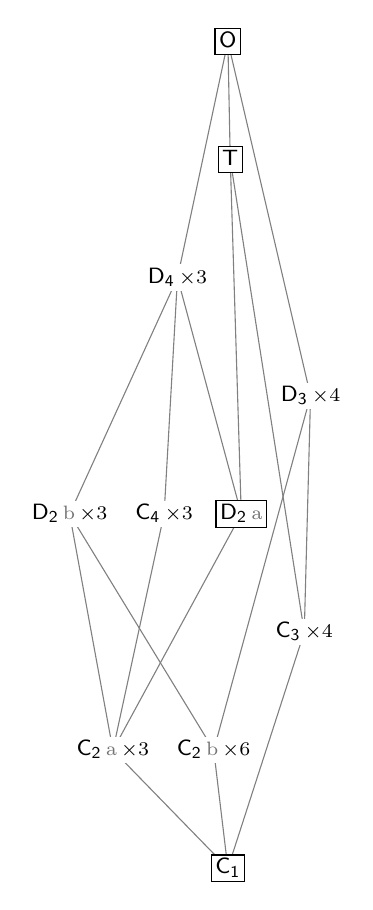
\begin{tikzpicture}[x=1cm, y=1.500cm,
  every node/.style={fill=white, font=\footnotesize, inner xsep=1.5pt, inner ysep=1.2pt, text height=5.6pt, text depth=1.6pt},
  normal/.style={draw, line width=0.4pt}, cover/.style={black!50, line width=0.4pt}]
\draw[cover] (0.00,0) -- (-1.46,1);
\draw[cover] (0.00,0) -- (-0.18,1);
\draw[cover] (0.00,0) -- (0.97,2);
\draw[cover] (-1.46,1) -- (-0.81,3);
\draw[cover] (-1.46,1) -- (0.17,3);
\draw[cover] (-1.46,1) -- (-2.01,3);
\draw[cover] (-0.18,1) -- (-2.01,3);
\draw[cover] (-0.18,1) -- (1.05,4);
\draw[cover] (0.97,2) -- (1.05,4);
\draw[cover] (0.97,2) -- (0.03,6);
\draw[cover] (-0.81,3) -- (-0.64,5);
\draw[cover] (0.17,3) -- (-0.64,5);
\draw[cover] (0.17,3) -- (0.03,6);
\draw[cover] (-2.01,3) -- (-0.64,5);
\draw[cover] (1.05,4) -- (0.00,7);
\draw[cover] (-0.64,5) -- (0.00,7);
\draw[cover] (0.03,6) -- (0.00,7);
\node[normal] (n00) at (0.00,0) {$\grp{C_{1}}$};
\node (n01) at (-1.46,1) {$\grp{C_{2}}$\clsletter{a}\,\nconj{3}};
\node (n02) at (-0.18,1) {$\grp{C_{2}}$\clsletter{b}\,\nconj{6}};
\node (n03) at (0.97,2) {$\grp{C_{3}}$\,\nconj{4}};
\node (n04) at (-0.81,3) {$\grp{C_{4}}$\,\nconj{3}};
\node[normal] (n05) at (0.17,3) {$\grp{D_{2}}$\clsletter{a}};
\node (n06) at (-2.01,3) {$\grp{D_{2}}$\clsletter{b}\,\nconj{3}};
\node (n07) at (1.05,4) {$\grp{D_{3}}$\,\nconj{4}};
\node (n08) at (-0.64,5) {$\grp{D_{4}}$\,\nconj{3}};
\node[normal] (n09) at (0.03,6) {$\grp{T}$};
\node[normal] (n10) at (0.00,7) {$\grp{O}$};
\end{tikzpicture}
\end{center}
{\small\setlength{\fillwidth}{\textwidth}\addtolength{\fillwidth}{-12\tabcolsep}\setlength{\colwidth}{0pt}\cellmax{$\grp{C_{2}}$\clsletter{a} $\samecls$ $\grp{D_{1}}$}\cellmax{$\grp{C_{2}}$\clsletter{b} $\samecls$ $\grp{D_{1}}$}\cellmax{subgrp}\cellmax{$\grp{D_{2}}$\clsletter{a}}\cellmax{$\grp{D_{2}}$\clsletter{b}}\cellmax{$\grp{C_{1}}$}\cellmax{$\grp{C_{3}}$}\cellmax{$\grp{C_{4}}$}\cellmax{$\grp{D_{3}}$}\cellmax{$\grp{D_{4}}$}\cellmax{$\grp{O}$}\cellmax{$\grp{T}$}\addtolength{\fillwidth}{-\colwidth}\setlength{\colwidth}{0pt}\cellmax{order}\cellmax{12}\cellmax{24}\cellmax{1}\cellmax{2}\cellmax{3}\cellmax{4}\cellmax{6}\cellmax{8}\addtolength{\fillwidth}{-\colwidth}\setlength{\colwidth}{0pt}\cellmax{conjugates}\cellmax{1}\cellmax{3}\cellmax{4}\cellmax{6}\addtolength{\fillwidth}{-\colwidth}\setlength{\colwidth}{0pt}\cellmax{normal}\cellmax{yes}\cellmax{no}\addtolength{\fillwidth}{-\colwidth}\setlength{\colwidth}{0pt}\cellmax{$\grp{N}_{\hairsp \grp{O}}(\grp{H})$}\cellmax{$\grp{D_{2}}$\clsletter{b}}\cellmax{$\grp{D_{3}}$}\cellmax{$\grp{D_{4}}$}\cellmax{$\grp{O}$}\addtolength{\fillwidth}{-\colwidth}\setlength{\colwidth}{0pt}\cellmax{$\grp{C}_{\hairsp \grp{O}}(\grp{H})$}\cellmax{$\grp{C_{2}}$\clsletter{a}}\cellmax{$\grp{D_{2}}$\clsletter{a}}\cellmax{$\grp{D_{2}}$\clsletter{b}}\cellmax{$\grp{C_{1}}$}\cellmax{$\grp{C_{3}}$}\cellmax{$\grp{C_{4}}$}\cellmax{$\grp{D_{4}}$}\cellmax{$\grp{O}$}\addtolength{\fillwidth}{-\colwidth}\setlength{\colwidth}{0pt}\cellmax{$\cls{6C_{4}}$, $\cls{3C_{2}}$, $\cls{6C_{2}}$}\cellmax{$\cls{3C_{2}}$, $\cls{6C_{2}}$}\cellmax{$\cls{6C_{4}}$, $\cls{3C_{2}}$}\cellmax{$\cls{8C_{3}}$, $\cls{3C_{2}}$}\cellmax{$\cls{8C_{3}}$, $\cls{6C_{2}}$}\cellmax{classes}\cellmax{$\cls{3C_{2}}$}\cellmax{$\cls{6C_{2}}$}\cellmax{$\cls{8C_{3}}$}\cellmax{---}\cellmax{all}\fillcap\begin{longtable}{@{}lrrlll>{\RaggedRight\arraybackslash}p{\fillwidth}@{}}\toprule
subgrp & order & conjugates & normal & $\grp{N}_{\hairsp \grp{O}}(\grp{H})$ & $\grp{C}_{\hairsp \grp{O}}(\grp{H})$ & classes\\\midrule\endhead
\bottomrule\endfoot\endlastfoot
\href{C1.pdf}{$\grp{C_{1}}$} & 1 & 1 & yes & \href{O.pdf}{$\grp{O}$} & \href{O.pdf}{$\grp{O}$} & ---\\*
\href{C2.pdf}{$\grp{C_{2}}$}\clsletter{a} $\samecls$ \href{D1.pdf}{$\grp{D_{1}}$} & 2 & 3 & no & \href{D4.pdf}{$\grp{D_{4}}$} & \href{D4.pdf}{$\grp{D_{4}}$} & $\cls{3C_{2}}$\\
\href{C2.pdf}{$\grp{C_{2}}$}\clsletter{b} $\samecls$ \href{D1.pdf}{$\grp{D_{1}}$} & 2 & 6 & no & \href{D2.pdf}{$\grp{D_{2}}$}\clsletter{b} & \href{D2.pdf}{$\grp{D_{2}}$}\clsletter{b} & $\cls{6C_{2}}$\\
\href{C3.pdf}{$\grp{C_{3}}$} & 3 & 4 & no & \href{D3.pdf}{$\grp{D_{3}}$} & \href{C3.pdf}{$\grp{C_{3}}$} & $\cls{8C_{3}}$\\
\href{C4.pdf}{$\grp{C_{4}}$} & 4 & 3 & no & \href{D4.pdf}{$\grp{D_{4}}$} & \href{C4.pdf}{$\grp{C_{4}}$} & $\cls{6C_{4}}$, $\cls{3C_{2}}$\\
\href{D2.pdf}{$\grp{D_{2}}$}\clsletter{a} & 4 & 1 & yes & \href{O.pdf}{$\grp{O}$} & \href{D2.pdf}{$\grp{D_{2}}$}\clsletter{a} & $\cls{3C_{2}}$\\
\href{D2.pdf}{$\grp{D_{2}}$}\clsletter{b} & 4 & 3 & no & \href{D4.pdf}{$\grp{D_{4}}$} & \href{D2.pdf}{$\grp{D_{2}}$}\clsletter{b} & $\cls{3C_{2}}$, $\cls{6C_{2}}$\\
\href{D3.pdf}{$\grp{D_{3}}$} & 6 & 4 & no & \href{D3.pdf}{$\grp{D_{3}}$} & \href{C1.pdf}{$\grp{C_{1}}$} & $\cls{8C_{3}}$, $\cls{6C_{2}}$\\
\href{D4.pdf}{$\grp{D_{4}}$} & 8 & 3 & no & \href{D4.pdf}{$\grp{D_{4}}$} & \href{C2.pdf}{$\grp{C_{2}}$}\clsletter{a} & $\cls{6C_{4}}$, $\cls{3C_{2}}$, $\cls{6C_{2}}$\\
\href{T.pdf}{$\grp{T}$} & 12 & 1 & yes & \href{O.pdf}{$\grp{O}$} & \href{C1.pdf}{$\grp{C_{1}}$} & $\cls{8C_{3}}$, $\cls{3C_{2}}$\\*
\href{O.pdf}{$\grp{O}$} & 24 & 1 & yes & \href{O.pdf}{$\grp{O}$} & \href{C1.pdf}{$\grp{C_{1}}$} & all\\
\bottomrule\end{longtable}}
\needspace{103pt}
\section{Descent of symmetry}\label{s:subduction}
Conventions: \href{../../CONVENTIONS.pdf}{CONVENTIONS.pdf}, sections \href{../../CONVENTIONS.pdf\#conv.12.2}{12.2} and \href{../../CONVENTIONS.pdf\#conv.12.4}{12.4}.
A column is a class of subgroups $\grp{H}$, in the order of the table of section~\ref{s:subgroups}, by its symbol in the row subgrp as there, with the letter that tells apart classes with the same symbol, which are not conjugate in $\grp{O}$; the symbol links to the document of $\grp{H}$. The entry of row $\Gamma$ is $\restr{\Gamma}{\grp{H}}$, the restriction of $\Gamma$ along a monomorphism from the record of $\grp{H}$ onto the subgroup, as a sum of the irreps of $\grp{H}$; the monomorphism identifies the subgroup with its record, and $\grp{H}$ names both. \label{n:group.normalizer.o3}\label{n:group.centralizer.o3}The record of $\grp{H}$ maps onto the subgroup in $\grpindex{\grp{N}}{\grp{C}}$ ways, $h \mapsto g h g^{-1}$ ($h \in \grp{H}$) for the $g \in \grp{O(3)}$ that carry $\grp{H}$ to it, $\grp{N}$ and $\grp{C}$ the normalizer and the centralizer of $\grp{H}$ in \href{O3.pdf}{$\grp{O(3)}$}; the row centralizer of section Names and structure of the document of $\grp{H}$ gives $\grp{C}$ and this index (the index in the row normalizer is $\grpindex{\grp{N}}{\grp{H}}$). Two maps related by a conjugation in $\grp{O}$ give the same restriction, so the maps fall into $\grpindex{\grp{N}}{\grp{C}}/\grpindex{\grp{N}_{\hairsp \grp{O}}}{\grp{C}_{\hairsp \grp{O}}}$ classes, $\grp{N}_{\hairsp \grp{O}}$ and $\grp{C}_{\hairsp \grp{O}}$ the normalizer and the centralizer of the subgroup in $\grp{O}$ (the table of section~\ref{s:subgroups}). \label{n:head.setting}A subgroup whose classes give different tables has one column per table, its settings: 1 for the stored monomorphism (\texttt{monomorphism}) and 2, 3, \dots{} for the \texttt{alternative\symbol{95}settings}, each with the images of the generators of $\grp{H}$ (\texttt{setting}). \label{n:head.images}\label{n:element.generator.index}The row images gives, under each setting, each generator of $\grp{H}$ whose image differs between the settings, in their order, by the symbol of its class (\href{../../CONVENTIONS.pdf}{CONVENTIONS.pdf}, section \href{../../CONVENTIONS.pdf\#conv.5.1}{5.1}), mapped to the class of $\grp{O}$ that holds its image; where two generators share a symbol, a superscript number in brackets gives the generator's index in the document of $\grp{H}$. \label{n:irrep.Delta}Each other column under a subgroup is column 1 with each irrep $\Lambda$ of $\grp{H}$ replaced by $\Lambda$ composed with one automorphism of $\grp{H}$ that a conjugation in \href{O3.pdf}{$\grp{O(3)}$} induces and none in $\grp{O}$ does (\href{../../CONVENTIONS.pdf}{CONVENTIONS.pdf}, section \href{../../CONVENTIONS.pdf\#conv.12.1}{12.1}).
{\small\begin{longtable}{@{}lccccc@{}}\toprule
subgrp & \href{C2.pdf}{$\grp{C_{2}}$}\clsletter{a} & \href{C2.pdf}{$\grp{C_{2}}$}\clsletter{b} & \href{C3.pdf}{$\grp{C_{3}}$} & \href{C4.pdf}{$\grp{C_{4}}$} & \href{D2.pdf}{$\grp{D_{2}}$}\clsletter{a}\\\midrule\endhead
\bottomrule\endfoot\endlastfoot
$\irr{a}_{1}$ & $\irr{a}$ & $\irr{a}$ & $\irr{a}$ & $\irr{a}$ & $\irr{a}$\\*
$\irr{a}_{2}$ & $\irr{a}$ & $\irr{b}$ & $\irr{a}$ & $\irr{b}$ & $\irr{a}$\\*
$\irr{e}$ & $2\,\irr{a}$ & $\irr{a}\oplus \irr{b}$ & $\conjpair{1}\irr{e}\oplus \conjpair{2}\irr{e}$ & $\irr{a}\oplus \irr{b}$ & $2\,\irr{a}$\\*
$\irr{t}_{1}$ & $\irr{a}\oplus 2\,\irr{b}$ & $\irr{a}\oplus 2\,\irr{b}$ & $\irr{a}\oplus \conjpair{1}\irr{e}\oplus \conjpair{2}\irr{e}$ & $\irr{a}\oplus \conjpair{1}\irr{e}\oplus \conjpair{2}\irr{e}$ & $\irr{b}_{1}\oplus \irr{b}_{2}\oplus \irr{b}_{3}$\\*
$\irr{t}_{2}$ & $\irr{a}\oplus 2\,\irr{b}$ & $2\,\irr{a}\oplus \irr{b}$ & $\irr{a}\oplus \conjpair{1}\irr{e}\oplus \conjpair{2}\irr{e}$ & $\irr{b}\oplus \conjpair{1}\irr{e}\oplus \conjpair{2}\irr{e}$ & $\irr{b}_{1}\oplus \irr{b}_{2}\oplus \irr{b}_{3}$\\
\bottomrule\end{longtable}}
{\small\begin{longtable}{@{}lccccccc@{}}\toprule
subgrp & \multicolumn{3}{c}{\href{D2.pdf}{$\grp{D_{2}}$}\clsletter{b}} & \href{D3.pdf}{$\grp{D_{3}}$} & \multicolumn{2}{c}{\href{D4.pdf}{$\grp{D_{4}}$}} & \href{T.pdf}{$\grp{T}$}\\\cmidrule(lr){2-4}\cmidrule(lr){6-7}
setting & 1 & 2 & 3 &  & 1 & 2 & \\
images & {\scriptsize\begin{tabular}[t]{@{}c@{}}$\cls{\genidx{C_{2}}{1}} \mapsto \cls{3C_{2}}$\\$\cls{\genidx{C_{2}}{2}} \mapsto \cls{6C_{2}}$\end{tabular}} & {\scriptsize\begin{tabular}[t]{@{}c@{}}$\cls{\genidx{C_{2}}{1}} \mapsto \cls{6C_{2}}$\\$\cls{\genidx{C_{2}}{2}} \mapsto \cls{3C_{2}}$\end{tabular}} & {\scriptsize\begin{tabular}[t]{@{}c@{}}$\cls{\genidx{C_{2}}{1}} \mapsto \cls{6C_{2}}$\\$\cls{\genidx{C_{2}}{2}} \mapsto \cls{6C_{2}}$\end{tabular}} &  & {\scriptsize $\cls{C_{2}} \mapsto \cls{3C_{2}}$} & {\scriptsize $\cls{C_{2}} \mapsto \cls{6C_{2}}$} & \\\midrule\endhead
\bottomrule\endfoot\endlastfoot
$\irr{a}_{1}$ & $\irr{a}$ & $\irr{a}$ & $\irr{a}$ & $\irr{a}_{1}$ & $\irr{a}_{1}$ & $\irr{a}_{1}$ & $\irr{a}$\\*
$\irr{a}_{2}$ & $\irr{b}_{1}$ & $\irr{b}_{3}$ & $\irr{b}_{2}$ & $\irr{a}_{2}$ & $\irr{b}_{1}$ & $\irr{b}_{2}$ & $\irr{a}$\\*
$\irr{e}$ & $\irr{a}\oplus \irr{b}_{1}$ & $\irr{a}\oplus \irr{b}_{3}$ & $\irr{a}\oplus \irr{b}_{2}$ & $\irr{e}$ & $\irr{a}_{1}\oplus \irr{b}_{1}$ & $\irr{a}_{1}\oplus \irr{b}_{2}$ & $\conjpair{1}\irr{e}\oplus \conjpair{2}\irr{e}$\\*
$\irr{t}_{1}$ & $\irr{b}_{1}\oplus \irr{b}_{2}\oplus \irr{b}_{3}$ & $\irr{b}_{1}\oplus \irr{b}_{2}\oplus \irr{b}_{3}$ & $\irr{b}_{1}\oplus \irr{b}_{2}\oplus \irr{b}_{3}$ & $\irr{a}_{2}\oplus \irr{e}$ & $\irr{a}_{2}\oplus \irr{e}$ & $\irr{a}_{2}\oplus \irr{e}$ & $\irr{t}$\\*
$\irr{t}_{2}$ & $\irr{a}\oplus \irr{b}_{2}\oplus \irr{b}_{3}$ & $\irr{a}\oplus \irr{b}_{1}\oplus \irr{b}_{2}$ & $\irr{a}\oplus \irr{b}_{1}\oplus \irr{b}_{3}$ & $\irr{a}_{1}\oplus \irr{e}$ & $\irr{b}_{2}\oplus \irr{e}$ & $\irr{b}_{1}\oplus \irr{e}$ & $\irr{t}$\\
\bottomrule\end{longtable}}
Read down a column, a table gives induction (Frobenius reciprocity): $\Gamma$ occurs in $\Ind{\grp{H}}{\grp{O}} \Lambda$ as often as $\Lambda$ occurs in the entry of row $\Gamma$. The JSON gives, for every entry, the unitary matrix that carries $\restr{\Gamma}{\grp{H}}$ into the direct sum of the matrices of $\grp{H}$ (\texttt{subduction[].blocks}), and for every class the left coset representatives of $\grp{H}$ (\texttt{transversal}), from which \href{../../CONVENTIONS.pdf}{CONVENTIONS.pdf}, section \href{../../CONVENTIONS.pdf\#conv.12.4}{12.4}, builds $\Ind{\grp{H}}{\grp{O}} \Lambda$ and its intertwiners.
\needspace{171pt}
\partbox{Permutation representations}
\section{Figures}\label{s:permutation}
Conventions: \href{../../CONVENTIONS.pdf}{CONVENTIONS.pdf}, sections \href{../../CONVENTIONS.pdf\#conv.12.4}{12.4} to \href{../../CONVENTIONS.pdf\#conv.12.6}{12.6}.
\leavevmode\label{n:local.orbit.size}\label{n:local.matrix.permutation}Every class of subgroups $\grp{H}$ is the stabilizer of a figure in space, the subgroup of the elements that carry it into itself, and $\grp{O}$ permutes the $N = [\grp{O} : \grp{H}]$ copies of the figure as it permutes the right cosets $\grp{H}\xi_j$, $j = 0, 1, \dots, N - 1$, $\xi_j$ the element of least index of its coset, in the order of these indices ($\xi_0 = \cls{E}$): the copy $j$ is the figure moved by $\xi_j$. The element $g$ moves the copy $j$ to the copy $j'$, where $\grp{H}\xi_j g = \grp{H}\xi_{j'}$, and the permutation matrix $D(g)$, whose row $j$ has its one nonzero entry in column $j'$,
\begin{equation}\label{e:perm.matrix}\pointr_j\, P(g) = \pointr_{j'}, \qquad D(g)_{j,j'} = 1,\end{equation}
obeys $D(g)\, D(h) = D(gh)$. The copies are generated by the defining representation of $\grp{O}$, its matrices $P(g)$ (section~\ref{s:elements}), acting on the figure and its root point $\pointr_0$: $\pointr_j = \pointr_0\, P(\xi_j)$ is the point of the copy $j$ that $\pointr_0$ moves to. The JSON record stores the coordinates of the points of every copy, the images $j'$ of every copy under every element and the table of marks (\href{../../CONVENTIONS.pdf}{CONVENTIONS.pdf}, sections \href{../../CONVENTIONS.pdf\#conv.12.5}{12.5} and \href{../../CONVENTIONS.pdf\#conv.12.6}{12.6}).
\leavevmode\label{n:head.figure}\label{n:head.site}\label{n:head.vertices}\label{n:head.rank}\label{n:head.cos}\label{n:head.hand}The figure of a class is the first of these whose stabilizer is $\grp{H}$: the root point $\pointr_0$; the line through the origin along $\pointr_0$; a spin, the axial vector $\pointr_0$, a sense of rotation about that line; a spinning arrow, the arrow $\pointr_0$ with a sense of rotation about itself; a helix, the line along $\pointr_0$ with a handedness (these two only when $\grp{H}$ has no improper element and $\grp{O}$ has one); and otherwise the least orbit of $\pointr_0$ under $\grp{H}$ whose stabilizer is $\grp{H}$, a segment, a polygon or a polyhedron. The table has a row per class of subgroups, in the order of the table of section~\ref{s:subgroups} and named as there: $N$; the figure, by its shape or its number of points; site, the stabilizer of the point $\pointr_0$, which tells the symmetry elements of $\grp{O}$ that the figure lies on; $\pointr_0$; vertices, what the points of all the copies form (the tips of the arrows and spins, both ends of the lines and helices), with ${\times}k$ when $k > 1$ copies pass through each; rank, the number of classes of pairs of copies under $\grp{O}$, a copy with itself one of them; cos, for a point, a line or a spin of rank at most 5, the cosine of the angle between two copies, one per class of pairs other than a copy with itself (of the acute angle, for lines); and hand, 2 when $\grp{H}$ has no improper element and $\grp{O}$ has one, so that the rotations of $\grp{O}$ leave the copies in two classes, mirror images of each other: the left- and the right-handed copies of a chiral figure.
{\small\setlength{\tabcolsep}{4pt}\setlength{\fillwidth}{\textwidth}\addtolength{\fillwidth}{-16\tabcolsep}\setlength{\colwidth}{0pt}\cellmax{subgrp}\cellmax{$\grp{C_{2}}$\clsletter{a}}\cellmax{$\grp{C_{2}}$\clsletter{b}}\cellmax{$\grp{D_{2}}$\clsletter{a}}\cellmax{$\grp{D_{2}}$\clsletter{b}}\cellmax{$\grp{C_{1}}$}\cellmax{$\grp{C_{3}}$}\cellmax{$\grp{C_{4}}$}\cellmax{$\grp{D_{3}}$}\cellmax{$\grp{D_{4}}$}\cellmax{$\grp{O}$}\cellmax{$\grp{T}$}\addtolength{\fillwidth}{-\colwidth}\setlength{\colwidth}{0pt}\cellmax{12}\cellmax{24}\cellmax{$N$}\cellmax{1}\cellmax{2}\cellmax{3}\cellmax{4}\cellmax{6}\cellmax{8}\addtolength{\fillwidth}{-\colwidth}\setlength{\colwidth}{0pt}\cellmax{tetrahedron}\cellmax{rectangle}\cellmax{figure}\cellmax{origin}\cellmax{point}\cellmax{line}\addtolength{\fillwidth}{-\colwidth}\setlength{\colwidth}{0pt}\cellmax{$\grp{C_{2}}$\clsletter{b}}\cellmax{site}\cellmax{$\grp{C_{1}}$}\cellmax{$\grp{C_{3}}$}\cellmax{$\grp{C_{4}}$}\cellmax{$\grp{O}$}\addtolength{\fillwidth}{-\colwidth}\setlength{\colwidth}{0pt}\cellmax{$(-1, -1, 1)$}\cellmax{$(-1, 0, 1)$}\cellmax{$(1, -1, 0)$}\cellmax{$(1, 1, -1)$}\cellmax{$(0, 0, 0)$}\cellmax{$(0, 0, 1)$}\cellmax{$(1, 2, 0)$}\cellmax{$(1, 2, 4)$}\cellmax{$\pointr_0$}\addtolength{\fillwidth}{-\colwidth}\setlength{\colwidth}{0pt}\cellmax{cuboctahedron}\cellmax{octahedron}\cellmax{24 points}\cellmax{vertices}\cellmax{origin}\cellmax{cube}\addtolength{\fillwidth}{-\colwidth}\setlength{\colwidth}{0pt}\cellmax{rank}\cellmax{24}\cellmax{1}\cellmax{2}\cellmax{3}\cellmax{4}\cellmax{6}\cellmax{7}\cellmax{8}\addtolength{\fillwidth}{-\colwidth}\setlength{\colwidth}{0pt}\cellmax{hand}\cellmax{}\addtolength{\fillwidth}{-\colwidth}\setlength{\colwidth}{0pt}\cellmax{${\tfrac{1}{3}}$, ${-\tfrac{1}{3}}$, ${-1}$}\cellmax{${0}$, ${-1}$}\cellmax{${0}$, ${\tfrac{1}{2}}$}\cellmax{cos}\cellmax{${0}$}\cellmax{${\tfrac{1}{3}}$}\fillcap{\renewcommand{\arraystretch}{1.3}\begin{longtable}{@{}lrllllr>{\RaggedRight\arraybackslash}p{\fillwidth}r@{}}\toprule
subgrp & $N$ & figure & site & $\pointr_0$ & vertices & rank & cos & hand\\\midrule\endhead
\bottomrule\endfoot\endlastfoot
\href{C1.pdf}{$\grp{C_{1}}$} & 24 & point & \href{C1.pdf}{$\grp{C_{1}}$} & $(1, 2, 4)$ & 24 points & 24 &  & \\*
\href{C2.pdf}{$\grp{C_{2}}$}\clsletter{a} & 12 & line & \href{C1.pdf}{$\grp{C_{1}}$} & $(1, 2, 0)$ & 24 points & 8 &  & \\
\href{C2.pdf}{$\grp{C_{2}}$}\clsletter{b} & 12 & point & \href{C2.pdf}{$\grp{C_{2}}$}\clsletter{b} & $(-1, 0, 1)$ & cuboctahedron & 7 &  & \\
\href{C3.pdf}{$\grp{C_{3}}$} & 8 & point & \href{C3.pdf}{$\grp{C_{3}}$} & $(-1, -1, 1)$ & cube & 4 & ${\tfrac{1}{3}}$, ${-\tfrac{1}{3}}$, ${-1}$ & \\
\href{C4.pdf}{$\grp{C_{4}}$} & 6 & point & \href{C4.pdf}{$\grp{C_{4}}$} & $(0, 0, 1)$ & octahedron & 3 & ${0}$, ${-1}$ & \\
\href{D2.pdf}{$\grp{D_{2}}$}\clsletter{a} & 6 & rectangle & \href{C1.pdf}{$\grp{C_{1}}$} & $(1, 2, 0)$ & 24 points & 6 &  & \\
\href{D2.pdf}{$\grp{D_{2}}$}\clsletter{b} & 6 & line & \href{C2.pdf}{$\grp{C_{2}}$}\clsletter{b} & $(1, -1, 0)$ & cuboctahedron & 3 & ${0}$, ${\tfrac{1}{2}}$ & \\
\href{D3.pdf}{$\grp{D_{3}}$} & 4 & line & \href{C3.pdf}{$\grp{C_{3}}$} & $(1, 1, -1)$ & cube & 2 & ${\tfrac{1}{3}}$ & \\
\href{D4.pdf}{$\grp{D_{4}}$} & 3 & line & \href{C4.pdf}{$\grp{C_{4}}$} & $(0, 0, 1)$ & octahedron & 2 & ${0}$ & \\
\href{T.pdf}{$\grp{T}$} & 2 & tetrahedron & \href{C3.pdf}{$\grp{C_{3}}$} & $(-1, -1, 1)$ & cube & 2 &  & \\*
\href{O.pdf}{$\grp{O}$} & 1 & origin & \href{O.pdf}{$\grp{O}$} & $(0, 0, 0)$ & origin & 1 &  & \\
\bottomrule\end{longtable}}}
The copies of the figure of \href{T.pdf}{$\grp{T}$} form the compound of two tetrahedra (UC04), numbered as in the list of the uniform compounds [\href{../../../REFERENCES.pdf\#ref.Ski76}{Ski76}]. Some points give an orbit that is a uniform polyhedron, with regular faces and all its vertices alike, or a regular polygon: for \href{C1.pdf}{$\grp{C_{1}}$}, a truncated cube, a truncated octahedron, a rhombicuboctahedron or a snub cube.
\needspace{153pt}
\section{Decompositions}\label{s:decompositions}
Conventions: \href{../../CONVENTIONS.pdf}{CONVENTIONS.pdf}, sections \href{../../CONVENTIONS.pdf\#conv.12.4}{12.4} and \href{../../CONVENTIONS.pdf\#conv.12.5}{12.5}.
The kernel of the permutation representation of a class is the subgroup of the elements that leave every copy in place, and the decomposition is that of $D$, whose character at $g$ is the number of copies that $g$ leaves in place: an irrep occurs in $D$ as often as the trivial irrep of $\grp{H}$ occurs in its restriction to $\grp{H}$ (section~\ref{s:subduction}).
{\small\medmuskip=4mu plus 2mu\relax\setlength{\fillwidth}{\textwidth}\addtolength{\fillwidth}{-6\tabcolsep}\setlength{\colwidth}{0pt}\cellmax{subgrp}\cellmax{$\grp{C_{2}}$\clsletter{a}}\cellmax{$\grp{C_{2}}$\clsletter{b}}\cellmax{$\grp{D_{2}}$\clsletter{a}}\cellmax{$\grp{D_{2}}$\clsletter{b}}\cellmax{$\grp{C_{1}}$}\cellmax{$\grp{C_{3}}$}\cellmax{$\grp{C_{4}}$}\cellmax{$\grp{D_{3}}$}\cellmax{$\grp{D_{4}}$}\cellmax{$\grp{O}$}\cellmax{$\grp{T}$}\addtolength{\fillwidth}{-\colwidth}\setlength{\colwidth}{0pt}\cellmax{12}\cellmax{24}\cellmax{$N$}\cellmax{1}\cellmax{2}\cellmax{3}\cellmax{4}\cellmax{6}\cellmax{8}\addtolength{\fillwidth}{-\colwidth}\setlength{\colwidth}{0pt}\cellmax{kernel}\cellmax{$\grp{D_{2}}$\clsletter{a}}\cellmax{$\grp{C_{1}}$}\cellmax{$\grp{O}$}\cellmax{$\grp{T}$}\addtolength{\fillwidth}{-\colwidth}\setlength{\colwidth}{0pt}\cellmax{$\irr{a}_{1}\oplus \irr{a}_{2}\oplus 2\,\irr{e}\oplus 3\,\irr{t}_{1}\oplus 3\,\irr{t}_{2}$}\cellmax{$\irr{a}_{1}\oplus \irr{a}_{2}\oplus 2\,\irr{e}\oplus \irr{t}_{1}\oplus \irr{t}_{2}$}\cellmax{$\irr{a}_{1}\oplus \irr{a}_{2}\oplus \irr{t}_{1}\oplus \irr{t}_{2}$}\cellmax{$\irr{a}_{1}\oplus \irr{e}\oplus \irr{t}_{1}\oplus 2\,\irr{t}_{2}$}\cellmax{decomposition}\cellmax{$\irr{a}_{1}\oplus \irr{a}_{2}\oplus 2\,\irr{e}$}\cellmax{$\irr{a}_{1}\oplus \irr{e}\oplus \irr{t}_{1}$}\cellmax{$\irr{a}_{1}\oplus \irr{e}\oplus \irr{t}_{2}$}\cellmax{$\irr{a}_{1}\oplus \irr{a}_{2}$}\cellmax{$\irr{a}_{1}\oplus \irr{t}_{2}$}\cellmax{$\irr{a}_{1}\oplus \irr{e}$}\cellmax{$\irr{a}_{1}$}\fillcap\begin{longtable}{@{}lrl>{\RaggedRight\arraybackslash}p{\fillwidth}@{}}\toprule
subgrp & $N$ & kernel & decomposition\\\midrule\endhead
\bottomrule\endfoot\endlastfoot
\href{C1.pdf}{$\grp{C_{1}}$} & 24 & \href{C1.pdf}{$\grp{C_{1}}$} & $\irr{a}_{1}\oplus \irr{a}_{2}\oplus 2\,\irr{e}\oplus 3\,\irr{t}_{1}\oplus 3\,\irr{t}_{2}$\\*
\href{C2.pdf}{$\grp{C_{2}}$}\clsletter{a} & 12 & \href{C1.pdf}{$\grp{C_{1}}$} & $\irr{a}_{1}\oplus \irr{a}_{2}\oplus 2\,\irr{e}\oplus \irr{t}_{1}\oplus \irr{t}_{2}$\\
\href{C2.pdf}{$\grp{C_{2}}$}\clsletter{b} & 12 & \href{C1.pdf}{$\grp{C_{1}}$} & $\irr{a}_{1}\oplus \irr{e}\oplus \irr{t}_{1}\oplus 2\,\irr{t}_{2}$\\
\href{C3.pdf}{$\grp{C_{3}}$} & 8 & \href{C1.pdf}{$\grp{C_{1}}$} & $\irr{a}_{1}\oplus \irr{a}_{2}\oplus \irr{t}_{1}\oplus \irr{t}_{2}$\\
\href{C4.pdf}{$\grp{C_{4}}$} & 6 & \href{C1.pdf}{$\grp{C_{1}}$} & $\irr{a}_{1}\oplus \irr{e}\oplus \irr{t}_{1}$\\
\href{D2.pdf}{$\grp{D_{2}}$}\clsletter{a} & 6 & \href{D2.pdf}{$\grp{D_{2}}$}\clsletter{a} & $\irr{a}_{1}\oplus \irr{a}_{2}\oplus 2\,\irr{e}$\\
\href{D2.pdf}{$\grp{D_{2}}$}\clsletter{b} & 6 & \href{C1.pdf}{$\grp{C_{1}}$} & $\irr{a}_{1}\oplus \irr{e}\oplus \irr{t}_{2}$\\
\href{D3.pdf}{$\grp{D_{3}}$} & 4 & \href{C1.pdf}{$\grp{C_{1}}$} & $\irr{a}_{1}\oplus \irr{t}_{2}$\\
\href{D4.pdf}{$\grp{D_{4}}$} & 3 & \href{D2.pdf}{$\grp{D_{2}}$}\clsletter{a} & $\irr{a}_{1}\oplus \irr{e}$\\
\href{T.pdf}{$\grp{T}$} & 2 & \href{T.pdf}{$\grp{T}$} & $\irr{a}_{1}\oplus \irr{a}_{2}$\\*
\href{O.pdf}{$\grp{O}$} & 1 & \href{O.pdf}{$\grp{O}$} & $\irr{a}_{1}$\\
\bottomrule\end{longtable}}
\needspace{103pt}
\section{Cycle types}\label{s:cycle_types}
Conventions: \href{../../CONVENTIONS.pdf}{CONVENTIONS.pdf}, section \href{../../CONVENTIONS.pdf\#conv.12.5}{12.5}.
\leavevmode\label{n:local.cycle.type}\label{n:local.cycle.length}\label{n:local.cycle.count}\label{n:local.cycles}\label{n:local.states}The entry in the row of a class of subgroups and the column of a class of elements is the cycle type of $j \mapsto j'$ for the elements of the class, $\ell^{c}$ for $c$ cycles of length $\ell$. The cycles of length 1 are the copies that the element leaves in place, whose number is the character of $D$; with $c(g)$ cycles in all, $g$ has the character $q^{c(g)}$ on the $q^N$ products of one of $q$ states of each copy (\href{../../CONVENTIONS.pdf}{CONVENTIONS.pdf}, section \href{../../CONVENTIONS.pdf\#conv.12.5}{12.5}).
{\small\setlength{\tabcolsep}{4pt}\begin{longtable}{@{}lrccccc@{}}\toprule
subgrp & $N$ & $\cls{E}$ & $\cls{6C_{4}}$ & $\cls{8C_{3}}$ & $\cls{3C_{2}}$ & $\cls{6C_{2}}$\\\midrule\endhead
\bottomrule\endfoot\endlastfoot
\href{C1.pdf}{$\grp{C_{1}}$} & 24 & $1^{24}$ & $4^{6}$ & $3^{8}$ & $2^{12}$ & $2^{12}$\\*
\href{C2.pdf}{$\grp{C_{2}}$}\clsletter{a} & 12 & $1^{12}$ & $2^{2}\,4^{2}$ & $3^{4}$ & $1^{4}\,2^{4}$ & $2^{6}$\\*
\href{C2.pdf}{$\grp{C_{2}}$}\clsletter{b} & 12 & $1^{12}$ & $4^{3}$ & $3^{4}$ & $2^{6}$ & $1^{2}\,2^{5}$\\*
\href{C3.pdf}{$\grp{C_{3}}$} & 8 & $1^{8}$ & $4^{2}$ & $1^{2}\,3^{2}$ & $2^{4}$ & $2^{4}$\\*
\href{C4.pdf}{$\grp{C_{4}}$} & 6 & $1^{6}$ & $1^{2}\,4$ & $3^{2}$ & $1^{2}\,2^{2}$ & $2^{3}$\\*
\href{D2.pdf}{$\grp{D_{2}}$}\clsletter{a} & 6 & $1^{6}$ & $2^{3}$ & $3^{2}$ & $1^{6}$ & $2^{3}$\\*
\href{D2.pdf}{$\grp{D_{2}}$}\clsletter{b} & 6 & $1^{6}$ & $2\,4$ & $3^{2}$ & $1^{2}\,2^{2}$ & $1^{2}\,2^{2}$\\*
\href{D3.pdf}{$\grp{D_{3}}$} & 4 & $1^{4}$ & $4$ & $1\,3$ & $2^{2}$ & $1^{2}\,2$\\*
\href{D4.pdf}{$\grp{D_{4}}$} & 3 & $1^{3}$ & $1\,2$ & $3$ & $1^{3}$ & $1\,2$\\*
\href{T.pdf}{$\grp{T}$} & 2 & $1^{2}$ & $2$ & $1^{2}$ & $1^{2}$ & $2$\\
\bottomrule\end{longtable}}
\needspace{177pt}
\partbox{Angular momentum}
\section{Subduction from \texorpdfstring{$\grp{O(3)}$}{O(3)}}\label{s:subduction_o3}
Conventions: \href{../../CONVENTIONS.pdf}{CONVENTIONS.pdf}, section \href{../../CONVENTIONS.pdf\#conv.11}{11}.
\leavevmode\label{n:index.J}\label{n:index.parity}\label{n:function.multiplicity}$\irrJp{J}{p}$ is the irrep of \href{O3.pdf}{$\grp{O(3)}$} of angular momentum $J$ and parity $p$ ($p = +1$: $\ptag{g}$, $p = -1$: $\ptag{u}$), and $b_\Gamma(J, p)$ the multiplicity of $\Gamma$ in
\begin{equation}\label{e:o3}\restr{\irrJp{J}{p}}{\grp{O}} .\end{equation}
\leavevmode\label{n:index.increment}Each table gives $b_\Gamma(J, p)$ for $J \le 20$, and $b_\Gamma(J + 12, p) = b_\Gamma(J, p) + \Delta_\Gamma$ for every $J$, $\Delta_\Gamma$ the last row of the table of parity $p$. The multiplicities do not depend on $p$, as every element of $\grp{O}$ is a rotation: one table holds both parities.
\needspace{218pt}
\paragraph{Parity $\ptag{g}$ and $\ptag{u}$ ($p = \pm1$).}
{\small\begin{longtable}{@{}rrrrrr@{\hspace{18pt}}rrrrrr@{}}\toprule
$J$ & $\irr{a}_{1}$ & $\irr{a}_{2}$ & $\irr{e}$ & $\irr{t}_{1}$ & $\irr{t}_{2}$ & $J$ & $\irr{a}_{1}$ & $\irr{a}_{2}$ & $\irr{e}$ & $\irr{t}_{1}$ & $\irr{t}_{2}$\\\midrule\endhead
\bottomrule\endfoot\endlastfoot
0 & 1 & 0 & 0 & 0 & 0 & 11 & 0 & 1 & 2 & 3 & 3\\*
1 & 0 & 0 & 0 & 1 & 0 & 12 & 2 & 1 & 2 & 3 & 3\\*
2 & 0 & 0 & 1 & 0 & 1 & 13 & 1 & 1 & 2 & 4 & 3\\*
3 & 0 & 1 & 0 & 1 & 1 & 14 & 1 & 1 & 3 & 3 & 4\\*
4 & 1 & 0 & 1 & 1 & 1 & 15 & 1 & 2 & 2 & 4 & 4\\*
5 & 0 & 0 & 1 & 2 & 1 & 16 & 2 & 1 & 3 & 4 & 4\\*
6 & 1 & 1 & 1 & 1 & 2 & 17 & 1 & 1 & 3 & 5 & 4\\*
7 & 0 & 1 & 1 & 2 & 2 & 18 & 2 & 2 & 3 & 4 & 5\\*
8 & 1 & 0 & 2 & 2 & 2 & 19 & 1 & 2 & 3 & 5 & 5\\*
9 & 1 & 1 & 1 & 3 & 2 & 20 & 2 & 1 & 4 & 5 & 5\\*\noalign{\vskip 1.5pt}\multispan{6} & \multispan{6}\leaders\hrule height\cmidrulewidth\hfill\kern0pt\\*\noalign{\vskip 1.5pt}
10 & 1 & 1 & 2 & 2 & 3 & $\Delta_\Gamma$ & 1 & 1 & 2 & 3 & 3\\
\bottomrule\end{longtable}}
\needspace{110pt}
\section{Multiplicities and allowed \texorpdfstring{$m$}{m}}\label{s:multiplicities}
Conventions: \href{../../CONVENTIONS.pdf}{CONVENTIONS.pdf}, section \href{../../CONVENTIONS.pdf\#conv.14}{14}.
\leavevmode\label{n:function.generating}\label{n:index.generating.variable}$b_\Gamma(J) = b_\Gamma(J, (-1)^J)$, the number of blocks of $\Gamma$ at $J$, and
\begin{equation}\label{e:gf}H_\Gamma(t) = \sum_{J\ge0} b_\Gamma(J)\,t^J,\end{equation}
\leavevmode\label{n:function.generating.numerator}its generating function, $H_\Gamma(t) = P_\Gamma(t)/((1-t^{4})(1-t^{6}))$. \label{n:head.parity}Every nonzero component of a vector of $\Gamma$ has $m \bmod 4$ in the listed residues, and each listed residue occurs; a dash: no block of $\Gamma$ at that parity of $J$.
{\small\begin{longtable}{@{}llll@{}}\toprule
$\Gamma$ & $P_\Gamma(t)$ & $m \bmod 4$, $J$ even & $J$ odd\\\midrule\endhead
\bottomrule\endfoot\endlastfoot
$\irr{a}_{1}$ & $1 + t^{9}$ & 0 & 0\\*
$\irr{a}_{2}$ & $t^{3} + t^{6}$ & 2 & 2\\*
$\irr{e}$ & $t^{2} + t^{4} + t^{5} + t^{7}$ & 0, 2 & 0, 2\\*
$\irr{t}_{1}$ & $t + t^{3} + t^{4} + t^{5} + t^{6} + t^{8}$ & 0, 1, 3 & 0, 1, 3\\*
$\irr{t}_{2}$ & $t^{2} + t^{3} + t^{4} + t^{5} + t^{6} + t^{7}$ & 1, 2, 3 & 1, 2, 3\\
\bottomrule\end{longtable}}
\needspace{110pt}
\section{Symmetry-adapted bases}\label{s:bases}
Conventions: \href{../../CONVENTIONS.pdf}{CONVENTIONS.pdf}, sections \href{../../CONVENTIONS.pdf\#conv.14}{14}, \href{../../CONVENTIONS.pdf\#conv.14.2}{14.2} to \href{../../CONVENTIONS.pdf\#conv.14.4}{14.4}.
\leavevmode\label{n:index.m}\label{n:vector.ket}\label{n:index.ketcoefficient}\label{n:vector.basis.symmetry}\label{n:index.ketweight}\label{n:index.total}The kets $\jm{J}{m}$ are the spherical harmonics (the inversion acts as $(-1)^J$), and a vector is listed by its coefficients $e_m$:
\begin{equation}\label{e:ket}v = \frac{1}{\sqrt{\mathrm{tot}}}\sum_m e_m\sqrt{F_m}\;\jm{J}{m},\qquad F_m = (J+m)!\,(J-m)!,\qquad \mathrm{tot} = \sum_m |e_m|^2F_m,\end{equation}
\leavevmode\label{n:index.factor.c}\label{n:index.multiplicity.copies}the amplitude of $\jm{J}{m}$ being $e_m\sqrt{F_m/\mathrm{tot}}$; a vector written $c\sum_m q_m\jm{J}{m}$ has $e_m = c\,q_m$.
\leavevmode\label{n:matrix.projector}The copies of $\Gamma$ at $J$ are orthonormal. Their partner-1 vectors are the vectors of the reduced row echelon basis, in the coordinates $e_m$, $m = -J, -J+1, \dots, J$, of the range of
\begin{equation}\label{e:projector}P^\Gamma_{1,1} = \sum_g \conj{\repD{\Gamma}_{1,1}(g)}\,\irrJ{J}(g),\end{equation}
$\mult$ ascending with the lowest $m$ of each, each less its projections on the copies before it (Gram--Schmidt); partner $\intx$ is $P^\Gamma_{\intx,1}$ applied to partner 1. The files hold $J = 0, 1, \dots, 60$: $J \le 10$ in the repository, $J = 11, 12, \dots, 60$ in its release (README.md).
\label{n:head.vector}51 blocks, 121 vectors, $J = 0, 1, \dots, 10$; a row gives a vector of a block at $J$: the block's irrep and copy index $\mult$, the partner index $\intx$ and the vector; the full set $J = 0, 1, \dots, 60$ (1551 blocks, 3721 vectors) is in \texttt{data/symmetry\symbol{95}adapted\symbol{95}bases/O/}, $J \le 10$ in the repository and $J = 11, 12, \dots, 60$ in the release archive \texttt{O\symbol{95}J011-J060.tar}, which unpacks in the folder \texttt{rotation/} (README.md).
{\small\setlength{\tabcolsep}{3pt}\setlength{\fillwidth}{\textwidth}\addtolength{\fillwidth}{-\dimexpr 6\tabcolsep+4pt\relax}\setlength{\colwidth}{0pt}\cellmax{10}\cellmax{$J$}\cellmax{0}\cellmax{1}\cellmax{2}\cellmax{3}\cellmax{4}\cellmax{5}\cellmax{6}\cellmax{7}\cellmax{8}\cellmax{9}\addtolength{\fillwidth}{-\colwidth}\setlength{\colwidth}{0pt}\cellmax{irrep}\cellmax{$\irr{a}_{1}$}\cellmax{$\irr{a}_{2}$}\cellmax{$\irr{t}_{1}$}\cellmax{$\irr{t}_{2}$}\cellmax{$\irr{e}$}\addtolength{\fillwidth}{-\colwidth}\setlength{\colwidth}{0pt}\cellmax{$\mult$}\cellmax{1}\cellmax{2}\cellmax{3}\addtolength{\fillwidth}{-\colwidth}\setlength{\colwidth}{0pt}\cellmax{$\intx$}\cellmax{1}\cellmax{2}\cellmax{3}\addtolength{\fillwidth}{-\colwidth}\setlength{\colwidth}{0pt}\cellmax{$-\iunit\sqrt{3}\,\jm{10}{-10}$ $+$ $394\,\jm{10}{-8}$ $-$ $1581\iunit\sqrt{3}\,\jm{10}{-6}$ $-$ $4488\,\jm{10}{-4}$ $+$ $1326\iunit\sqrt{3}\,\jm{10}{-2}$ $+$ $9724\,\jm{10}{0}$ $+$ $1326\iunit\sqrt{3}\,\jm{10}{2}$ $-$ $4488\,\jm{10}{4}$ $-$ $1581\iunit\sqrt{3}\,\jm{10}{6}$ $+$ $394\,\jm{10}{8}$ $-$ $\iunit\sqrt{3}\,\jm{10}{10}$}\cellmax{$\iunit\sqrt{3}\,\jm{10}{-10}$ $+$ $394\,\jm{10}{-8}$ $+$ $1581\iunit\sqrt{3}\,\jm{10}{-6}$ $-$ $4488\,\jm{10}{-4}$ $-$ $1326\iunit\sqrt{3}\,\jm{10}{-2}$ $+$ $9724\,\jm{10}{0}$ $-$ $1326\iunit\sqrt{3}\,\jm{10}{2}$ $-$ $4488\,\jm{10}{4}$ $+$ $1581\iunit\sqrt{3}\,\jm{10}{6}$ $+$ $394\,\jm{10}{8}$ $+$ $\iunit\sqrt{3}\,\jm{10}{10}$}\cellmax{$\iunit{}\,(7\,\jm{10}{-9}$ $-$ $95\,\jm{10}{-7}$ $+$ $476\,\jm{10}{-5}$ $-$ $748\,\jm{10}{-3}$ $-$ $1326\,\jm{10}{-1}$ $+$ $1326\,\jm{10}{1}$ $+$ $748\,\jm{10}{3}$ $-$ $476\,\jm{10}{5}$ $+$ $95\,\jm{10}{7}$ $-$ $7\,\jm{10}{9})$}\cellmax{$-\iunit{}\,(5\,\jm{10}{-9}$ $+$ $35\,\jm{10}{-7}$ $+$ $132\,\jm{10}{-5}$ $-$ $20\,\jm{10}{-3}$ $+$ $390\,\jm{10}{-1}$ $-$ $390\,\jm{10}{1}$ $+$ $20\,\jm{10}{3}$ $-$ $132\,\jm{10}{5}$ $-$ $35\,\jm{10}{7}$ $-$ $5\,\jm{10}{9})$}\cellmax{$7\,\jm{10}{-9}$ $+$ $95\,\jm{10}{-7}$ $+$ $476\,\jm{10}{-5}$ $+$ $748\,\jm{10}{-3}$ $-$ $1326\,\jm{10}{-1}$ $-$ $1326\,\jm{10}{1}$ $+$ $748\,\jm{10}{3}$ $+$ $476\,\jm{10}{5}$ $+$ $95\,\jm{10}{7}$ $+$ $7\,\jm{10}{9}$}\cellmax{$-\iunit{}\,(91\,\jm{10}{-9}$ $-$ $2399\,\jm{10}{-7}$ $+$ $5576\,\jm{10}{-3}$ $+$ $22542\,\jm{10}{-1}$ $-$ $22542\,\jm{10}{1}$ $-$ $5576\,\jm{10}{3}$ $+$ $2399\,\jm{10}{7}$ $-$ $91\,\jm{10}{9})$}\cellmax{$-\iunit{}\,(\jm{9}{-9}$ $-$ $167\,\jm{9}{-7}$ $+$ $820\,\jm{9}{-5}$ $+$ $1092\,\jm{9}{-3}$ $-$ $2002\,\jm{9}{-1}$ $-$ $2002\,\jm{9}{1}$ $+$ $1092\,\jm{9}{3}$ $+$ $820\,\jm{9}{5}$ $-$ $167\,\jm{9}{7}$ $+$ $\jm{9}{9})$}\cellmax{$5\,\jm{10}{-9}$ $-$ $35\,\jm{10}{-7}$ $+$ $132\,\jm{10}{-5}$ $+$ $20\,\jm{10}{-3}$ $+$ $390\,\jm{10}{-1}$ $+$ $390\,\jm{10}{1}$ $+$ $20\,\jm{10}{3}$ $+$ $132\,\jm{10}{5}$ $-$ $35\,\jm{10}{7}$ $+$ $5\,\jm{10}{9}$}\cellmax{$-\jm{10}{-10}$ $-$ $5\,\jm{10}{-6}$ $+$ $80\iunit\sqrt{3}\,\jm{10}{-4}$ $-$ $250\,\jm{10}{-2}$ $+$ $352\iunit\sqrt{3}\,\jm{10}{0}$ $-$ $250\,\jm{10}{2}$ $+$ $80\iunit\sqrt{3}\,\jm{10}{4}$ $-$ $5\,\jm{10}{6}$ $-$ $\jm{10}{10}$}\cellmax{$\jm{10}{-10}$ $+$ $5\,\jm{10}{-6}$ $+$ $80\iunit\sqrt{3}\,\jm{10}{-4}$ $+$ $250\,\jm{10}{-2}$ $+$ $352\iunit\sqrt{3}\,\jm{10}{0}$ $+$ $250\,\jm{10}{2}$ $+$ $80\iunit\sqrt{3}\,\jm{10}{4}$ $+$ $5\,\jm{10}{6}$ $+$ $\jm{10}{10}$}\cellmax{$91\,\jm{10}{-9}$ $+$ $2399\,\jm{10}{-7}$ $-$ $5576\,\jm{10}{-3}$ $+$ $22542\,\jm{10}{-1}$ $+$ $22542\,\jm{10}{1}$ $-$ $5576\,\jm{10}{3}$ $+$ $2399\,\jm{10}{7}$ $+$ $91\,\jm{10}{9}$}\cellmax{$\jm{9}{-9}$ $+$ $167\,\jm{9}{-7}$ $+$ $820\,\jm{9}{-5}$ $-$ $1092\,\jm{9}{-3}$ $-$ $2002\,\jm{9}{-1}$ $+$ $2002\,\jm{9}{1}$ $+$ $1092\,\jm{9}{3}$ $-$ $820\,\jm{9}{5}$ $-$ $167\,\jm{9}{7}$ $-$ $\jm{9}{9}$}\cellmax{$\iunit{}\,(33\,\jm{9}{-9}$ $-$ $4195\,\jm{9}{-7}$ $-$ $38584\,\jm{9}{-3}$ $+$ $51194\,\jm{9}{-1}$ $+$ $51194\,\jm{9}{1}$ $-$ $38584\,\jm{9}{3}$ $-$ $4195\,\jm{9}{7}$ $+$ $33\,\jm{9}{9})$}\cellmax{$\iunit{}\,(\jm{9}{-9}$ $+$ $41\,\jm{9}{-7}$ $+$ $292\,\jm{9}{-5}$ $-$ $364\,\jm{9}{-3}$ $+$ $286\,\jm{9}{-1}$ $+$ $286\,\jm{9}{1}$ $-$ $364\,\jm{9}{3}$ $+$ $292\,\jm{9}{5}$ $+$ $41\,\jm{9}{7}$ $+$ $\jm{9}{9})$}\cellmax{$33\,\jm{9}{-9}$ $+$ $4195\,\jm{9}{-7}$ $+$ $38584\,\jm{9}{-3}$ $+$ $51194\,\jm{9}{-1}$ $-$ $51194\,\jm{9}{1}$ $-$ $38584\,\jm{9}{3}$ $-$ $4195\,\jm{9}{7}$ $-$ $33\,\jm{9}{9}$}\cellmax{$\jm{9}{-9}$ $-$ $41\,\jm{9}{-7}$ $+$ $292\,\jm{9}{-5}$ $+$ $364\,\jm{9}{-3}$ $+$ $286\,\jm{9}{-1}$ $-$ $286\,\jm{9}{1}$ $-$ $364\,\jm{9}{3}$ $-$ $292\,\jm{9}{5}$ $+$ $41\,\jm{9}{7}$ $-$ $\jm{9}{9}$}\cellmax{$\iunit\sqrt{3}\,\jm{8}{-8}$ $+$ $192\,\jm{8}{-6}$ $+$ $364\iunit\sqrt{3}\,\jm{8}{-4}$ $-$ $858\iunit\sqrt{3}\,\jm{8}{0}$ $+$ $364\iunit\sqrt{3}\,\jm{8}{4}$ $+$ $192\,\jm{8}{6}$ $+$ $\iunit\sqrt{3}\,\jm{8}{8}$}\cellmax{$\iunit\sqrt{3}\,\jm{8}{-8}$ $-$ $192\,\jm{8}{-6}$ $+$ $364\iunit\sqrt{3}\,\jm{8}{-4}$ $-$ $858\iunit\sqrt{3}\,\jm{8}{0}$ $+$ $364\iunit\sqrt{3}\,\jm{8}{4}$ $-$ $192\,\jm{8}{6}$ $+$ $\iunit\sqrt{3}\,\jm{8}{8}$}\cellmax{$\iunit{}\,(\jm{10}{-9}$ $-$ $27\,\jm{10}{-5}$ $-$ $39\,\jm{10}{-3}$ $-$ $13\,\jm{10}{-1}$ $+$ $13\,\jm{10}{1}$ $+$ $39\,\jm{10}{3}$ $+$ $27\,\jm{10}{5}$ $-$ $\jm{10}{9})$}\cellmax{$-\iunit{}\,(5\,\jm{8}{-7}$ $+$ $109\,\jm{8}{-5}$ $-$ $39\,\jm{8}{-3}$ $-$ $143\,\jm{8}{-1}$ $+$ $143\,\jm{8}{1}$ $+$ $39\,\jm{8}{3}$ $-$ $109\,\jm{8}{5}$ $-$ $5\,\jm{8}{7})$}\cellmax{$\jm{9}{-8}$ $+$ $2\iunit\sqrt{3}\,\jm{9}{-6}$ $+$ $14\,\jm{9}{-4}$ $+$ $26\iunit\sqrt{3}\,\jm{9}{-2}$ $-$ $26\iunit\sqrt{3}\,\jm{9}{2}$ $-$ $14\,\jm{9}{4}$ $-$ $2\iunit\sqrt{3}\,\jm{9}{6}$ $-$ $\jm{9}{8}$}\cellmax{$\jm{9}{-8}$ $-$ $2\iunit\sqrt{3}\,\jm{9}{-6}$ $+$ $14\,\jm{9}{-4}$ $-$ $26\iunit\sqrt{3}\,\jm{9}{-2}$ $+$ $26\iunit\sqrt{3}\,\jm{9}{2}$ $-$ $14\,\jm{9}{4}$ $+$ $2\iunit\sqrt{3}\,\jm{9}{6}$ $-$ $\jm{9}{8}$}\cellmax{$\iunit{}\,(\jm{7}{-7}$ $+$ $107\,\jm{7}{-5}$ $+$ $121\,\jm{7}{-3}$ $-$ $165\,\jm{7}{-1}$ $-$ $165\,\jm{7}{1}$ $+$ $121\,\jm{7}{3}$ $+$ $107\,\jm{7}{5}$ $+$ $\jm{7}{7})$}\cellmax{$-\iunit{}\,(5\,\jm{8}{-7}$ $-$ $19\,\jm{8}{-5}$ $-$ $39\,\jm{8}{-3}$ $-$ $143\,\jm{8}{-1}$ $+$ $143\,\jm{8}{1}$ $+$ $39\,\jm{8}{3}$ $+$ $19\,\jm{8}{5}$ $-$ $5\,\jm{8}{7})$}\cellmax{$\jm{10}{-9}$ $-$ $27\,\jm{10}{-5}$ $+$ $39\,\jm{10}{-3}$ $-$ $13\,\jm{10}{-1}$ $-$ $13\,\jm{10}{1}$ $+$ $39\,\jm{10}{3}$ $-$ $27\,\jm{10}{5}$ $+$ $\jm{10}{9}$}\cellmax{$-5\,\jm{8}{-7}$ $+$ $109\,\jm{8}{-5}$ $+$ $39\,\jm{8}{-3}$ $-$ $143\,\jm{8}{-1}$ $-$ $143\,\jm{8}{1}$ $+$ $39\,\jm{8}{3}$ $+$ $109\,\jm{8}{5}$ $-$ $5\,\jm{8}{7}$}\cellmax{$-\jm{7}{-7}$ $+$ $107\,\jm{7}{-5}$ $-$ $121\,\jm{7}{-3}$ $-$ $165\,\jm{7}{-1}$ $+$ $165\,\jm{7}{1}$ $+$ $121\,\jm{7}{3}$ $-$ $107\,\jm{7}{5}$ $+$ $\jm{7}{7}$}\cellmax{$19\,\jm{10}{-10}$ $+$ $2941\,\jm{10}{-6}$ $-$ $3094\,\jm{10}{-2}$ $+$ $3094\,\jm{10}{2}$ $-$ $2941\,\jm{10}{6}$ $-$ $19\,\jm{10}{10}$}\cellmax{$\iunit{}\,(\jm{7}{-7}$ $-$ $21\,\jm{7}{-5}$ $+$ $121\,\jm{7}{-3}$ $-$ $165\,\jm{7}{-1}$ $-$ $165\,\jm{7}{1}$ $+$ $121\,\jm{7}{3}$ $-$ $21\,\jm{7}{5}$ $+$ $\jm{7}{7})$}\cellmax{$-13\,\jm{10}{-10}$ $+$ $513\,\jm{10}{-6}$ $+$ $2622\,\jm{10}{-2}$ $-$ $2622\,\jm{10}{2}$ $-$ $513\,\jm{10}{6}$ $+$ $13\,\jm{10}{10}$}\cellmax{$-\iunit{}\,(\jm{9}{-9}$ $-$ $15\,\jm{9}{-5}$ $-$ $77\,\jm{9}{-3}$ $-$ $165\,\jm{9}{-1}$ $-$ $165\,\jm{9}{1}$ $-$ $77\,\jm{9}{3}$ $-$ $15\,\jm{9}{5}$ $+$ $\jm{9}{9})$}\cellmax{$5\,\jm{8}{-7}$ $+$ $19\,\jm{8}{-5}$ $-$ $39\,\jm{8}{-3}$ $+$ $143\,\jm{8}{-1}$ $+$ $143\,\jm{8}{1}$ $-$ $39\,\jm{8}{3}$ $+$ $19\,\jm{8}{5}$ $+$ $5\,\jm{8}{7}$}\cellmax{$\jm{7}{-7}$ $+$ $21\,\jm{7}{-5}$ $+$ $121\,\jm{7}{-3}$ $+$ $165\,\jm{7}{-1}$ $-$ $165\,\jm{7}{1}$ $-$ $121\,\jm{7}{3}$ $-$ $21\,\jm{7}{5}$ $-$ $\jm{7}{7}$}\cellmax{$\jm{9}{-9}$ $-$ $15\,\jm{9}{-5}$ $+$ $77\,\jm{9}{-3}$ $-$ $165\,\jm{9}{-1}$ $+$ $165\,\jm{9}{1}$ $-$ $77\,\jm{9}{3}$ $+$ $15\,\jm{9}{5}$ $-$ $\jm{9}{9}$}\cellmax{$-\jm{6}{-6}$ $+$ $2\iunit\sqrt{3}\,\jm{6}{-4}$ $-$ $15\,\jm{6}{-2}$ $+$ $28\iunit\sqrt{3}\,\jm{6}{0}$ $-$ $15\,\jm{6}{2}$ $+$ $2\iunit\sqrt{3}\,\jm{6}{4}$ $-$ $\jm{6}{6}$}\cellmax{$\jm{6}{-6}$ $+$ $2\iunit\sqrt{3}\,\jm{6}{-4}$ $+$ $15\,\jm{6}{-2}$ $+$ $28\iunit\sqrt{3}\,\jm{6}{0}$ $+$ $15\,\jm{6}{2}$ $+$ $2\iunit\sqrt{3}\,\jm{6}{4}$ $+$ $\jm{6}{6}$}\cellmax{$-\iunit{}\,(\jm{10}{-9}$ $+$ $114\,\jm{10}{-3}$ $-$ $95\,\jm{10}{-1}$ $+$ $95\,\jm{10}{1}$ $-$ $114\,\jm{10}{3}$ $-$ $\jm{10}{9})$}\cellmax{$\jm{8}{-8}$ $-$ $20\,\jm{8}{-4}$ $+$ $64\iunit\sqrt{3}\,\jm{8}{-2}$ $-$ $90\,\jm{8}{0}$ $+$ $64\iunit\sqrt{3}\,\jm{8}{2}$ $-$ $20\,\jm{8}{4}$ $+$ $\jm{8}{8}$}\cellmax{$\jm{8}{-8}$ $-$ $20\,\jm{8}{-4}$ $-$ $64\iunit\sqrt{3}\,\jm{8}{-2}$ $-$ $90\,\jm{8}{0}$ $-$ $64\iunit\sqrt{3}\,\jm{8}{2}$ $-$ $20\,\jm{8}{4}$ $+$ $\jm{8}{8}$}\cellmax{$\jm{10}{-10}$ $-$ $19\,\jm{10}{-6}$ $-$ $494\,\jm{10}{-2}$ $-$ $494\,\jm{10}{2}$ $-$ $19\,\jm{10}{6}$ $+$ $\jm{10}{10}$}\cellmax{$\jm{10}{-10}$ $-$ $5\,\jm{10}{-6}$ $+$ $650\,\jm{10}{-2}$ $-$ $650\,\jm{10}{2}$ $+$ $5\,\jm{10}{6}$ $-$ $\jm{10}{10}$}\cellmax{$\jm{10}{-9}$ $-$ $114\,\jm{10}{-3}$ $-$ $95\,\jm{10}{-1}$ $-$ $95\,\jm{10}{1}$ $-$ $114\,\jm{10}{3}$ $+$ $\jm{10}{9}$}\cellmax{$\iunit{}\,(\jm{9}{-9}$ $+$ $102\,\jm{9}{-3}$ $+$ $153\,\jm{9}{-1}$ $+$ $153\,\jm{9}{1}$ $+$ $102\,\jm{9}{3}$ $+$ $\jm{9}{9})$}\cellmax{$-\jm{7}{-6}$ $-$ $4\iunit\sqrt{3}\,\jm{7}{-4}$ $+$ $11\,\jm{7}{-2}$ $-$ $11\,\jm{7}{2}$ $+$ $4\iunit\sqrt{3}\,\jm{7}{4}$ $+$ $\jm{7}{6}$}\cellmax{$\iunit{}\,(3\,\jm{6}{-5}$ $+$ $17\,\jm{6}{-3}$ $-$ $18\,\jm{6}{-1}$ $+$ $18\,\jm{6}{1}$ $-$ $17\,\jm{6}{3}$ $-$ $3\,\jm{6}{5})$}\cellmax{$-\iunit{}\,(\jm{5}{-5}$ $+$ $29\,\jm{5}{-3}$ $-$ $14\,\jm{5}{-1}$ $-$ $14\,\jm{5}{1}$ $+$ $29\,\jm{5}{3}$ $+$ $\jm{5}{5})$}\cellmax{$-\iunit{}\,(\jm{7}{-7}$ $+$ $14\,\jm{7}{-3}$ $+$ $49\,\jm{7}{-1}$ $+$ $49\,\jm{7}{1}$ $+$ $14\,\jm{7}{3}$ $+$ $\jm{7}{7})$}\cellmax{$-\iunit{}\,(\jm{8}{-7}$ $-$ $42\,\jm{8}{-3}$ $+$ $55\,\jm{8}{-1}$ $-$ $55\,\jm{8}{1}$ $+$ $42\,\jm{8}{3}$ $-$ $\jm{8}{7})$}\cellmax{$\jm{7}{-6}$ $-$ $4\iunit\sqrt{3}\,\jm{7}{-4}$ $-$ $11\,\jm{7}{-2}$ $+$ $11\,\jm{7}{2}$ $+$ $4\iunit\sqrt{3}\,\jm{7}{4}$ $-$ $\jm{7}{6}$}\cellmax{$\jm{9}{-9}$ $-$ $102\,\jm{9}{-3}$ $+$ $153\,\jm{9}{-1}$ $-$ $153\,\jm{9}{1}$ $+$ $102\,\jm{9}{3}$ $-$ $\jm{9}{9}$}\cellmax{$-3\,\jm{6}{-5}$ $+$ $17\,\jm{6}{-3}$ $+$ $18\,\jm{6}{-1}$ $+$ $18\,\jm{6}{1}$ $+$ $17\,\jm{6}{3}$ $-$ $3\,\jm{6}{5}$}\cellmax{$\iunit{}\,(\jm{7}{-7}$ $-$ $26\,\jm{7}{-3}$ $-$ $39\,\jm{7}{-1}$ $-$ $39\,\jm{7}{1}$ $-$ $26\,\jm{7}{3}$ $+$ $\jm{7}{7})$}\cellmax{$\iunit{}\,(\jm{8}{-7}$ $+$ $14\,\jm{8}{-3}$ $+$ $15\,\jm{8}{-1}$ $-$ $15\,\jm{8}{1}$ $-$ $14\,\jm{8}{3}$ $-$ $\jm{8}{7})$}\cellmax{$-\iunit{}\,(\jm{5}{-5}$ $-$ $3\,\jm{5}{-3}$ $-$ $14\,\jm{5}{-1}$ $-$ $14\,\jm{5}{1}$ $-$ $3\,\jm{5}{3}$ $+$ $\jm{5}{5})$}\cellmax{$-\jm{5}{-5}$ $+$ $29\,\jm{5}{-3}$ $+$ $14\,\jm{5}{-1}$ $-$ $14\,\jm{5}{1}$ $-$ $29\,\jm{5}{3}$ $+$ $\jm{5}{5}$}\cellmax{$48\,\jm{9}{-8}$ $+$ $931\,\jm{9}{-4}$ $-$ $1430\,\jm{9}{0}$ $+$ $931\,\jm{9}{4}$ $+$ $48\,\jm{9}{8}$}\cellmax{$-9\,\jm{9}{-8}$ $+$ $612\,\jm{9}{-4}$ $+$ $2890\,\jm{9}{0}$ $+$ $612\,\jm{9}{4}$ $-$ $9\,\jm{9}{8}$}\cellmax{$\jm{7}{-7}$ $+$ $14\,\jm{7}{-3}$ $-$ $49\,\jm{7}{-1}$ $+$ $49\,\jm{7}{1}$ $-$ $14\,\jm{7}{3}$ $-$ $\jm{7}{7}$}\cellmax{$\jm{7}{-7}$ $-$ $26\,\jm{7}{-3}$ $+$ $39\,\jm{7}{-1}$ $-$ $39\,\jm{7}{1}$ $+$ $26\,\jm{7}{3}$ $-$ $\jm{7}{7}$}\cellmax{$\jm{8}{-7}$ $+$ $14\,\jm{8}{-3}$ $-$ $15\,\jm{8}{-1}$ $-$ $15\,\jm{8}{1}$ $+$ $14\,\jm{8}{3}$ $+$ $\jm{8}{7}$}\cellmax{$\jm{8}{-7}$ $-$ $42\,\jm{8}{-3}$ $-$ $55\,\jm{8}{-1}$ $-$ $55\,\jm{8}{1}$ $-$ $42\,\jm{8}{3}$ $+$ $\jm{8}{7}$}\cellmax{$\iunit{}\,(\jm{6}{-5}$ $-$ $5\,\jm{6}{-3}$ $-$ $6\,\jm{6}{-1}$ $+$ $6\,\jm{6}{1}$ $+$ $5\,\jm{6}{3}$ $-$ $\jm{6}{5})$}\cellmax{$\jm{10}{-8}$ $+$ $12\,\jm{10}{-4}$ $-$ $26\,\jm{10}{0}$ $+$ $12\,\jm{10}{4}$ $+$ $\jm{10}{8}$}\cellmax{$\jm{5}{-5}$ $+$ $3\,\jm{5}{-3}$ $-$ $14\,\jm{5}{-1}$ $+$ $14\,\jm{5}{1}$ $-$ $3\,\jm{5}{3}$ $-$ $\jm{5}{5}$}\cellmax{$\jm{4}{-4}$ $+$ $4\iunit\sqrt{3}\,\jm{4}{-2}$ $-$ $10\,\jm{4}{0}$ $+$ $4\iunit\sqrt{3}\,\jm{4}{2}$ $+$ $\jm{4}{4}$}\cellmax{$\jm{4}{-4}$ $-$ $4\iunit\sqrt{3}\,\jm{4}{-2}$ $-$ $10\,\jm{4}{0}$ $-$ $4\iunit\sqrt{3}\,\jm{4}{2}$ $+$ $\jm{4}{4}$}\cellmax{$-11\,\jm{10}{-8}$ $-$ $34\,\jm{10}{-4}$ $+$ $34\,\jm{10}{4}$ $+$ $11\,\jm{10}{8}$}\cellmax{$5\,\jm{9}{-8}$ $-$ $84\,\jm{9}{-4}$ $+$ $286\,\jm{9}{0}$ $-$ $84\,\jm{9}{4}$ $+$ $5\,\jm{9}{8}$}\cellmax{$\jm{6}{-5}$ $+$ $5\,\jm{6}{-3}$ $-$ $6\,\jm{6}{-1}$ $-$ $6\,\jm{6}{1}$ $+$ $5\,\jm{6}{3}$ $+$ $\jm{6}{5}$}\cellmax{$\jm{8}{-8}$ $+$ $28\,\jm{8}{-4}$ $+$ $198\,\jm{8}{0}$ $+$ $28\,\jm{8}{4}$ $+$ $\jm{8}{8}$}\cellmax{$21\,\jm{8}{-6}$ $-$ $143\,\jm{8}{-2}$ $+$ $143\,\jm{8}{2}$ $-$ $21\,\jm{8}{6}$}\cellmax{$-21\,\jm{9}{-6}$ $+$ $13\,\jm{9}{-2}$ $+$ $13\,\jm{9}{2}$ $-$ $21\,\jm{9}{6}$}\cellmax{$-\iunit{}\,(\jm{6}{-5}$ $+$ $11\,\jm{6}{-1}$ $-$ $11\,\jm{6}{1}$ $-$ $\jm{6}{5})$}\cellmax{$\jm{10}{-8}$ $-$ $66\,\jm{10}{-4}$ $+$ $66\,\jm{10}{4}$ $-$ $\jm{10}{8}$}\cellmax{$\jm{5}{-4}$ $+$ $2\iunit\sqrt{3}\,\jm{5}{-2}$ $-$ $2\iunit\sqrt{3}\,\jm{5}{2}$ $-$ $\jm{5}{4}$}\cellmax{$\jm{5}{-4}$ $-$ $2\iunit\sqrt{3}\,\jm{5}{-2}$ $+$ $2\iunit\sqrt{3}\,\jm{5}{2}$ $-$ $\jm{5}{4}$}\cellmax{$-5\,\jm{7}{-6}$ $-$ $11\,\jm{7}{-2}$ $-$ $11\,\jm{7}{2}$ $-$ $5\,\jm{7}{6}$}\cellmax{$\iunit{}\,(\jm{5}{-5}$ $+$ $15\,\jm{5}{-1}$ $+$ $15\,\jm{5}{1}$ $+$ $\jm{5}{5})$}\cellmax{$-\iunit{}\,(\jm{3}{-3}$ $+$ $3\,\jm{3}{-1}$ $+$ $3\,\jm{3}{1}$ $+$ $\jm{3}{3})$}\cellmax{$-\iunit{}\,(\jm{4}{-3}$ $-$ $7\,\jm{4}{-1}$ $+$ $7\,\jm{4}{1}$ $-$ $\jm{4}{3})$}\cellmax{$3\,\jm{6}{-6}$ $+$ $55\,\jm{6}{-2}$ $-$ $55\,\jm{6}{2}$ $-$ $3\,\jm{6}{6}$}\cellmax{$3\,\jm{8}{-8}$ $-$ $70\,\jm{8}{-4}$ $+$ $70\,\jm{8}{4}$ $-$ $3\,\jm{8}{8}$}\cellmax{$5\,\jm{8}{-6}$ $+$ $49\,\jm{8}{-2}$ $-$ $49\,\jm{8}{2}$ $-$ $5\,\jm{8}{6}$}\cellmax{$-\jm{8}{-8}$ $-$ $78\,\jm{8}{-4}$ $+$ $78\,\jm{8}{4}$ $+$ $\jm{8}{8}$}\cellmax{$-\jm{9}{-6}$ $-$ $63\,\jm{9}{-2}$ $-$ $63\,\jm{9}{2}$ $-$ $\jm{9}{6}$}\cellmax{$\iunit{}\,(\jm{3}{-3}$ $-$ $5\,\jm{3}{-1}$ $-$ $5\,\jm{3}{1}$ $+$ $\jm{3}{3})$}\cellmax{$\jm{5}{-5}$ $+$ $15\,\jm{5}{-1}$ $-$ $15\,\jm{5}{1}$ $-$ $\jm{5}{5}$}\cellmax{$\jm{6}{-5}$ $+$ $11\,\jm{6}{-1}$ $+$ $11\,\jm{6}{1}$ $+$ $\jm{6}{5}$}\cellmax{$\jm{6}{-6}$ $-$ $27\,\jm{6}{-2}$ $+$ $27\,\jm{6}{2}$ $-$ $\jm{6}{6}$}\cellmax{$\jm{6}{-6}$ $-$ $33\,\jm{6}{-2}$ $-$ $33\,\jm{6}{2}$ $+$ $\jm{6}{6}$}\cellmax{$\jm{7}{-6}$ $+$ $13\,\jm{7}{-2}$ $-$ $13\,\jm{7}{2}$ $-$ $\jm{7}{6}$}\cellmax{$\jm{7}{-6}$ $-$ $65\,\jm{7}{-2}$ $-$ $65\,\jm{7}{2}$ $+$ $\jm{7}{6}$}\cellmax{$\jm{9}{-8}$ $-$ $34\,\jm{9}{-4}$ $+$ $34\,\jm{9}{4}$ $-$ $\jm{9}{8}$}\cellmax{$\iunit{}\,(\jm{4}{-3}$ $+$ $\jm{4}{-1}$ $-$ $\jm{4}{1}$ $-$ $\jm{4}{3})$}\cellmax{$\jm{3}{-3}$ $+$ $5\,\jm{3}{-1}$ $-$ $5\,\jm{3}{1}$ $-$ $\jm{3}{3}$}\cellmax{$\jm{3}{-3}$ $-$ $3\,\jm{3}{-1}$ $+$ $3\,\jm{3}{1}$ $-$ $\jm{3}{3}$}\cellmax{$\jm{4}{-3}$ $+$ $7\,\jm{4}{-1}$ $+$ $7\,\jm{4}{1}$ $+$ $\jm{4}{3}$}\cellmax{$\jm{9}{-6}$ $-$ $3\,\jm{9}{-2}$ $+$ $3\,\jm{9}{2}$ $-$ $\jm{9}{6}$}\cellmax{$25\,\jm{7}{-4}$ $-$ $66\,\jm{7}{0}$ $+$ $25\,\jm{7}{4}$}\cellmax{$-\jm{2}{-2}$ $+$ $2\iunit\sqrt{3}\,\jm{2}{0}$ $-$ $\jm{2}{2}$}\cellmax{$\jm{4}{-3}$ $-$ $\jm{4}{-1}$ $-$ $\jm{4}{1}$ $+$ $\jm{4}{3}$}\cellmax{$3\,\jm{5}{-4}$ $-$ $14\,\jm{5}{0}$ $+$ $3\,\jm{5}{4}$}\cellmax{$5\,\jm{5}{-4}$ $+$ $54\,\jm{5}{0}$ $+$ $5\,\jm{5}{4}$}\cellmax{$7\,\jm{7}{-4}$ $+$ $50\,\jm{7}{0}$ $+$ $7\,\jm{7}{4}$}\cellmax{$\jm{2}{-2}$ $+$ $2\iunit\sqrt{3}\,\jm{2}{0}$ $+$ $\jm{2}{2}$}\cellmax{$\jm{4}{-4}$ $+$ $14\,\jm{4}{0}$ $+$ $\jm{4}{4}$}\cellmax{$\jm{6}{-4}$ $-$ $2\,\jm{6}{0}$ $+$ $\jm{6}{4}$}\cellmax{$-\iunit{}\,(\jm{2}{-1}$ $-$ $\jm{2}{1})$}\cellmax{$\iunit{}\,(\jm{1}{-1}$ $+$ $\jm{1}{1})$}\cellmax{$-\jm{3}{-2}$ $-$ $\jm{3}{2}$}\cellmax{$-\jm{4}{-4}$ $+$ $\jm{4}{4}$}\cellmax{$-\jm{5}{-2}$ $-$ $\jm{5}{2}$}\cellmax{$-\jm{6}{-4}$ $+$ $\jm{6}{4}$}\cellmax{$\jm{1}{-1}$ $-$ $\jm{1}{1}$}\cellmax{$\jm{2}{-1}$ $+$ $\jm{2}{1}$}\cellmax{$\jm{2}{-2}$ $-$ $\jm{2}{2}$}\cellmax{$\jm{3}{-2}$ $-$ $\jm{3}{2}$}\cellmax{$\jm{4}{-2}$ $-$ $\jm{4}{2}$}\cellmax{vector}\cellmax{$\jm{0}{0}$}\cellmax{$\jm{1}{0}$}\cellmax{$\jm{3}{0}$}\fillcap\begin{longtable}{@{}rlrr@{\hspace{4pt}}>{\RaggedRight\arraybackslash}p{\fillwidth}@{}}\toprule
$J$ & irrep & $\mult$ & $\intx$ & vector\\\midrule\endhead
\bottomrule\endfoot\endlastfoot
0 & $\irr{a}_{1}$ & 1 & 1 & $\jm{0}{0}$\\*
\grouprule{0pt}{\lightrulewidth}
1 & $\irr{t}_{1}$ & 1 & 1 & $\jm{1}{-1}$ $-$ $\jm{1}{1}$\\*
1 & $\irr{t}_{1}$ & 1 & 2 & $\iunit{}\,(\jm{1}{-1}$ $+$ $\jm{1}{1})$\\*
1 & $\irr{t}_{1}$ & 1 & 3 & $\jm{1}{0}$\\
\grouprule{0pt}{\lightrulewidth}
2 & $\irr{e}$ & 1 & 1 & $\jm{2}{-2}$ $+$ $2\iunit\sqrt{3}\,\jm{2}{0}$ $+$ $\jm{2}{2}$\\*
2 & $\irr{e}$ & 1 & 2 & $-\jm{2}{-2}$ $+$ $2\iunit\sqrt{3}\,\jm{2}{0}$ $-$ $\jm{2}{2}$\\
2 & $\irr{t}_{2}$ & 1 & 1 & $\jm{2}{-1}$ $+$ $\jm{2}{1}$\\*
2 & $\irr{t}_{2}$ & 1 & 2 & $-\iunit{}\,(\jm{2}{-1}$ $-$ $\jm{2}{1})$\\*
2 & $\irr{t}_{2}$ & 1 & 3 & $\jm{2}{-2}$ $-$ $\jm{2}{2}$\\
\grouprule{0pt}{\lightrulewidth}
3 & $\irr{a}_{2}$ & 1 & 1 & $\jm{3}{-2}$ $-$ $\jm{3}{2}$\\
3 & $\irr{t}_{1}$ & 1 & 1 & $\jm{3}{-3}$ $-$ $3\,\jm{3}{-1}$ $+$ $3\,\jm{3}{1}$ $-$ $\jm{3}{3}$\\*
3 & $\irr{t}_{1}$ & 1 & 2 & $-\iunit{}\,(\jm{3}{-3}$ $+$ $3\,\jm{3}{-1}$ $+$ $3\,\jm{3}{1}$ $+$ $\jm{3}{3})$\\*
3 & $\irr{t}_{1}$ & 1 & 3 & $\jm{3}{0}$\\
3 & $\irr{t}_{2}$ & 1 & 1 & $\jm{3}{-3}$ $+$ $5\,\jm{3}{-1}$ $-$ $5\,\jm{3}{1}$ $-$ $\jm{3}{3}$\\*
3 & $\irr{t}_{2}$ & 1 & 2 & $\iunit{}\,(\jm{3}{-3}$ $-$ $5\,\jm{3}{-1}$ $-$ $5\,\jm{3}{1}$ $+$ $\jm{3}{3})$\\*
3 & $\irr{t}_{2}$ & 1 & 3 & $-\jm{3}{-2}$ $-$ $\jm{3}{2}$\\
\grouprule{0pt}{\lightrulewidth}
4 & $\irr{a}_{1}$ & 1 & 1 & $\jm{4}{-4}$ $+$ $14\,\jm{4}{0}$ $+$ $\jm{4}{4}$\\
4 & $\irr{e}$ & 1 & 1 & $\jm{4}{-4}$ $-$ $4\iunit\sqrt{3}\,\jm{4}{-2}$ $-$ $10\,\jm{4}{0}$ $-$ $4\iunit\sqrt{3}\,\jm{4}{2}$ $+$ $\jm{4}{4}$\\*
4 & $\irr{e}$ & 1 & 2 & $\jm{4}{-4}$ $+$ $4\iunit\sqrt{3}\,\jm{4}{-2}$ $-$ $10\,\jm{4}{0}$ $+$ $4\iunit\sqrt{3}\,\jm{4}{2}$ $+$ $\jm{4}{4}$\\
4 & $\irr{t}_{1}$ & 1 & 1 & $\jm{4}{-3}$ $+$ $7\,\jm{4}{-1}$ $+$ $7\,\jm{4}{1}$ $+$ $\jm{4}{3}$\\*
4 & $\irr{t}_{1}$ & 1 & 2 & $-\iunit{}\,(\jm{4}{-3}$ $-$ $7\,\jm{4}{-1}$ $+$ $7\,\jm{4}{1}$ $-$ $\jm{4}{3})$\\*
4 & $\irr{t}_{1}$ & 1 & 3 & $-\jm{4}{-4}$ $+$ $\jm{4}{4}$\\
4 & $\irr{t}_{2}$ & 1 & 1 & $\jm{4}{-3}$ $-$ $\jm{4}{-1}$ $-$ $\jm{4}{1}$ $+$ $\jm{4}{3}$\\*
4 & $\irr{t}_{2}$ & 1 & 2 & $\iunit{}\,(\jm{4}{-3}$ $+$ $\jm{4}{-1}$ $-$ $\jm{4}{1}$ $-$ $\jm{4}{3})$\\*
4 & $\irr{t}_{2}$ & 1 & 3 & $\jm{4}{-2}$ $-$ $\jm{4}{2}$\\
\grouprule{0pt}{\lightrulewidth}
5 & $\irr{e}$ & 1 & 1 & $\jm{5}{-4}$ $+$ $2\iunit\sqrt{3}\,\jm{5}{-2}$ $-$ $2\iunit\sqrt{3}\,\jm{5}{2}$ $-$ $\jm{5}{4}$\\*
5 & $\irr{e}$ & 1 & 2 & $\jm{5}{-4}$ $-$ $2\iunit\sqrt{3}\,\jm{5}{-2}$ $+$ $2\iunit\sqrt{3}\,\jm{5}{2}$ $-$ $\jm{5}{4}$\\
5 & $\irr{t}_{1}$ & 1 & 1 & $\jm{5}{-5}$ $+$ $15\,\jm{5}{-1}$ $-$ $15\,\jm{5}{1}$ $-$ $\jm{5}{5}$\\*
5 & $\irr{t}_{1}$ & 1 & 2 & $\iunit{}\,(\jm{5}{-5}$ $+$ $15\,\jm{5}{-1}$ $+$ $15\,\jm{5}{1}$ $+$ $\jm{5}{5})$\\*
5 & $\irr{t}_{1}$ & 1 & 3 & $5\,\jm{5}{-4}$ $+$ $54\,\jm{5}{0}$ $+$ $5\,\jm{5}{4}$\\
5 & $\irr{t}_{1}$ & 2 & 1 & $-\jm{5}{-5}$ $+$ $29\,\jm{5}{-3}$ $+$ $14\,\jm{5}{-1}$ $-$ $14\,\jm{5}{1}$ $-$ $29\,\jm{5}{3}$ $+$ $\jm{5}{5}$\\*
5 & $\irr{t}_{1}$ & 2 & 2 & $-\iunit{}\,(\jm{5}{-5}$ $+$ $29\,\jm{5}{-3}$ $-$ $14\,\jm{5}{-1}$ $-$ $14\,\jm{5}{1}$ $+$ $29\,\jm{5}{3}$ $+$ $\jm{5}{5})$\\*
5 & $\irr{t}_{1}$ & 2 & 3 & $3\,\jm{5}{-4}$ $-$ $14\,\jm{5}{0}$ $+$ $3\,\jm{5}{4}$\\
5 & $\irr{t}_{2}$ & 1 & 1 & $\jm{5}{-5}$ $+$ $3\,\jm{5}{-3}$ $-$ $14\,\jm{5}{-1}$ $+$ $14\,\jm{5}{1}$ $-$ $3\,\jm{5}{3}$ $-$ $\jm{5}{5}$\\*
5 & $\irr{t}_{2}$ & 1 & 2 & $-\iunit{}\,(\jm{5}{-5}$ $-$ $3\,\jm{5}{-3}$ $-$ $14\,\jm{5}{-1}$ $-$ $14\,\jm{5}{1}$ $-$ $3\,\jm{5}{3}$ $+$ $\jm{5}{5})$\\*
5 & $\irr{t}_{2}$ & 1 & 3 & $-\jm{5}{-2}$ $-$ $\jm{5}{2}$\\
\grouprule{0pt}{\lightrulewidth}
6 & $\irr{a}_{1}$ & 1 & 1 & $\jm{6}{-4}$ $-$ $2\,\jm{6}{0}$ $+$ $\jm{6}{4}$\\
6 & $\irr{a}_{2}$ & 1 & 1 & $\jm{6}{-6}$ $-$ $33\,\jm{6}{-2}$ $-$ $33\,\jm{6}{2}$ $+$ $\jm{6}{6}$\\
6 & $\irr{e}$ & 1 & 1 & $\jm{6}{-6}$ $+$ $2\iunit\sqrt{3}\,\jm{6}{-4}$ $+$ $15\,\jm{6}{-2}$ $+$ $28\iunit\sqrt{3}\,\jm{6}{0}$ $+$ $15\,\jm{6}{2}$ $+$ $2\iunit\sqrt{3}\,\jm{6}{4}$ $+$ $\jm{6}{6}$\\*
6 & $\irr{e}$ & 1 & 2 & $-\jm{6}{-6}$ $+$ $2\iunit\sqrt{3}\,\jm{6}{-4}$ $-$ $15\,\jm{6}{-2}$ $+$ $28\iunit\sqrt{3}\,\jm{6}{0}$ $-$ $15\,\jm{6}{2}$ $+$ $2\iunit\sqrt{3}\,\jm{6}{4}$ $-$ $\jm{6}{6}$\\
6 & $\irr{t}_{1}$ & 1 & 1 & $\jm{6}{-5}$ $+$ $5\,\jm{6}{-3}$ $-$ $6\,\jm{6}{-1}$ $-$ $6\,\jm{6}{1}$ $+$ $5\,\jm{6}{3}$ $+$ $\jm{6}{5}$\\*
6 & $\irr{t}_{1}$ & 1 & 2 & $\iunit{}\,(\jm{6}{-5}$ $-$ $5\,\jm{6}{-3}$ $-$ $6\,\jm{6}{-1}$ $+$ $6\,\jm{6}{1}$ $+$ $5\,\jm{6}{3}$ $-$ $\jm{6}{5})$\\*
6 & $\irr{t}_{1}$ & 1 & 3 & $-\jm{6}{-4}$ $+$ $\jm{6}{4}$\\
6 & $\irr{t}_{2}$ & 1 & 1 & $\jm{6}{-5}$ $+$ $11\,\jm{6}{-1}$ $+$ $11\,\jm{6}{1}$ $+$ $\jm{6}{5}$\\*
6 & $\irr{t}_{2}$ & 1 & 2 & $-\iunit{}\,(\jm{6}{-5}$ $+$ $11\,\jm{6}{-1}$ $-$ $11\,\jm{6}{1}$ $-$ $\jm{6}{5})$\\*
6 & $\irr{t}_{2}$ & 1 & 3 & $3\,\jm{6}{-6}$ $+$ $55\,\jm{6}{-2}$ $-$ $55\,\jm{6}{2}$ $-$ $3\,\jm{6}{6}$\\
6 & $\irr{t}_{2}$ & 2 & 1 & $-3\,\jm{6}{-5}$ $+$ $17\,\jm{6}{-3}$ $+$ $18\,\jm{6}{-1}$ $+$ $18\,\jm{6}{1}$ $+$ $17\,\jm{6}{3}$ $-$ $3\,\jm{6}{5}$\\*
6 & $\irr{t}_{2}$ & 2 & 2 & $\iunit{}\,(3\,\jm{6}{-5}$ $+$ $17\,\jm{6}{-3}$ $-$ $18\,\jm{6}{-1}$ $+$ $18\,\jm{6}{1}$ $-$ $17\,\jm{6}{3}$ $-$ $3\,\jm{6}{5})$\\*
6 & $\irr{t}_{2}$ & 2 & 3 & $\jm{6}{-6}$ $-$ $27\,\jm{6}{-2}$ $+$ $27\,\jm{6}{2}$ $-$ $\jm{6}{6}$\\
\grouprule{0pt}{\lightrulewidth}
7 & $\irr{a}_{2}$ & 1 & 1 & $\jm{7}{-6}$ $+$ $13\,\jm{7}{-2}$ $-$ $13\,\jm{7}{2}$ $-$ $\jm{7}{6}$\\
7 & $\irr{e}$ & 1 & 1 & $\jm{7}{-6}$ $-$ $4\iunit\sqrt{3}\,\jm{7}{-4}$ $-$ $11\,\jm{7}{-2}$ $+$ $11\,\jm{7}{2}$ $+$ $4\iunit\sqrt{3}\,\jm{7}{4}$ $-$ $\jm{7}{6}$\\*
7 & $\irr{e}$ & 1 & 2 & $-\jm{7}{-6}$ $-$ $4\iunit\sqrt{3}\,\jm{7}{-4}$ $+$ $11\,\jm{7}{-2}$ $-$ $11\,\jm{7}{2}$ $+$ $4\iunit\sqrt{3}\,\jm{7}{4}$ $+$ $\jm{7}{6}$\\
7 & $\irr{t}_{1}$ & 1 & 1 & $\jm{7}{-7}$ $+$ $14\,\jm{7}{-3}$ $-$ $49\,\jm{7}{-1}$ $+$ $49\,\jm{7}{1}$ $-$ $14\,\jm{7}{3}$ $-$ $\jm{7}{7}$\\*
7 & $\irr{t}_{1}$ & 1 & 2 & $-\iunit{}\,(\jm{7}{-7}$ $+$ $14\,\jm{7}{-3}$ $+$ $49\,\jm{7}{-1}$ $+$ $49\,\jm{7}{1}$ $+$ $14\,\jm{7}{3}$ $+$ $\jm{7}{7})$\\*
7 & $\irr{t}_{1}$ & 1 & 3 & $7\,\jm{7}{-4}$ $+$ $50\,\jm{7}{0}$ $+$ $7\,\jm{7}{4}$\\
7 & $\irr{t}_{1}$ & 2 & 1 & $-\jm{7}{-7}$ $+$ $107\,\jm{7}{-5}$ $-$ $121\,\jm{7}{-3}$ $-$ $165\,\jm{7}{-1}$ $+$ $165\,\jm{7}{1}$ $+$ $121\,\jm{7}{3}$ $-$ $107\,\jm{7}{5}$ $+$ $\jm{7}{7}$\\*
7 & $\irr{t}_{1}$ & 2 & 2 & $\iunit{}\,(\jm{7}{-7}$ $+$ $107\,\jm{7}{-5}$ $+$ $121\,\jm{7}{-3}$ $-$ $165\,\jm{7}{-1}$ $-$ $165\,\jm{7}{1}$ $+$ $121\,\jm{7}{3}$ $+$ $107\,\jm{7}{5}$ $+$ $\jm{7}{7})$\\*
7 & $\irr{t}_{1}$ & 2 & 3 & $25\,\jm{7}{-4}$ $-$ $66\,\jm{7}{0}$ $+$ $25\,\jm{7}{4}$\\
7 & $\irr{t}_{2}$ & 1 & 1 & $\jm{7}{-7}$ $-$ $26\,\jm{7}{-3}$ $+$ $39\,\jm{7}{-1}$ $-$ $39\,\jm{7}{1}$ $+$ $26\,\jm{7}{3}$ $-$ $\jm{7}{7}$\\*
7 & $\irr{t}_{2}$ & 1 & 2 & $\iunit{}\,(\jm{7}{-7}$ $-$ $26\,\jm{7}{-3}$ $-$ $39\,\jm{7}{-1}$ $-$ $39\,\jm{7}{1}$ $-$ $26\,\jm{7}{3}$ $+$ $\jm{7}{7})$\\*
7 & $\irr{t}_{2}$ & 1 & 3 & $\jm{7}{-6}$ $-$ $65\,\jm{7}{-2}$ $-$ $65\,\jm{7}{2}$ $+$ $\jm{7}{6}$\\
7 & $\irr{t}_{2}$ & 2 & 1 & $\jm{7}{-7}$ $+$ $21\,\jm{7}{-5}$ $+$ $121\,\jm{7}{-3}$ $+$ $165\,\jm{7}{-1}$ $-$ $165\,\jm{7}{1}$ $-$ $121\,\jm{7}{3}$ $-$ $21\,\jm{7}{5}$ $-$ $\jm{7}{7}$\\*
7 & $\irr{t}_{2}$ & 2 & 2 & $\iunit{}\,(\jm{7}{-7}$ $-$ $21\,\jm{7}{-5}$ $+$ $121\,\jm{7}{-3}$ $-$ $165\,\jm{7}{-1}$ $-$ $165\,\jm{7}{1}$ $+$ $121\,\jm{7}{3}$ $-$ $21\,\jm{7}{5}$ $+$ $\jm{7}{7})$\\*
7 & $\irr{t}_{2}$ & 2 & 3 & $-5\,\jm{7}{-6}$ $-$ $11\,\jm{7}{-2}$ $-$ $11\,\jm{7}{2}$ $-$ $5\,\jm{7}{6}$\\
\grouprule{0pt}{\lightrulewidth}
8 & $\irr{a}_{1}$ & 1 & 1 & $\jm{8}{-8}$ $+$ $28\,\jm{8}{-4}$ $+$ $198\,\jm{8}{0}$ $+$ $28\,\jm{8}{4}$ $+$ $\jm{8}{8}$\\
8 & $\irr{e}$ & 1 & 1 & $\jm{8}{-8}$ $-$ $20\,\jm{8}{-4}$ $-$ $64\iunit\sqrt{3}\,\jm{8}{-2}$ $-$ $90\,\jm{8}{0}$ $-$ $64\iunit\sqrt{3}\,\jm{8}{2}$ $-$ $20\,\jm{8}{4}$ $+$ $\jm{8}{8}$\\*
8 & $\irr{e}$ & 1 & 2 & $\jm{8}{-8}$ $-$ $20\,\jm{8}{-4}$ $+$ $64\iunit\sqrt{3}\,\jm{8}{-2}$ $-$ $90\,\jm{8}{0}$ $+$ $64\iunit\sqrt{3}\,\jm{8}{2}$ $-$ $20\,\jm{8}{4}$ $+$ $\jm{8}{8}$\\
8 & $\irr{e}$ & 2 & 1 & $\iunit\sqrt{3}\,\jm{8}{-8}$ $+$ $192\,\jm{8}{-6}$ $+$ $364\iunit\sqrt{3}\,\jm{8}{-4}$ $-$ $858\iunit\sqrt{3}\,\jm{8}{0}$ $+$ $364\iunit\sqrt{3}\,\jm{8}{4}$ $+$ $192\,\jm{8}{6}$ $+$ $\iunit\sqrt{3}\,\jm{8}{8}$\\*
8 & $\irr{e}$ & 2 & 2 & $\iunit\sqrt{3}\,\jm{8}{-8}$ $-$ $192\,\jm{8}{-6}$ $+$ $364\iunit\sqrt{3}\,\jm{8}{-4}$ $-$ $858\iunit\sqrt{3}\,\jm{8}{0}$ $+$ $364\iunit\sqrt{3}\,\jm{8}{4}$ $-$ $192\,\jm{8}{6}$ $+$ $\iunit\sqrt{3}\,\jm{8}{8}$\\
8 & $\irr{t}_{1}$ & 1 & 1 & $\jm{8}{-7}$ $-$ $42\,\jm{8}{-3}$ $-$ $55\,\jm{8}{-1}$ $-$ $55\,\jm{8}{1}$ $-$ $42\,\jm{8}{3}$ $+$ $\jm{8}{7}$\\*
8 & $\irr{t}_{1}$ & 1 & 2 & $-\iunit{}\,(\jm{8}{-7}$ $-$ $42\,\jm{8}{-3}$ $+$ $55\,\jm{8}{-1}$ $-$ $55\,\jm{8}{1}$ $+$ $42\,\jm{8}{3}$ $-$ $\jm{8}{7})$\\*
8 & $\irr{t}_{1}$ & 1 & 3 & $3\,\jm{8}{-8}$ $-$ $70\,\jm{8}{-4}$ $+$ $70\,\jm{8}{4}$ $-$ $3\,\jm{8}{8}$\\
8 & $\irr{t}_{1}$ & 2 & 1 & $5\,\jm{8}{-7}$ $+$ $19\,\jm{8}{-5}$ $-$ $39\,\jm{8}{-3}$ $+$ $143\,\jm{8}{-1}$ $+$ $143\,\jm{8}{1}$ $-$ $39\,\jm{8}{3}$ $+$ $19\,\jm{8}{5}$ $+$ $5\,\jm{8}{7}$\\*
8 & $\irr{t}_{1}$ & 2 & 2 & $-\iunit{}\,(5\,\jm{8}{-7}$ $-$ $19\,\jm{8}{-5}$ $-$ $39\,\jm{8}{-3}$ $-$ $143\,\jm{8}{-1}$ $+$ $143\,\jm{8}{1}$ $+$ $39\,\jm{8}{3}$ $+$ $19\,\jm{8}{5}$ $-$ $5\,\jm{8}{7})$\\*
8 & $\irr{t}_{1}$ & 2 & 3 & $-\jm{8}{-8}$ $-$ $78\,\jm{8}{-4}$ $+$ $78\,\jm{8}{4}$ $+$ $\jm{8}{8}$\\
8 & $\irr{t}_{2}$ & 1 & 1 & $\jm{8}{-7}$ $+$ $14\,\jm{8}{-3}$ $-$ $15\,\jm{8}{-1}$ $-$ $15\,\jm{8}{1}$ $+$ $14\,\jm{8}{3}$ $+$ $\jm{8}{7}$\\*
8 & $\irr{t}_{2}$ & 1 & 2 & $\iunit{}\,(\jm{8}{-7}$ $+$ $14\,\jm{8}{-3}$ $+$ $15\,\jm{8}{-1}$ $-$ $15\,\jm{8}{1}$ $-$ $14\,\jm{8}{3}$ $-$ $\jm{8}{7})$\\*
8 & $\irr{t}_{2}$ & 1 & 3 & $5\,\jm{8}{-6}$ $+$ $49\,\jm{8}{-2}$ $-$ $49\,\jm{8}{2}$ $-$ $5\,\jm{8}{6}$\\
8 & $\irr{t}_{2}$ & 2 & 1 & $-5\,\jm{8}{-7}$ $+$ $109\,\jm{8}{-5}$ $+$ $39\,\jm{8}{-3}$ $-$ $143\,\jm{8}{-1}$ $-$ $143\,\jm{8}{1}$ $+$ $39\,\jm{8}{3}$ $+$ $109\,\jm{8}{5}$ $-$ $5\,\jm{8}{7}$\\*
8 & $\irr{t}_{2}$ & 2 & 2 & $-\iunit{}\,(5\,\jm{8}{-7}$ $+$ $109\,\jm{8}{-5}$ $-$ $39\,\jm{8}{-3}$ $-$ $143\,\jm{8}{-1}$ $+$ $143\,\jm{8}{1}$ $+$ $39\,\jm{8}{3}$ $-$ $109\,\jm{8}{5}$ $-$ $5\,\jm{8}{7})$\\*
8 & $\irr{t}_{2}$ & 2 & 3 & $21\,\jm{8}{-6}$ $-$ $143\,\jm{8}{-2}$ $+$ $143\,\jm{8}{2}$ $-$ $21\,\jm{8}{6}$\\
\grouprule{0pt}{\lightrulewidth}
9 & $\irr{a}_{1}$ & 1 & 1 & $\jm{9}{-8}$ $-$ $34\,\jm{9}{-4}$ $+$ $34\,\jm{9}{4}$ $-$ $\jm{9}{8}$\\
9 & $\irr{a}_{2}$ & 1 & 1 & $\jm{9}{-6}$ $-$ $3\,\jm{9}{-2}$ $+$ $3\,\jm{9}{2}$ $-$ $\jm{9}{6}$\\
9 & $\irr{e}$ & 1 & 1 & $\jm{9}{-8}$ $+$ $2\iunit\sqrt{3}\,\jm{9}{-6}$ $+$ $14\,\jm{9}{-4}$ $+$ $26\iunit\sqrt{3}\,\jm{9}{-2}$ $-$ $26\iunit\sqrt{3}\,\jm{9}{2}$ $-$ $14\,\jm{9}{4}$ $-$ $2\iunit\sqrt{3}\,\jm{9}{6}$ $-$ $\jm{9}{8}$\\*
9 & $\irr{e}$ & 1 & 2 & $\jm{9}{-8}$ $-$ $2\iunit\sqrt{3}\,\jm{9}{-6}$ $+$ $14\,\jm{9}{-4}$ $-$ $26\iunit\sqrt{3}\,\jm{9}{-2}$ $+$ $26\iunit\sqrt{3}\,\jm{9}{2}$ $-$ $14\,\jm{9}{4}$ $+$ $2\iunit\sqrt{3}\,\jm{9}{6}$ $-$ $\jm{9}{8}$\\
9 & $\irr{t}_{1}$ & 1 & 1 & $\jm{9}{-9}$ $-$ $102\,\jm{9}{-3}$ $+$ $153\,\jm{9}{-1}$ $-$ $153\,\jm{9}{1}$ $+$ $102\,\jm{9}{3}$ $-$ $\jm{9}{9}$\\*
9 & $\irr{t}_{1}$ & 1 & 2 & $\iunit{}\,(\jm{9}{-9}$ $+$ $102\,\jm{9}{-3}$ $+$ $153\,\jm{9}{-1}$ $+$ $153\,\jm{9}{1}$ $+$ $102\,\jm{9}{3}$ $+$ $\jm{9}{9})$\\*
9 & $\irr{t}_{1}$ & 1 & 3 & $-9\,\jm{9}{-8}$ $+$ $612\,\jm{9}{-4}$ $+$ $2890\,\jm{9}{0}$ $+$ $612\,\jm{9}{4}$ $-$ $9\,\jm{9}{8}$\\
9 & $\irr{t}_{1}$ & 2 & 1 & $33\,\jm{9}{-9}$ $+$ $4195\,\jm{9}{-7}$ $+$ $38584\,\jm{9}{-3}$ $+$ $51194\,\jm{9}{-1}$ $-$ $51194\,\jm{9}{1}$ $-$ $38584\,\jm{9}{3}$ $-$ $4195\,\jm{9}{7}$ $-$ $33\,\jm{9}{9}$\\*
9 & $\irr{t}_{1}$ & 2 & 2 & $\iunit{}\,(33\,\jm{9}{-9}$ $-$ $4195\,\jm{9}{-7}$ $-$ $38584\,\jm{9}{-3}$ $+$ $51194\,\jm{9}{-1}$ $+$ $51194\,\jm{9}{1}$ $-$ $38584\,\jm{9}{3}$ $-$ $4195\,\jm{9}{7}$ $+$ $33\,\jm{9}{9})$\\*
9 & $\irr{t}_{1}$ & 2 & 3 & $48\,\jm{9}{-8}$ $+$ $931\,\jm{9}{-4}$ $-$ $1430\,\jm{9}{0}$ $+$ $931\,\jm{9}{4}$ $+$ $48\,\jm{9}{8}$\\
9 & $\irr{t}_{1}$ & 3 & 1 & $\jm{9}{-9}$ $-$ $41\,\jm{9}{-7}$ $+$ $292\,\jm{9}{-5}$ $+$ $364\,\jm{9}{-3}$ $+$ $286\,\jm{9}{-1}$ $-$ $286\,\jm{9}{1}$ $-$ $364\,\jm{9}{3}$ $-$ $292\,\jm{9}{5}$ $+$ $41\,\jm{9}{7}$ $-$ $\jm{9}{9}$\\*
9 & $\irr{t}_{1}$ & 3 & 2 & $\iunit{}\,(\jm{9}{-9}$ $+$ $41\,\jm{9}{-7}$ $+$ $292\,\jm{9}{-5}$ $-$ $364\,\jm{9}{-3}$ $+$ $286\,\jm{9}{-1}$ $+$ $286\,\jm{9}{1}$ $-$ $364\,\jm{9}{3}$ $+$ $292\,\jm{9}{5}$ $+$ $41\,\jm{9}{7}$ $+$ $\jm{9}{9})$\\*
9 & $\irr{t}_{1}$ & 3 & 3 & $5\,\jm{9}{-8}$ $-$ $84\,\jm{9}{-4}$ $+$ $286\,\jm{9}{0}$ $-$ $84\,\jm{9}{4}$ $+$ $5\,\jm{9}{8}$\\
9 & $\irr{t}_{2}$ & 1 & 1 & $\jm{9}{-9}$ $-$ $15\,\jm{9}{-5}$ $+$ $77\,\jm{9}{-3}$ $-$ $165\,\jm{9}{-1}$ $+$ $165\,\jm{9}{1}$ $-$ $77\,\jm{9}{3}$ $+$ $15\,\jm{9}{5}$ $-$ $\jm{9}{9}$\\*
9 & $\irr{t}_{2}$ & 1 & 2 & $-\iunit{}\,(\jm{9}{-9}$ $-$ $15\,\jm{9}{-5}$ $-$ $77\,\jm{9}{-3}$ $-$ $165\,\jm{9}{-1}$ $-$ $165\,\jm{9}{1}$ $-$ $77\,\jm{9}{3}$ $-$ $15\,\jm{9}{5}$ $+$ $\jm{9}{9})$\\*
9 & $\irr{t}_{2}$ & 1 & 3 & $-\jm{9}{-6}$ $-$ $63\,\jm{9}{-2}$ $-$ $63\,\jm{9}{2}$ $-$ $\jm{9}{6}$\\
9 & $\irr{t}_{2}$ & 2 & 1 & $\jm{9}{-9}$ $+$ $167\,\jm{9}{-7}$ $+$ $820\,\jm{9}{-5}$ $-$ $1092\,\jm{9}{-3}$ $-$ $2002\,\jm{9}{-1}$ $+$ $2002\,\jm{9}{1}$ $+$ $1092\,\jm{9}{3}$ $-$ $820\,\jm{9}{5}$ $-$ $167\,\jm{9}{7}$ $-$ $\jm{9}{9}$\\*
9 & $\irr{t}_{2}$ & 2 & 2 & $-\iunit{}\,(\jm{9}{-9}$ $-$ $167\,\jm{9}{-7}$ $+$ $820\,\jm{9}{-5}$ $+$ $1092\,\jm{9}{-3}$ $-$ $2002\,\jm{9}{-1}$ $-$ $2002\,\jm{9}{1}$ $+$ $1092\,\jm{9}{3}$ $+$ $820\,\jm{9}{5}$ $-$ $167\,\jm{9}{7}$ $+$ $\jm{9}{9})$\\*
9 & $\irr{t}_{2}$ & 2 & 3 & $-21\,\jm{9}{-6}$ $+$ $13\,\jm{9}{-2}$ $+$ $13\,\jm{9}{2}$ $-$ $21\,\jm{9}{6}$\\
\grouprule{0pt}{\lightrulewidth}
10 & $\irr{a}_{1}$ & 1 & 1 & $\jm{10}{-8}$ $+$ $12\,\jm{10}{-4}$ $-$ $26\,\jm{10}{0}$ $+$ $12\,\jm{10}{4}$ $+$ $\jm{10}{8}$\\
10 & $\irr{a}_{2}$ & 1 & 1 & $\jm{10}{-10}$ $-$ $19\,\jm{10}{-6}$ $-$ $494\,\jm{10}{-2}$ $-$ $494\,\jm{10}{2}$ $-$ $19\,\jm{10}{6}$ $+$ $\jm{10}{10}$\\
10 & $\irr{e}$ & 1 & 1 & $\jm{10}{-10}$ $+$ $5\,\jm{10}{-6}$ $+$ $80\iunit\sqrt{3}\,\jm{10}{-4}$ $+$ $250\,\jm{10}{-2}$ $+$ $352\iunit\sqrt{3}\,\jm{10}{0}$ $+$ $250\,\jm{10}{2}$ $+$ $80\iunit\sqrt{3}\,\jm{10}{4}$ $+$ $5\,\jm{10}{6}$ $+$ $\jm{10}{10}$\\*
10 & $\irr{e}$ & 1 & 2 & $-\jm{10}{-10}$ $-$ $5\,\jm{10}{-6}$ $+$ $80\iunit\sqrt{3}\,\jm{10}{-4}$ $-$ $250\,\jm{10}{-2}$ $+$ $352\iunit\sqrt{3}\,\jm{10}{0}$ $-$ $250\,\jm{10}{2}$ $+$ $80\iunit\sqrt{3}\,\jm{10}{4}$ $-$ $5\,\jm{10}{6}$ $-$ $\jm{10}{10}$\\
10 & $\irr{e}$ & 2 & 1 & $-\iunit\sqrt{3}\,\jm{10}{-10}$ $+$ $394\,\jm{10}{-8}$ $-$ $1581\iunit\sqrt{3}\,\jm{10}{-6}$ $-$ $4488\,\jm{10}{-4}$ $+$ $1326\iunit\sqrt{3}\,\jm{10}{-2}$ $+$ $9724\,\jm{10}{0}$ $+$ $1326\iunit\sqrt{3}\,\jm{10}{2}$ $-$ $4488\,\jm{10}{4}$ $-$ $1581\iunit\sqrt{3}\,\jm{10}{6}$ $+$ $394\,\jm{10}{8}$ $-$ $\iunit\sqrt{3}\,\jm{10}{10}$\\*
10 & $\irr{e}$ & 2 & 2 & $\iunit\sqrt{3}\,\jm{10}{-10}$ $+$ $394\,\jm{10}{-8}$ $+$ $1581\iunit\sqrt{3}\,\jm{10}{-6}$ $-$ $4488\,\jm{10}{-4}$ $-$ $1326\iunit\sqrt{3}\,\jm{10}{-2}$ $+$ $9724\,\jm{10}{0}$ $-$ $1326\iunit\sqrt{3}\,\jm{10}{2}$ $-$ $4488\,\jm{10}{4}$ $+$ $1581\iunit\sqrt{3}\,\jm{10}{6}$ $+$ $394\,\jm{10}{8}$ $+$ $\iunit\sqrt{3}\,\jm{10}{10}$\\
10 & $\irr{t}_{1}$ & 1 & 1 & $\jm{10}{-9}$ $-$ $27\,\jm{10}{-5}$ $+$ $39\,\jm{10}{-3}$ $-$ $13\,\jm{10}{-1}$ $-$ $13\,\jm{10}{1}$ $+$ $39\,\jm{10}{3}$ $-$ $27\,\jm{10}{5}$ $+$ $\jm{10}{9}$\\*
10 & $\irr{t}_{1}$ & 1 & 2 & $\iunit{}\,(\jm{10}{-9}$ $-$ $27\,\jm{10}{-5}$ $-$ $39\,\jm{10}{-3}$ $-$ $13\,\jm{10}{-1}$ $+$ $13\,\jm{10}{1}$ $+$ $39\,\jm{10}{3}$ $+$ $27\,\jm{10}{5}$ $-$ $\jm{10}{9})$\\*
10 & $\irr{t}_{1}$ & 1 & 3 & $\jm{10}{-8}$ $-$ $66\,\jm{10}{-4}$ $+$ $66\,\jm{10}{4}$ $-$ $\jm{10}{8}$\\
10 & $\irr{t}_{1}$ & 2 & 1 & $7\,\jm{10}{-9}$ $+$ $95\,\jm{10}{-7}$ $+$ $476\,\jm{10}{-5}$ $+$ $748\,\jm{10}{-3}$ $-$ $1326\,\jm{10}{-1}$ $-$ $1326\,\jm{10}{1}$ $+$ $748\,\jm{10}{3}$ $+$ $476\,\jm{10}{5}$ $+$ $95\,\jm{10}{7}$ $+$ $7\,\jm{10}{9}$\\*
10 & $\irr{t}_{1}$ & 2 & 2 & $\iunit{}\,(7\,\jm{10}{-9}$ $-$ $95\,\jm{10}{-7}$ $+$ $476\,\jm{10}{-5}$ $-$ $748\,\jm{10}{-3}$ $-$ $1326\,\jm{10}{-1}$ $+$ $1326\,\jm{10}{1}$ $+$ $748\,\jm{10}{3}$ $-$ $476\,\jm{10}{5}$ $+$ $95\,\jm{10}{7}$ $-$ $7\,\jm{10}{9})$\\*
10 & $\irr{t}_{1}$ & 2 & 3 & $-11\,\jm{10}{-8}$ $-$ $34\,\jm{10}{-4}$ $+$ $34\,\jm{10}{4}$ $+$ $11\,\jm{10}{8}$\\
10 & $\irr{t}_{2}$ & 1 & 1 & $\jm{10}{-9}$ $-$ $114\,\jm{10}{-3}$ $-$ $95\,\jm{10}{-1}$ $-$ $95\,\jm{10}{1}$ $-$ $114\,\jm{10}{3}$ $+$ $\jm{10}{9}$\\*
10 & $\irr{t}_{2}$ & 1 & 2 & $-\iunit{}\,(\jm{10}{-9}$ $+$ $114\,\jm{10}{-3}$ $-$ $95\,\jm{10}{-1}$ $+$ $95\,\jm{10}{1}$ $-$ $114\,\jm{10}{3}$ $-$ $\jm{10}{9})$\\*
10 & $\irr{t}_{2}$ & 1 & 3 & $-13\,\jm{10}{-10}$ $+$ $513\,\jm{10}{-6}$ $+$ $2622\,\jm{10}{-2}$ $-$ $2622\,\jm{10}{2}$ $-$ $513\,\jm{10}{6}$ $+$ $13\,\jm{10}{10}$\\
10 & $\irr{t}_{2}$ & 2 & 1 & $91\,\jm{10}{-9}$ $+$ $2399\,\jm{10}{-7}$ $-$ $5576\,\jm{10}{-3}$ $+$ $22542\,\jm{10}{-1}$ $+$ $22542\,\jm{10}{1}$ $-$ $5576\,\jm{10}{3}$ $+$ $2399\,\jm{10}{7}$ $+$ $91\,\jm{10}{9}$\\*
10 & $\irr{t}_{2}$ & 2 & 2 & $-\iunit{}\,(91\,\jm{10}{-9}$ $-$ $2399\,\jm{10}{-7}$ $+$ $5576\,\jm{10}{-3}$ $+$ $22542\,\jm{10}{-1}$ $-$ $22542\,\jm{10}{1}$ $-$ $5576\,\jm{10}{3}$ $+$ $2399\,\jm{10}{7}$ $-$ $91\,\jm{10}{9})$\\*
10 & $\irr{t}_{2}$ & 2 & 3 & $19\,\jm{10}{-10}$ $+$ $2941\,\jm{10}{-6}$ $-$ $3094\,\jm{10}{-2}$ $+$ $3094\,\jm{10}{2}$ $-$ $2941\,\jm{10}{6}$ $-$ $19\,\jm{10}{10}$\\
10 & $\irr{t}_{2}$ & 3 & 1 & $5\,\jm{10}{-9}$ $-$ $35\,\jm{10}{-7}$ $+$ $132\,\jm{10}{-5}$ $+$ $20\,\jm{10}{-3}$ $+$ $390\,\jm{10}{-1}$ $+$ $390\,\jm{10}{1}$ $+$ $20\,\jm{10}{3}$ $+$ $132\,\jm{10}{5}$ $-$ $35\,\jm{10}{7}$ $+$ $5\,\jm{10}{9}$\\*
10 & $\irr{t}_{2}$ & 3 & 2 & $-\iunit{}\,(5\,\jm{10}{-9}$ $+$ $35\,\jm{10}{-7}$ $+$ $132\,\jm{10}{-5}$ $-$ $20\,\jm{10}{-3}$ $+$ $390\,\jm{10}{-1}$ $-$ $390\,\jm{10}{1}$ $+$ $20\,\jm{10}{3}$ $-$ $132\,\jm{10}{5}$ $-$ $35\,\jm{10}{7}$ $-$ $5\,\jm{10}{9})$\\*
10 & $\irr{t}_{2}$ & 3 & 3 & $\jm{10}{-10}$ $-$ $5\,\jm{10}{-6}$ $+$ $650\,\jm{10}{-2}$ $-$ $650\,\jm{10}{2}$ $+$ $5\,\jm{10}{6}$ $-$ $\jm{10}{10}$\\
\bottomrule\end{longtable}}
\needspace{220pt}
\partbox{Tensors}
\section{\texorpdfstring{$\orbital{s}$, $\orbital{p}$, $\orbital{d}$, $\orbital{f}$}{s, p, d, f} functions}\label{s:orbitals}
Conventions: \href{../../CONVENTIONS.pdf}{CONVENTIONS.pdf}, section \href{../../CONVENTIONS.pdf\#conv.13}{13}.
\leavevmode\label{n:head.function}\label{n:head.polynomial}\label{n:head.irreps}A function is a real solid harmonic $\orbital{s}$, $\orbital{p}$, $\orbital{d}$ or $\orbital{f}$, of degree 0 to 3 with coprime integer coefficients, or a component $\orbital{R}_{x}$, $\orbital{R}_{y}$, $\orbital{R}_{z}$ of an axial vector; polynomial is the function in $x$, $y$, $z$, and irreps lists the irreps whose isotypic components of the function are nonzero.
{\small\begin{longtable}{@{}lll@{}}\toprule
function & polynomial & irreps\\\midrule\endhead
\bottomrule\endfoot\endlastfoot
$\orbital{s}$ & $1$ & $\irr{a}_{1}$\\*
$\orbital{p}_{x}$ & $x$ & $\irr{t}_{1}$\\
$\orbital{p}_{y}$ & $y$ & $\irr{t}_{1}$\\
$\orbital{p}_{z}$ & $z$ & $\irr{t}_{1}$\\
$\orbital{d}_{z^2}$ & $-x^{2} - y^{2} + 2z^{2}$ & $\irr{e}$\\
$\orbital{d}_{x^2-y^2}$ & $x^{2} - y^{2}$ & $\irr{e}$\\
$\orbital{d}_{xy}$ & $xy$ & $\irr{t}_{2}$\\
$\orbital{d}_{yz}$ & $yz$ & $\irr{t}_{2}$\\
$\orbital{d}_{zx}$ & $xz$ & $\irr{t}_{2}$\\
$\orbital{f}_{z^3}$ & $-3x^{2}z - 3y^{2}z + 2z^{3}$ & $\irr{t}_{1}$\\
$\orbital{f}_{xz^2}$ & $-x^{3} - xy^{2} + 4xz^{2}$ & $\irr{t}_{1}$, $\irr{t}_{2}$ (not one irrep)\\
$\orbital{f}_{yz^2}$ & $-x^{2}y - y^{3} + 4yz^{2}$ & $\irr{t}_{1}$, $\irr{t}_{2}$ (not one irrep)\\
$\orbital{f}_{z(x^2-y^2)}$ & $x^{2}z - y^{2}z$ & $\irr{t}_{2}$\\
$\orbital{f}_{xyz}$ & $xyz$ & $\irr{a}_{2}$\\
$\orbital{f}_{x(x^2-3y^2)}$ & $x^{3} - 3xy^{2}$ & $\irr{t}_{1}$, $\irr{t}_{2}$ (not one irrep)\\
$\orbital{f}_{y(3x^2-y^2)}$ & $3x^{2}y - y^{3}$ & $\irr{t}_{1}$, $\irr{t}_{2}$ (not one irrep)\\
$\orbital{R}_{x}$ & $x$ & $\irr{t}_{1}$\\
$\orbital{R}_{y}$ & $y$ & $\irr{t}_{1}$\\*
$\orbital{R}_{z}$ & $z$ & $\irr{t}_{1}$\\
\bottomrule\end{longtable}}
\needspace{247pt}
\needspace{103pt}
\section{Tensor spaces}\label{s:tensor_spaces}
Conventions: \href{../../CONVENTIONS.pdf}{CONVENTIONS.pdf}, section \href{../../CONVENTIONS.pdf\#conv.13}{13}.
\leavevmode\label{n:head.name}\label{n:head.description}\label{n:head.dim}\label{n:head.decomposition}\label{n:label.jahn}A row is a space of Cartesian tensors: name is its Jahn symbol (V a polar vector, e an axial factor, a power the number of factors, brackets their symmetrized product), which names the space in the isotypic components too, and description the space in words: the symmetric polar tensors of a rank, the homogeneous polynomials of that degree; the axial vectors and the symmetric axial tensors of ranks 2 (optical activity) and 3; the elastic stiffness tensors, symmetric in their first two indices, in their last two and under the exchange of the two pairs; the piezoelectric tensors, symmetric in their last two indices; the electrogyration tensors, axial, symmetric in their first two indices; the photoelastic tensors, symmetric in their first two and in their last two indices (also electrostriction and the quadratic electro-optic effect); the third-harmonic susceptibilities, symmetric in their last three indices; or the general polar tensors of rank 4, without symmetry; dim is its dimension and decomposition the irreps of $\grp{O}$ that it carries, with their multiplicities.
{\small\setlength{\fillwidth}{\textwidth}\addtolength{\fillwidth}{-6\tabcolsep}\setlength{\colwidth}{0pt}\cellmax{$\jahn{[[V^{2}]^{2}]}$}\cellmax{$\jahn{e[V^{2}]V}$}\cellmax{$\jahn{V[V^{2}]}$}\cellmax{$\jahn{V[V^{3}]}$}\cellmax{$\jahn{[V^{2}]^{2}}$}\cellmax{$\jahn{e[V^{2}]}$}\cellmax{$\jahn{e[V^{3}]}$}\cellmax{$\jahn{[V^{2}]}$}\cellmax{$\jahn{[V^{3}]}$}\cellmax{$\jahn{[V^{4}]}$}\cellmax{name}\cellmax{$\jahn{V^{0}}$}\cellmax{$\jahn{V^{4}}$}\cellmax{$\jahn{eV}$}\cellmax{$\jahn{V}$}\addtolength{\fillwidth}{-\colwidth}\setlength{\colwidth}{0pt}\cellmax{third-harmonic susceptibilities}\cellmax{symmetric axial tensors, rank 2}\cellmax{symmetric axial tensors, rank 3}\cellmax{symmetric polar tensors, rank 2}\cellmax{symmetric polar tensors, rank 3}\cellmax{symmetric polar tensors, rank 4}\cellmax{general polar tensors, rank 4}\cellmax{elastic stiffness tensors}\cellmax{electrogyration tensors}\cellmax{piezoelectric tensors}\cellmax{photoelastic tensors}\cellmax{axial vectors}\cellmax{polar vectors}\cellmax{description}\cellmax{scalars}\addtolength{\fillwidth}{-\colwidth}\setlength{\colwidth}{0pt}\cellmax{dim}\cellmax{10}\cellmax{15}\cellmax{18}\cellmax{21}\cellmax{30}\cellmax{36}\cellmax{81}\cellmax{1}\cellmax{3}\cellmax{6}\addtolength{\fillwidth}{-\colwidth}\setlength{\colwidth}{0pt}\cellmax{$4\,\irr{a}_{1} \oplus\allowbreak 3\,\irr{a}_{2} \oplus\allowbreak 7\,\irr{e} \oplus\allowbreak 10\,\irr{t}_{1} \oplus\allowbreak 10\,\irr{t}_{2}$}\cellmax{$2\,\irr{a}_{1} \oplus\allowbreak \irr{a}_{2} \oplus\allowbreak 3\,\irr{e} \oplus\allowbreak 3\,\irr{t}_{1} \oplus\allowbreak 4\,\irr{t}_{2}$}\cellmax{$3\,\irr{a}_{1} \oplus\allowbreak \irr{a}_{2} \oplus\allowbreak 4\,\irr{e} \oplus\allowbreak 3\,\irr{t}_{1} \oplus\allowbreak 5\,\irr{t}_{2}$}\cellmax{$2\,\irr{a}_{1} \oplus\allowbreak 2\,\irr{e} \oplus\allowbreak \irr{t}_{1} \oplus\allowbreak 2\,\irr{t}_{2}$}\cellmax{$3\,\irr{a}_{1} \oplus\allowbreak 3\,\irr{e} \oplus\allowbreak \irr{t}_{1} \oplus\allowbreak 3\,\irr{t}_{2}$}\cellmax{$\irr{a}_{2} \oplus\allowbreak \irr{e} \oplus\allowbreak 3\,\irr{t}_{1} \oplus\allowbreak 2\,\irr{t}_{2}$}\cellmax{$\irr{a}_{2} \oplus\allowbreak 2\,\irr{t}_{1} \oplus\allowbreak \irr{t}_{2}$}\cellmax{decomposition}\cellmax{$\irr{a}_{1} \oplus\allowbreak \irr{e} \oplus\allowbreak \irr{t}_{2}$}\cellmax{$\irr{a}_{1}$}\cellmax{$\irr{t}_{1}$}\fillcap\begin{longtable}{@{}llr>{\RaggedRight\arraybackslash}p{\fillwidth}@{}}\toprule
name & description & dim & decomposition\\\midrule\endhead
\bottomrule\endfoot\endlastfoot
$\jahn{V^{0}}$ & scalars & 1 & $\irr{a}_{1}$\\*
$\jahn{V}$ & polar vectors & 3 & $\irr{t}_{1}$\\
$\jahn{[V^{2}]}$ & symmetric polar tensors, rank 2 & 6 & $\irr{a}_{1} \oplus\allowbreak \irr{e} \oplus\allowbreak \irr{t}_{2}$\\
$\jahn{[V^{3}]}$ & symmetric polar tensors, rank 3 & 10 & $\irr{a}_{2} \oplus\allowbreak 2\,\irr{t}_{1} \oplus\allowbreak \irr{t}_{2}$\\
$\jahn{[V^{4}]}$ & symmetric polar tensors, rank 4 & 15 & $2\,\irr{a}_{1} \oplus\allowbreak 2\,\irr{e} \oplus\allowbreak \irr{t}_{1} \oplus\allowbreak 2\,\irr{t}_{2}$\\
$\jahn{eV}$ & axial vectors & 3 & $\irr{t}_{1}$\\
$\jahn{e[V^{2}]}$ & symmetric axial tensors, rank 2 & 6 & $\irr{a}_{1} \oplus\allowbreak \irr{e} \oplus\allowbreak \irr{t}_{2}$\\
$\jahn{e[V^{3}]}$ & symmetric axial tensors, rank 3 & 10 & $\irr{a}_{2} \oplus\allowbreak 2\,\irr{t}_{1} \oplus\allowbreak \irr{t}_{2}$\\
$\jahn{[[V^{2}]^{2}]}$ & elastic stiffness tensors & 21 & $3\,\irr{a}_{1} \oplus\allowbreak 3\,\irr{e} \oplus\allowbreak \irr{t}_{1} \oplus\allowbreak 3\,\irr{t}_{2}$\\
$\jahn{V[V^{2}]}$ & piezoelectric tensors & 18 & $\irr{a}_{2} \oplus\allowbreak \irr{e} \oplus\allowbreak 3\,\irr{t}_{1} \oplus\allowbreak 2\,\irr{t}_{2}$\\
$\jahn{e[V^{2}]V}$ & electrogyration tensors & 18 & $\irr{a}_{2} \oplus\allowbreak \irr{e} \oplus\allowbreak 3\,\irr{t}_{1} \oplus\allowbreak 2\,\irr{t}_{2}$\\
$\jahn{[V^{2}]^{2}}$ & photoelastic tensors & 36 & $3\,\irr{a}_{1} \oplus\allowbreak \irr{a}_{2} \oplus\allowbreak 4\,\irr{e} \oplus\allowbreak 3\,\irr{t}_{1} \oplus\allowbreak 5\,\irr{t}_{2}$\\
$\jahn{V[V^{3}]}$ & third-harmonic susceptibilities & 30 & $2\,\irr{a}_{1} \oplus\allowbreak \irr{a}_{2} \oplus\allowbreak 3\,\irr{e} \oplus\allowbreak 3\,\irr{t}_{1} \oplus\allowbreak 4\,\irr{t}_{2}$\\*
$\jahn{V^{4}}$ & general polar tensors, rank 4 & 81 & $4\,\irr{a}_{1} \oplus\allowbreak 3\,\irr{a}_{2} \oplus\allowbreak 7\,\irr{e} \oplus\allowbreak 10\,\irr{t}_{1} \oplus\allowbreak 10\,\irr{t}_{2}$\\
\bottomrule\end{longtable}}
\needspace{223pt}
\needspace{103pt}
\section{Isotypic components}\label{s:isotypic}
Conventions: \href{../../CONVENTIONS.pdf}{CONVENTIONS.pdf}, section \href{../../CONVENTIONS.pdf\#conv.13}{13}.
\leavevmode\label{n:head.multiplicity}\label{n:head.coefficients}\label{n:head.basis}A row is an isotypic component: name (the Jahn symbol of the space, as in the tensor spaces) and irrep give the space and the irrep, mult. the multiplicity of the irrep in the space, dim the dimension of the component, coefficients the field of the coefficients of its basis, rational or cyclotomic, and basis its reduced row echelon basis. \label{n:matrix.elastic}\label{n:matrix.piezoelectric}\label{n:matrix.electrogyration}\label{n:matrix.photoelastic}\label{n:matrix.susceptibility}A basis tensor of the elastic, piezoelectric, electrogyration or photoelastic tensors or of the third-harmonic susceptibilities is a combination of their coordinates $c_{11}, \dots, c_{66}$, $d_{11}, \dots, d_{36}$, $\mathnormal{g}_{11}, \dots, \mathnormal{g}_{63}$, $p_{11}, \dots, p_{66}$ or $\chi^{(3)}_{1111}, \dots, \chi^{(3)}_{3333}$ (\href{../../CONVENTIONS.pdf}{CONVENTIONS.pdf}, section \href{../../CONVENTIONS.pdf\#conv.13}{13}), each standing for the tensor with that coordinate 1 and every other coordinate 0; the symmetric axial tensors of ranks 2 and 3, the electrogyration and photoelastic tensors and the third-harmonic susceptibilities have only the row of the trivial irrep, the general polar tensors of rank 4 none.
{\small\setlength{\fillwidth}{\textwidth}\addtolength{\fillwidth}{-10\tabcolsep}\setlength{\colwidth}{0pt}\cellmax{$\jahn{[[V^{2}]^{2}]}$}\cellmax{$\jahn{V[V^{2}]}$}\cellmax{$\jahn{V[V^{3}]}$}\cellmax{$\jahn{[V^{2}]^{2}}$}\cellmax{$\jahn{e[V^{2}]}$}\cellmax{$\jahn{[V^{2}]}$}\cellmax{$\jahn{[V^{3}]}$}\cellmax{$\jahn{[V^{4}]}$}\cellmax{name}\cellmax{$\jahn{V^{0}}$}\cellmax{$\jahn{eV}$}\cellmax{$\jahn{V}$}\addtolength{\fillwidth}{-\colwidth}\setlength{\colwidth}{0pt}\cellmax{irrep}\cellmax{$\irr{a}_{1}$}\cellmax{$\irr{a}_{2}$}\cellmax{$\irr{t}_{1}$}\cellmax{$\irr{t}_{2}$}\cellmax{$\irr{e}$}\addtolength{\fillwidth}{-\colwidth}\setlength{\colwidth}{0pt}\cellmax{mult.}\cellmax{1}\cellmax{2}\cellmax{3}\addtolength{\fillwidth}{-\colwidth}\setlength{\colwidth}{0pt}\cellmax{dim}\cellmax{1}\cellmax{2}\cellmax{3}\cellmax{4}\cellmax{6}\cellmax{9}\addtolength{\fillwidth}{-\colwidth}\setlength{\colwidth}{0pt}\cellmax{coefficients}\cellmax{rational}\addtolength{\fillwidth}{-\colwidth}\setlength{\colwidth}{0pt}\cellmax{$\chi^{(3)}_{1111} +\signbreak \chi^{(3)}_{2222} +\signbreak \chi^{(3)}_{3333}$, $\chi^{(3)}_{1122} +\signbreak \chi^{(3)}_{1133} +\signbreak \chi^{(3)}_{2112} +\signbreak \chi^{(3)}_{2233} +\signbreak \chi^{(3)}_{3113} +\signbreak \chi^{(3)}_{3223}$}\cellmax{$d_{11}$, $d_{12} +\signbreak d_{13}$, $d_{15} +\signbreak d_{24}$, $d_{16} +\signbreak d_{34}$, $d_{21} +\signbreak d_{23}$, $d_{22}$, $d_{26} +\signbreak d_{35}$, $d_{31} +\signbreak d_{32}$, $d_{33}$}\cellmax{$p_{11} +\signbreak p_{22} +\signbreak p_{33}$, $p_{12} +\signbreak p_{13} +\signbreak p_{21} +\signbreak p_{23} +\signbreak p_{31} +\signbreak p_{32}$, $p_{44} +\signbreak p_{55} +\signbreak p_{66}$}\cellmax{$c_{11} -\signbreak c_{33}$, $c_{12} -\signbreak c_{23}$, $c_{13} -\signbreak c_{23}$, $c_{22} -\signbreak c_{33}$, $c_{44} -\signbreak c_{66}$, $c_{55} -\signbreak c_{66}$}\cellmax{$d_{12} -\signbreak d_{13}$, $d_{15} -\signbreak d_{24}$, $d_{16} -\signbreak d_{34}$, $d_{21} -\signbreak d_{23}$, $d_{26} -\signbreak d_{35}$, $d_{31} -\signbreak d_{32}$}\cellmax{$c_{14}$, $c_{15} +\signbreak c_{35}$, $c_{16} +\signbreak c_{26}$, $c_{24} +\signbreak c_{34}$, $c_{25}$, $c_{36}$, $c_{45}$, $c_{46}$, $c_{56}$}\cellmax{$c_{11} +\signbreak c_{22} +\signbreak c_{33}$, $c_{12} +\signbreak c_{13} +\signbreak c_{23}$, $c_{44} +\signbreak c_{55} +\signbreak c_{66}$}\cellmax{$x^{3}y + xy^{3}$, $x^{3}z + xz^{3}$, $x^{2}yz$, $xy^{2}z$, $xyz^{2}$, $y^{3}z + yz^{3}$}\cellmax{$x^{3}$, $x^{2}y + yz^{2}$, $x^{2}z + y^{2}z$, $xy^{2} + xz^{2}$, $y^{3}$, $z^{3}$}\cellmax{$x^{4} - z^{4}$, $x^{2}y^{2} - y^{2}z^{2}$, $x^{2}z^{2} - y^{2}z^{2}$, $y^{4} - z^{4}$}\cellmax{$c_{15} -\signbreak c_{35}$, $c_{16} -\signbreak c_{26}$, $c_{24} -\signbreak c_{34}$}\cellmax{$x^{2}y - yz^{2}$, $x^{2}z - y^{2}z$, $xy^{2} - xz^{2}$}\cellmax{$x^{3}y - xy^{3}$, $x^{3}z - xz^{3}$, $y^{3}z - yz^{3}$}\cellmax{$x^{4} + y^{4} + z^{4}$, $x^{2}y^{2} + x^{2}z^{2} + y^{2}z^{2}$}\cellmax{$d_{14} -\signbreak d_{36}$, $d_{25} -\signbreak d_{36}$}\cellmax{$d_{14} +\signbreak d_{25} +\signbreak d_{36}$}\cellmax{$x^{2} - z^{2}$, $y^{2} - z^{2}$}\cellmax{$x^{2} + y^{2} + z^{2}$}\cellmax{$xy$, $xz$, $yz$}\cellmax{$x$, $y$, $z$}\cellmax{basis}\cellmax{$xyz$}\cellmax{$1$}\fillcap\begin{longtable}{@{}llrrl>{\RaggedRight\arraybackslash}p{\fillwidth}@{}}\toprule
name & irrep & mult. & dim & coefficients & basis\\\midrule\endhead
\bottomrule\endfoot\endlastfoot
$\jahn{V^{0}}$ & $\irr{a}_{1}$ & 1 & 1 & rational & $1$\\*
$\jahn{V}$ & $\irr{t}_{1}$ & 1 & 3 & rational & $x$, $y$, $z$\\
$\jahn{[V^{2}]}$ & $\irr{a}_{1}$ & 1 & 1 & rational & $x^{2} + y^{2} + z^{2}$\\
$\jahn{[V^{2}]}$ & $\irr{e}$ & 1 & 2 & rational & $x^{2} - z^{2}$, $y^{2} - z^{2}$\\
$\jahn{[V^{2}]}$ & $\irr{t}_{2}$ & 1 & 3 & rational & $xy$, $xz$, $yz$\\
$\jahn{[V^{3}]}$ & $\irr{a}_{2}$ & 1 & 1 & rational & $xyz$\\
$\jahn{[V^{3}]}$ & $\irr{t}_{1}$ & 2 & 6 & rational & $x^{3}$, $x^{2}y + yz^{2}$, $x^{2}z + y^{2}z$, $xy^{2} + xz^{2}$, $y^{3}$, $z^{3}$\\
$\jahn{[V^{3}]}$ & $\irr{t}_{2}$ & 1 & 3 & rational & $x^{2}y - yz^{2}$, $x^{2}z - y^{2}z$, $xy^{2} - xz^{2}$\\
$\jahn{[V^{4}]}$ & $\irr{a}_{1}$ & 2 & 2 & rational & $x^{4} + y^{4} + z^{4}$, $x^{2}y^{2} + x^{2}z^{2} + y^{2}z^{2}$\\
$\jahn{[V^{4}]}$ & $\irr{e}$ & 2 & 4 & rational & $x^{4} - z^{4}$, $x^{2}y^{2} - y^{2}z^{2}$, $x^{2}z^{2} - y^{2}z^{2}$, $y^{4} - z^{4}$\\
$\jahn{[V^{4}]}$ & $\irr{t}_{1}$ & 1 & 3 & rational & $x^{3}y - xy^{3}$, $x^{3}z - xz^{3}$, $y^{3}z - yz^{3}$\\
$\jahn{[V^{4}]}$ & $\irr{t}_{2}$ & 2 & 6 & rational & $x^{3}y + xy^{3}$, $x^{3}z + xz^{3}$, $x^{2}yz$, $xy^{2}z$, $xyz^{2}$, $y^{3}z + yz^{3}$\\
$\jahn{eV}$ & $\irr{t}_{1}$ & 1 & 3 & rational & $x$, $y$, $z$\\
$\jahn{e[V^{2}]}$ & $\irr{a}_{1}$ & 1 & 1 & rational & $x^{2} + y^{2} + z^{2}$\\
$\jahn{[[V^{2}]^{2}]}$ & $\irr{a}_{1}$ & 3 & 3 & rational & $c_{11} +\signbreak c_{22} +\signbreak c_{33}$, $c_{12} +\signbreak c_{13} +\signbreak c_{23}$, $c_{44} +\signbreak c_{55} +\signbreak c_{66}$\\
$\jahn{[[V^{2}]^{2}]}$ & $\irr{e}$ & 3 & 6 & rational & $c_{11} -\signbreak c_{33}$, $c_{12} -\signbreak c_{23}$, $c_{13} -\signbreak c_{23}$, $c_{22} -\signbreak c_{33}$, $c_{44} -\signbreak c_{66}$, $c_{55} -\signbreak c_{66}$\\
$\jahn{[[V^{2}]^{2}]}$ & $\irr{t}_{1}$ & 1 & 3 & rational & $c_{15} -\signbreak c_{35}$, $c_{16} -\signbreak c_{26}$, $c_{24} -\signbreak c_{34}$\\
$\jahn{[[V^{2}]^{2}]}$ & $\irr{t}_{2}$ & 3 & 9 & rational & $c_{14}$, $c_{15} +\signbreak c_{35}$, $c_{16} +\signbreak c_{26}$, $c_{24} +\signbreak c_{34}$, $c_{25}$, $c_{36}$, $c_{45}$, $c_{46}$, $c_{56}$\\
$\jahn{V[V^{2}]}$ & $\irr{a}_{2}$ & 1 & 1 & rational & $d_{14} +\signbreak d_{25} +\signbreak d_{36}$\\
$\jahn{V[V^{2}]}$ & $\irr{e}$ & 1 & 2 & rational & $d_{14} -\signbreak d_{36}$, $d_{25} -\signbreak d_{36}$\\
$\jahn{V[V^{2}]}$ & $\irr{t}_{1}$ & 3 & 9 & rational & $d_{11}$, $d_{12} +\signbreak d_{13}$, $d_{15} +\signbreak d_{24}$, $d_{16} +\signbreak d_{34}$, $d_{21} +\signbreak d_{23}$, $d_{22}$, $d_{26} +\signbreak d_{35}$, $d_{31} +\signbreak d_{32}$, $d_{33}$\\
$\jahn{V[V^{2}]}$ & $\irr{t}_{2}$ & 2 & 6 & rational & $d_{12} -\signbreak d_{13}$, $d_{15} -\signbreak d_{24}$, $d_{16} -\signbreak d_{34}$, $d_{21} -\signbreak d_{23}$, $d_{26} -\signbreak d_{35}$, $d_{31} -\signbreak d_{32}$\\
$\jahn{[V^{2}]^{2}}$ & $\irr{a}_{1}$ & 3 & 3 & rational & $p_{11} +\signbreak p_{22} +\signbreak p_{33}$, $p_{12} +\signbreak p_{13} +\signbreak p_{21} +\signbreak p_{23} +\signbreak p_{31} +\signbreak p_{32}$, $p_{44} +\signbreak p_{55} +\signbreak p_{66}$\\*
$\jahn{V[V^{3}]}$ & $\irr{a}_{1}$ & 2 & 2 & rational & $\chi^{(3)}_{1111} +\signbreak \chi^{(3)}_{2222} +\signbreak \chi^{(3)}_{3333}$, $\chi^{(3)}_{1122} +\signbreak \chi^{(3)}_{1133} +\signbreak \chi^{(3)}_{2112} +\signbreak \chi^{(3)}_{2233} +\signbreak \chi^{(3)}_{3113} +\signbreak \chi^{(3)}_{3223}$\\
\bottomrule\end{longtable}}
\needspace{211pt}
\needspace{103pt}
\section{Invariant polynomials}\label{s:invariant_polynomials}
Conventions: \href{../../CONVENTIONS.pdf}{CONVENTIONS.pdf}, section \href{../../CONVENTIONS.pdf\#conv.13.1}{13.1}.
The polynomials in $x$, $y$, $z$ that take the same value at $\pointr$ and at $\pointr\,P(g)$ for every point $\pointr$ and every element $g$, the invariants, form a ring with the Hilbert series $H_{\irr{a}_{1}}(t)/(1-t^{2}) = (1 + t^{9})/((1-t^{2})(1-t^{4})(1-t^{6}))$, in which the coefficient of a power of $t$ is the number of linearly independent invariants of that degree. \label{n:head.degree}\label{n:head.role}A row is an invariant of a minimal generating set of the ring (\href{../../CONVENTIONS.pdf}{CONVENTIONS.pdf}, section \href{../../CONVENTIONS.pdf\#conv.13.1}{13.1}): degree is its degree, polynomial the invariant and role whether it is a primary or a secondary invariant; every invariant is in one way a sum of 1 and the secondary invariants, each times a polynomial in the primary invariants.
{\small\begin{longtable}{@{}rll@{}}\toprule
degree & polynomial & role\\\midrule\endhead
\bottomrule\endfoot\endlastfoot
2 & $x^{2} + y^{2} + z^{2}$ & primary\\*
4 & $x^{4} - 3x^{2}y^{2} - 3x^{2}z^{2} + y^{4} - 3y^{2}z^{2} + z^{4}$ & primary\\*
6 & $2x^{6} - 15x^{4}y^{2} - 15x^{4}z^{2} - 15x^{2}y^{4} + 180x^{2}y^{2}z^{2} - 15x^{2}z^{4} + 2y^{6} - 15y^{4}z^{2} - 15y^{2}z^{4} + 2z^{6}$ & primary\\*
9 & $x^{5}y^{3}z - x^{5}yz^{3} - x^{3}y^{5}z + x^{3}yz^{5} + xy^{5}z^{3} - xy^{3}z^{5}$ & secondary\\
\bottomrule\end{longtable}}
\needspace{171pt}
\partbox{Vibrational and electronic levels}
\section{Subduction from \texorpdfstring{$\grp{U(\mathnormal{N})}$}{U(N)}}\label{s:unitary}
Conventions: \href{../../CONVENTIONS.pdf}{CONVENTIONS.pdf}, section \href{../../CONVENTIONS.pdf\#conv.19}{19}.
\leavevmode\label{n:local.level.dimension}\label{n:group.unitary}\label{n:irrep.schur}\label{n:shape.partition}\label{n:local.partition}\label{n:function.multiplicity.unitary}\label{n:local.partition.power}\label{n:local.electrons}\label{n:local.spin}A level of $\grp{O}$ is a real irrep $\Gamma$ of dimension $N \ge 2$: a degenerate mode of vibration, or a set of degenerate orbitals. Its matrices $\repD{\Gamma}(g)$ lie in $\grp{U(\mathnormal{N})}$, and $b_\Lambda(\lambda)$ is the multiplicity of the irrep $\Lambda$ of $\grp{O}$ in the irrep $\schur{\lambda}$ of $\grp{U(\mathnormal{N})}$ of highest weight $\lambda = \shape{\lambda_1, \lambda_2, \dots}$, restricted along $\repD{\Gamma}$: the branching rule $\grp{U(\mathnormal{N})} \supset \grp{O}$. The quanta of a degenerate mode fill the one-row shapes $\schur{\shape{v}}\Gamma = \operatorname{Sym}^{v}\Gamma$ (section~\ref{s:overtones}); $n$ electrons of spin $S$ fill the two-column shapes $\lambda = \shape{2^{n/2-S}, 1^{2S}}$ (section~\ref{s:terms}).
\leavevmode\label{n:head.level}\label{n:head.denominator}\label{n:index.overtone.denominator}\label{n:head.chain}In the table, level is the irrep $\Gamma$, denominator the product $\prod_k (1 - t^{a_k})$ under the generating functions of its overtones, (\ref{e:molien}), and chain the subgroups through which $\grp{U(\mathnormal{N})}$ restricts to $\grp{O}$, down to the image of $\Gamma$: the group that the matrices $\repD{\Gamma}(g)$ form, isomorphic to $\grp{O}/\ker\Gamma$ (the column kernel of the table of irreps, section~\ref{s:irreps}). The image leaves a quadratic form invariant, and $\grp{O(\mathnormal{N})}$ is the orthogonal group of that form. The levels go by their dimension.
{\small\begin{longtable}{@{}lrll@{}}\toprule
level & $N$ & denominator & chain\\\midrule\endhead
\bottomrule\endfoot\endlastfoot
$\irr{e}$ & 2 & $(1-t^{2})(1-t^{3})$ & $\grp{U(2)} \supset \grp{O(2)} \supset$ \href{C3v.pdf}{$\grp{C_{3v}}$}\\*
\grouprule{0pt}{\lightrulewidth}
$\irr{t}_{1}$ & 3 & $(1-t^{2})(1-t^{4})(1-t^{6})$ & $\grp{U(3)} \supset$ \href{O3.pdf}{$\grp{O(3)}$} $\supset$ \href{O.pdf}{$\grp{O}$}\\*
$\irr{t}_{2}$ & 3 & $(1-t^{2})(1-t^{3})(1-t^{4})$ & $\grp{U(3)} \supset$ \href{O3.pdf}{$\grp{O(3)}$} $\supset$ \href{Td.pdf}{$\grp{T_{d}}$}\\
\bottomrule\end{longtable}}
\leavevmode\label{n:index.harmonic.degree}The image of a level of dimension 2 lies in $\grp{O(2)}$, which is \href{Cinfv.pdf}{$\grp{C_{\infty v}}$} acting on the plane. Its states of harmonic degree $\ell$ (section~\ref{s:overtones}) carry the irrep $\irr{e}_{\ell}$ of \href{Cinfv.pdf}{$\grp{C_{\infty v}}$} ($\ell > 0$) or $\irr{a}_{1}$ ($\ell = 0$), restricted to the image (\href{../../CONVENTIONS.pdf}{CONVENTIONS.pdf}, section \href{../../CONVENTIONS.pdf\#conv.16.1}{16.1}).
\leavevmode\label{n:matrix.conjugator}The matrices of a level of dimension 3, conjugated by a matrix $u$, are those of the elements of the record of its image: $u\,\repD{\Gamma}(g)\,u^{-1} = P(k)$, $k$ the element that the record's \texttt{chain.image.element\symbol{95}map} gives for $g$. Its states of harmonic degree $\ell$ carry $\irrJp{\ell}{(-1)^{\ell}}$ of \href{O3.pdf}{$\grp{O(3)}$} restricted to the image: the row $J = \ell$, $p = (-1)^{\ell}$, of the image's subduction from \href{O3.pdf}{$\grp{O(3)}$}, pulled back by $g \mapsto k$.
$u = 1$ for every level of dimension 3.
\needspace{103pt}
\section{Vibrational overtone levels}\label{s:overtones}
Conventions: \href{../../CONVENTIONS.pdf}{CONVENTIONS.pdf}, section \href{../../CONVENTIONS.pdf\#conv.19}{19}.
\leavevmode\label{n:index.quanta}\label{n:operator.symmetric.power}\label{n:local.quadratic.form}\label{n:set.harmonic}\label{n:function.multiplicity.harmonic}\label{n:function.generating.level}$\Gamma$ is a level of section~\ref{s:unitary}. The states of $v$ quanta of a degenerate mode of species $\Gamma$ carry $\operatorname{Sym}^{v}\Gamma = \schur{\shape{v}}\Gamma$, and $b_\Lambda(v) = b_\Lambda(\shape{v})$. They split by their harmonic degree $\ell = v, v - 2, \dots$ into $r^{v-\ell}H_\ell$, $r^2$ the invariant quadratic form of the level and $H_\ell$ the states of $\ell$ quanta that the invariant Laplacian annihilates, so that the multiplicity $\mathnormal{h}_\Lambda(\ell)$ of $\Lambda$ in $H_\ell$ is the same at every $v$ and $b_\Lambda(v) = \mathnormal{h}_\Lambda(v) + \mathnormal{h}_\Lambda(v - 2) + \dots$. With $H^{\Gamma}_\Lambda(t) = \sum_{\ell\ge0} \mathnormal{h}_\Lambda(\ell)\,t^{\ell}$, Molien's formula reads
\begin{equation}\label{e:molien}\frac{H^{\Gamma}_\Lambda(t)}{1 - t^2} = \sum_{v\ge0} b_\Lambda(v)\,t^v = \frac{1}{|\grp{O}|}\sum_{g}\frac{\conj{\irchar{\Lambda}(g)}}{\det\bigl(1 - t\,\repD{\Gamma}(g)\bigr)} = \frac{P_\Lambda(t)}{\prod_k (1-t^{a_k})},\end{equation}
\leavevmode\label{n:index.overtone.period}\label{n:index.increment.unitary}The factor $1/(1 - t^2) = 1 + t^2 + t^4 + \dots$ counts the powers of $r^2$, which raise $v$ by 2 and leave the species alone. The denominator is that of least $\prod_k a_k$ for which every $P_\Lambda(t)$ has nonnegative integer coefficients; $a_1 = 2$, the degree of $r^2$, so that $H^{\Gamma}_\Lambda(t) = P_\Lambda(t)/\prod_{k\ge2}(1 - t^{a_k})$. For $\Gamma = \irr{t}_{1}$, whose partners are $x$, $y$, $z$, $H^{\Gamma}_\Lambda(t)$ is the generating function $H_\Lambda(t)$ of the symmetry-adapted bases, (\ref{e:gf}). $H^{\Gamma}_{\irr{a}_{1}}(t)/(1 - t^2)$ is the Hilbert series of the polynomials in the partners of the level that $\grp{O}$ leaves invariant: for a level of dimension 2 they are the polynomials in $r^2$ and in one invariant of degree $a_2$; for a level of dimension 3 the series is that of the invariant polynomials in the document of its image, with the same $a_k$, the degrees of its primary invariants (for $\Gamma = \irr{t}_{1}$, section~\ref{s:invariant_polynomials}). For a level of dimension 2, $\ell$ is the vibrational angular momentum, and $b_\Lambda(v + L) = b_\Lambda(v) + \Delta_\Lambda$ at the $v$ of the parity at which $\Lambda$ occurs, $L$ the least common multiple of the $a_k$. \label{n:local.torsion.angle}The functions $\expe^{\mp\iunit\tau}$ of a torsion angle $\tau$ that $\grp{O}$ maps affinely may transform as the partners of such a level; its free-rotor states $\expe^{\mp\iunit\ell\tau}$ are then $\occ{\ell 0}$ and $\occ{0 \ell}$, of harmonic degree $\ell$ (\href{../../CONVENTIONS.pdf}{CONVENTIONS.pdf}, section \href{../../CONVENTIONS.pdf\#conv.19}{19}). A table of numerators leaves out the irreps that occur at no $v$. The table after it gives $\operatorname{Sym}^{v}\Gamma$ and, in the same row, $H_\ell$ at $\ell = v$: $\operatorname{Sym}^{v}\Gamma = H_\ell \oplus r^2\operatorname{Sym}^{v-2}\Gamma$ at $\ell = v$.
\needspace{101pt}
\paragraph{The level $\Gamma = \irr{e}$.} Denominator $(1-t^{2})(1-t^{3})$, $L = 6$.
{\small\begin{longtable}{@{}llr@{}}\toprule
$\Lambda$ & $P_\Lambda(t)$ & $\Delta_\Lambda$\\\midrule\endhead
\bottomrule\endfoot\endlastfoot
$\irr{a}_{1}$ & $1$ & 1\\*
$\irr{a}_{2}$ & $t^{3}$ & 1\\*
$\irr{e}$ & $t + t^{2}$ & 2\\
\bottomrule\end{longtable}}
{\small\begin{longtable}{@{}rll@{\hspace{18pt}}rll@{}}\toprule
$v$ & $\operatorname{Sym}^{v}\irr{e}$ & $H_\ell$, $\ell = v$ & $v$ & $\operatorname{Sym}^{v}\irr{e}$ & $H_\ell$, $\ell = v$\\\midrule\endhead
\bottomrule\endfoot\endlastfoot
0 & $\irr{a}_{1}$ & $\irr{a}_{1}$ & 7 & $\irr{a}_{1} \oplus \irr{a}_{2} \oplus 3\,\irr{e}$ & $\irr{e}$\\*
1 & $\irr{e}$ & $\irr{e}$ & 8 & $2\,\irr{a}_{1} \oplus \irr{a}_{2} \oplus 3\,\irr{e}$ & $\irr{e}$\\*
2 & $\irr{a}_{1} \oplus \irr{e}$ & $\irr{e}$ & 9 & $2\,\irr{a}_{1} \oplus 2\,\irr{a}_{2} \oplus 3\,\irr{e}$ & $\irr{a}_{1} \oplus \irr{a}_{2}$\\*
3 & $\irr{a}_{1} \oplus \irr{a}_{2} \oplus \irr{e}$ & $\irr{a}_{1} \oplus \irr{a}_{2}$ & 10 & $2\,\irr{a}_{1} \oplus \irr{a}_{2} \oplus 4\,\irr{e}$ & $\irr{e}$\\*
4 & $\irr{a}_{1} \oplus 2\,\irr{e}$ & $\irr{e}$ & 11 & $2\,\irr{a}_{1} \oplus 2\,\irr{a}_{2} \oplus 4\,\irr{e}$ & $\irr{e}$\\*
5 & $\irr{a}_{1} \oplus \irr{a}_{2} \oplus 2\,\irr{e}$ & $\irr{e}$ & 12 & $3\,\irr{a}_{1} \oplus 2\,\irr{a}_{2} \oplus 4\,\irr{e}$ & $\irr{a}_{1} \oplus \irr{a}_{2}$\\*
6 & $2\,\irr{a}_{1} \oplus \irr{a}_{2} \oplus 2\,\irr{e}$ & $\irr{a}_{1} \oplus \irr{a}_{2}$ &  &  & \\
\bottomrule\end{longtable}}
\needspace{125pt}
\paragraph{The level $\Gamma = \irr{t}_{1}$.} Denominator $(1-t^{2})(1-t^{4})(1-t^{6})$.
{\small\begin{longtable}{@{}ll@{}}\toprule
$\Lambda$ & $P_\Lambda(t)$\\\midrule\endhead
\bottomrule\endfoot\endlastfoot
$\irr{a}_{1}$ & $1 + t^{9}$\\*
$\irr{a}_{2}$ & $t^{3} + t^{6}$\\*
$\irr{e}$ & $t^{2} + t^{4} + t^{5} + t^{7}$\\*
$\irr{t}_{1}$ & $t + t^{3} + t^{4} + t^{5} + t^{6} + t^{8}$\\*
$\irr{t}_{2}$ & $t^{2} + t^{3} + t^{4} + t^{5} + t^{6} + t^{7}$\\
\bottomrule\end{longtable}}
{\small\begin{longtable}{@{}rll@{}}\toprule
$v$ & $\operatorname{Sym}^{v}\irr{t}_{1}$ & $H_\ell$, $\ell = v$\\\midrule\endhead
\bottomrule\endfoot\endlastfoot
0 & $\irr{a}_{1}$ & $\irr{a}_{1}$\\*
1 & $\irr{t}_{1}$ & $\irr{t}_{1}$\\
2 & $\irr{a}_{1} \oplus \irr{e} \oplus \irr{t}_{2}$ & $\irr{e} \oplus \irr{t}_{2}$\\
3 & $\irr{a}_{2} \oplus 2\,\irr{t}_{1} \oplus \irr{t}_{2}$ & $\irr{a}_{2} \oplus \irr{t}_{1} \oplus \irr{t}_{2}$\\
4 & $2\,\irr{a}_{1} \oplus 2\,\irr{e} \oplus \irr{t}_{1} \oplus 2\,\irr{t}_{2}$ & $\irr{a}_{1} \oplus \irr{e} \oplus \irr{t}_{1} \oplus \irr{t}_{2}$\\
5 & $\irr{a}_{2} \oplus \irr{e} \oplus 4\,\irr{t}_{1} \oplus 2\,\irr{t}_{2}$ & $\irr{e} \oplus 2\,\irr{t}_{1} \oplus \irr{t}_{2}$\\
6 & $3\,\irr{a}_{1} \oplus \irr{a}_{2} \oplus 3\,\irr{e} \oplus 2\,\irr{t}_{1} \oplus 4\,\irr{t}_{2}$ & $\irr{a}_{1} \oplus \irr{a}_{2} \oplus \irr{e} \oplus \irr{t}_{1} \oplus 2\,\irr{t}_{2}$\\
7 & $2\,\irr{a}_{2} \oplus 2\,\irr{e} \oplus 6\,\irr{t}_{1} \oplus 4\,\irr{t}_{2}$ & $\irr{a}_{2} \oplus \irr{e} \oplus 2\,\irr{t}_{1} \oplus 2\,\irr{t}_{2}$\\
8 & $4\,\irr{a}_{1} \oplus \irr{a}_{2} \oplus 5\,\irr{e} \oplus 4\,\irr{t}_{1} \oplus 6\,\irr{t}_{2}$ & $\irr{a}_{1} \oplus 2\,\irr{e} \oplus 2\,\irr{t}_{1} \oplus 2\,\irr{t}_{2}$\\
9 & $\irr{a}_{1} \oplus 3\,\irr{a}_{2} \oplus 3\,\irr{e} \oplus 9\,\irr{t}_{1} \oplus 6\,\irr{t}_{2}$ & $\irr{a}_{1} \oplus \irr{a}_{2} \oplus \irr{e} \oplus 3\,\irr{t}_{1} \oplus 2\,\irr{t}_{2}$\\
10 & $5\,\irr{a}_{1} \oplus 2\,\irr{a}_{2} \oplus 7\,\irr{e} \oplus 6\,\irr{t}_{1} \oplus 9\,\irr{t}_{2}$ & $\irr{a}_{1} \oplus \irr{a}_{2} \oplus 2\,\irr{e} \oplus 2\,\irr{t}_{1} \oplus 3\,\irr{t}_{2}$\\
11 & $\irr{a}_{1} \oplus 4\,\irr{a}_{2} \oplus 5\,\irr{e} \oplus 12\,\irr{t}_{1} \oplus 9\,\irr{t}_{2}$ & $\irr{a}_{2} \oplus 2\,\irr{e} \oplus 3\,\irr{t}_{1} \oplus 3\,\irr{t}_{2}$\\*
12 & $7\,\irr{a}_{1} \oplus 3\,\irr{a}_{2} \oplus 9\,\irr{e} \oplus 9\,\irr{t}_{1} \oplus 12\,\irr{t}_{2}$ & $2\,\irr{a}_{1} \oplus \irr{a}_{2} \oplus 2\,\irr{e} \oplus 3\,\irr{t}_{1} \oplus 3\,\irr{t}_{2}$\\
\bottomrule\end{longtable}}
\needspace{125pt}
\paragraph{The level $\Gamma = \irr{t}_{2}$.} Denominator $(1-t^{2})(1-t^{3})(1-t^{4})$.
{\small\begin{longtable}{@{}ll@{}}\toprule
$\Lambda$ & $P_\Lambda(t)$\\\midrule\endhead
\bottomrule\endfoot\endlastfoot
$\irr{a}_{1}$ & $1$\\*
$\irr{a}_{2}$ & $t^{6}$\\*
$\irr{e}$ & $t^{2} + t^{4}$\\*
$\irr{t}_{1}$ & $t^{3} + t^{4} + t^{5}$\\*
$\irr{t}_{2}$ & $t + t^{2} + t^{3}$\\
\bottomrule\end{longtable}}
{\small\begin{longtable}{@{}rll@{}}\toprule
$v$ & $\operatorname{Sym}^{v}\irr{t}_{2}$ & $H_\ell$, $\ell = v$\\\midrule\endhead
\bottomrule\endfoot\endlastfoot
0 & $\irr{a}_{1}$ & $\irr{a}_{1}$\\*
1 & $\irr{t}_{2}$ & $\irr{t}_{2}$\\
2 & $\irr{a}_{1} \oplus \irr{e} \oplus \irr{t}_{2}$ & $\irr{e} \oplus \irr{t}_{2}$\\
3 & $\irr{a}_{1} \oplus \irr{t}_{1} \oplus 2\,\irr{t}_{2}$ & $\irr{a}_{1} \oplus \irr{t}_{1} \oplus \irr{t}_{2}$\\
4 & $2\,\irr{a}_{1} \oplus 2\,\irr{e} \oplus \irr{t}_{1} \oplus 2\,\irr{t}_{2}$ & $\irr{a}_{1} \oplus \irr{e} \oplus \irr{t}_{1} \oplus \irr{t}_{2}$\\
5 & $\irr{a}_{1} \oplus \irr{e} \oplus 2\,\irr{t}_{1} \oplus 4\,\irr{t}_{2}$ & $\irr{e} \oplus \irr{t}_{1} \oplus 2\,\irr{t}_{2}$\\
6 & $3\,\irr{a}_{1} \oplus \irr{a}_{2} \oplus 3\,\irr{e} \oplus 2\,\irr{t}_{1} \oplus 4\,\irr{t}_{2}$ & $\irr{a}_{1} \oplus \irr{a}_{2} \oplus \irr{e} \oplus \irr{t}_{1} \oplus 2\,\irr{t}_{2}$\\
7 & $2\,\irr{a}_{1} \oplus 2\,\irr{e} \oplus 4\,\irr{t}_{1} \oplus 6\,\irr{t}_{2}$ & $\irr{a}_{1} \oplus \irr{e} \oplus 2\,\irr{t}_{1} \oplus 2\,\irr{t}_{2}$\\
8 & $4\,\irr{a}_{1} \oplus \irr{a}_{2} \oplus 5\,\irr{e} \oplus 4\,\irr{t}_{1} \oplus 6\,\irr{t}_{2}$ & $\irr{a}_{1} \oplus 2\,\irr{e} \oplus 2\,\irr{t}_{1} \oplus 2\,\irr{t}_{2}$\\
9 & $3\,\irr{a}_{1} \oplus \irr{a}_{2} \oplus 3\,\irr{e} \oplus 6\,\irr{t}_{1} \oplus 9\,\irr{t}_{2}$ & $\irr{a}_{1} \oplus \irr{a}_{2} \oplus \irr{e} \oplus 2\,\irr{t}_{1} \oplus 3\,\irr{t}_{2}$\\
10 & $5\,\irr{a}_{1} \oplus 2\,\irr{a}_{2} \oplus 7\,\irr{e} \oplus 6\,\irr{t}_{1} \oplus 9\,\irr{t}_{2}$ & $\irr{a}_{1} \oplus \irr{a}_{2} \oplus 2\,\irr{e} \oplus 2\,\irr{t}_{1} \oplus 3\,\irr{t}_{2}$\\
11 & $4\,\irr{a}_{1} \oplus \irr{a}_{2} \oplus 5\,\irr{e} \oplus 9\,\irr{t}_{1} \oplus 12\,\irr{t}_{2}$ & $\irr{a}_{1} \oplus 2\,\irr{e} \oplus 3\,\irr{t}_{1} \oplus 3\,\irr{t}_{2}$\\*
12 & $7\,\irr{a}_{1} \oplus 3\,\irr{a}_{2} \oplus 9\,\irr{e} \oplus 9\,\irr{t}_{1} \oplus 12\,\irr{t}_{2}$ & $2\,\irr{a}_{1} \oplus \irr{a}_{2} \oplus 2\,\irr{e} \oplus 3\,\irr{t}_{1} \oplus 3\,\irr{t}_{2}$\\
\bottomrule\end{longtable}}
\needspace{122pt}
\section{Overtone states for \texorpdfstring{$v \le 6$}{v \textleq\ 6}}\label{s:overtone_states}
Conventions: \href{../../CONVENTIONS.pdf}{CONVENTIONS.pdf}, section \href{../../CONVENTIONS.pdf\#conv.19}{19}.
\leavevmode\label{n:vector.occupation}\label{n:local.quanta.partner}\label{n:local.weight.occupation}$\occ{v_1, \dots, v_N}$ is the state of $v_1$ quanta in partner 1 of the level, \dots, $v_N$ in partner $N$, $v = v_1 + \dots + v_N$, written without commas in the tables, as $\occ{03}$: the partners transform by the matrices $\repD{\Gamma}(g)$ of the level, and so do the creation operators of the quanta. A vector is listed by its coefficients $e$, the vector being
\begin{equation}\label{e:occupation}\frac{1}{\sqrt{\mathrm{tot}}}\sum e\sqrt{F}\;\occ{v_1, \dots, v_N},\qquad F = v_1!\dots v_N!,\qquad \mathrm{tot} = \sum |e|^2F,\end{equation}
so that $e$ is the coefficient of the product of the creation operators, as $e_m$ is in section~\ref{s:bases}. The partners of the level $\irr{t}_{1}$ transform as $x$, $y$ and $z$. A row gives one partner of one copy of an irrep (the copies as in \href{../../CONVENTIONS.pdf}{CONVENTIONS.pdf}, section \href{../../CONVENTIONS.pdf\#conv.19}{19}): for a level of dimension 2, its harmonic degree $\ell$, the irrep, the copy index $\mult$, the partner index $\intx$ and the state at $v = \ell, \ell + 2, \dots$, every number of quanta raised by 1 from one column to the next, since $r^2 = \occ{11}$; for the others, $v$, $\ell$, the irrep, $\mult$, $\intx$ and the vector.
The table sets the states of a level for $v \le 2$ and for each further $v$ at which every state fills at most four lines, up to $v = 4$ for a level of dimension 3, so it stops the states of the levels $\irr{t}_{1}$ and $\irr{t}_{2}$ at $v = 4$ (the record holds $v \le 6$).
{\small\setlength{\tabcolsep}{3pt}\begin{longtable}{@{}rlrr@{\hspace{4pt}}llll@{}}\toprule
$\ell$ & irrep & $\mult$ & $\intx$ & $v = \ell$ & $\ell + 2$ & $\ell + 4$ & $\ell + 6$\\\midrule\endhead
\bottomrule\endfoot\endlastfoot
\multicolumn{8}{@{}c@{}}{$\Gamma = \irr{e}$}\\*
0 & $\irr{a}_{1}$ & 1 & 1 & $\occ{00}$ & $\occ{11}$ & $\occ{22}$ & $\occ{33}$\\
\grouprule{0pt}{\lightrulewidth}
1 & $\irr{e}$ & 1 & 1 & $\occ{10}$ & $\occ{21}$ & $\occ{32}$ & \\*
1 & $\irr{e}$ & 1 & 2 & $\occ{01}$ & $\occ{12}$ & $\occ{23}$ & \\
\grouprule{0pt}{\lightrulewidth}
2 & $\irr{e}$ & 1 & 1 & $\occ{02}$ & $\occ{13}$ & $\occ{24}$ & \\*
2 & $\irr{e}$ & 1 & 2 & $\occ{20}$ & $\occ{31}$ & $\occ{42}$ & \\
\grouprule{0pt}{\lightrulewidth}
3 & $\irr{a}_{1}$ & 1 & 1 & $\occ{30}$ $+$ $\occ{03}$ & $\occ{41}$ $+$ $\occ{14}$ &  & \\
3 & $\irr{a}_{2}$ & 1 & 1 & $\occ{30}$ $-$ $\occ{03}$ & $\occ{41}$ $-$ $\occ{14}$ &  & \\
\grouprule{0pt}{\lightrulewidth}
4 & $\irr{e}$ & 1 & 1 & $\occ{40}$ & $\occ{51}$ &  & \\*
4 & $\irr{e}$ & 1 & 2 & $\occ{04}$ & $\occ{15}$ &  & \\
\grouprule{0pt}{\lightrulewidth}
5 & $\irr{e}$ & 1 & 1 & $\occ{05}$ &  &  & \\*
5 & $\irr{e}$ & 1 & 2 & $\occ{50}$ &  &  & \\
\grouprule{0pt}{\lightrulewidth}
6 & $\irr{a}_{1}$ & 1 & 1 & $\occ{60}$ $+$ $\occ{06}$ &  &  & \\*
6 & $\irr{a}_{2}$ & 1 & 1 & $\occ{60}$ $-$ $\occ{06}$ &  &  & \\
\bottomrule\end{longtable}}
{\small\setlength{\tabcolsep}{3pt}\begin{longtable}{@{}rrlrr@{\hspace{4pt}}l@{}}\toprule
$v$ & $\ell$ & irrep & $\mult$ & $\intx$ & vector\\\midrule\endhead
\bottomrule\endfoot\endlastfoot
\multicolumn{6}{@{}c@{}}{$\Gamma = \irr{t}_{1}$}\\*
0 & 0 & $\irr{a}_{1}$ & 1 & 1 & $\occ{000}$\\
\grouprule{0pt}{\lightrulewidth}
1 & 1 & $\irr{t}_{1}$ & 1 & 1 & $\occ{100}$\\*
1 & 1 & $\irr{t}_{1}$ & 1 & 2 & $\occ{010}$\\*
1 & 1 & $\irr{t}_{1}$ & 1 & 3 & $\occ{001}$\\
\grouprule{0pt}{\lightrulewidth}
2 & 2 & $\irr{e}$ & 1 & 1 & $\occ{200}$ $+$ $\rootunity{3}^{2}\,\occ{020}$ $+$ $\rootunity{3}\,\occ{002}$\\*
2 & 2 & $\irr{e}$ & 1 & 2 & $\rootunity{3}^{2}\,\occ{200}$ $+$ $\occ{020}$ $+$ $\rootunity{3}\,\occ{002}$\\
2 & 2 & $\irr{t}_{2}$ & 1 & 1 & $\occ{011}$\\*
2 & 2 & $\irr{t}_{2}$ & 1 & 2 & $\occ{101}$\\*
2 & 2 & $\irr{t}_{2}$ & 1 & 3 & $\occ{110}$\\
\grouprule{0pt}{\lightrulewidth}
2 & 0 & $\irr{a}_{1}$ & 1 & 1 & $\occ{200}$ $+$ $\occ{020}$ $+$ $\occ{002}$\\
\grouprule{0pt}{\lightrulewidth}
3 & 3 & $\irr{a}_{2}$ & 1 & 1 & $\occ{111}$\\
3 & 3 & $\irr{t}_{1}$ & 1 & 1 & $2\,\occ{300}$ $-$ $3\,\occ{120}$ $-$ $3\,\occ{102}$\\*
3 & 3 & $\irr{t}_{1}$ & 1 & 2 & $-3\,\occ{210}$ $+$ $2\,\occ{030}$ $-$ $3\,\occ{012}$\\*
3 & 3 & $\irr{t}_{1}$ & 1 & 3 & $-3\,\occ{201}$ $-$ $3\,\occ{021}$ $+$ $2\,\occ{003}$\\
3 & 3 & $\irr{t}_{2}$ & 1 & 1 & $\occ{120}$ $-$ $\occ{102}$\\*
3 & 3 & $\irr{t}_{2}$ & 1 & 2 & $-\occ{210}$ $+$ $\occ{012}$\\*
3 & 3 & $\irr{t}_{2}$ & 1 & 3 & $\occ{201}$ $-$ $\occ{021}$\\
\grouprule{0pt}{\lightrulewidth}
3 & 1 & $\irr{t}_{1}$ & 1 & 1 & $\occ{300}$ $+$ $\occ{120}$ $+$ $\occ{102}$\\*
3 & 1 & $\irr{t}_{1}$ & 1 & 2 & $\occ{210}$ $+$ $\occ{030}$ $+$ $\occ{012}$\\*
3 & 1 & $\irr{t}_{1}$ & 1 & 3 & $\occ{201}$ $+$ $\occ{021}$ $+$ $\occ{003}$\\
\grouprule{0pt}{\lightrulewidth}
4 & 4 & $\irr{a}_{1}$ & 1 & 1 & $\occ{400}$ $-$ $3\,\occ{220}$ $-$ $3\,\occ{202}$ $+$ $\occ{040}$ $-$ $3\,\occ{022}$ $+$ $\occ{004}$\\
4 & 4 & $\irr{e}$ & 1 & 1 & $\occ{400}$ $+$ $6\rootunity{3}\,\occ{220}$ $+$ $6\rootunity{3}^{2}\,\occ{202}$ $+$ $\rootunity{3}^{2}\,\occ{040}$ $+$ $6\,\occ{022}$ $+$ $\rootunity{3}\,\occ{004}$\\*
4 & 4 & $\irr{e}$ & 1 & 2 & $\rootunity{3}^{2}\,\occ{400}$ $+$ $6\rootunity{3}\,\occ{220}$ $+$ $6\,\occ{202}$ $+$ $\occ{040}$ $+$ $6\rootunity{3}^{2}\,\occ{022}$ $+$ $\rootunity{3}\,\occ{004}$\\
4 & 4 & $\irr{t}_{1}$ & 1 & 1 & $\occ{031}$ $-$ $\occ{013}$\\*
4 & 4 & $\irr{t}_{1}$ & 1 & 2 & $-\occ{301}$ $+$ $\occ{103}$\\*
4 & 4 & $\irr{t}_{1}$ & 1 & 3 & $\occ{310}$ $-$ $\occ{130}$\\
4 & 4 & $\irr{t}_{2}$ & 1 & 1 & $6\,\occ{211}$ $-$ $\occ{031}$ $-$ $\occ{013}$\\*
4 & 4 & $\irr{t}_{2}$ & 1 & 2 & $-\occ{301}$ $+$ $6\,\occ{121}$ $-$ $\occ{103}$\\*
4 & 4 & $\irr{t}_{2}$ & 1 & 3 & $-\occ{310}$ $-$ $\occ{130}$ $+$ $6\,\occ{112}$\\
\grouprule{0pt}{\lightrulewidth}
4 & 2 & $\irr{e}$ & 1 & 1 & $\occ{400}$ $-$ $\rootunity{3}\,\occ{220}$ $-$ $\rootunity{3}^{2}\,\occ{202}$ $+$ $\rootunity{3}^{2}\,\occ{040}$ $-$ $\occ{022}$ $+$ $\rootunity{3}\,\occ{004}$\\*
4 & 2 & $\irr{e}$ & 1 & 2 & $\rootunity{3}^{2}\,\occ{400}$ $-$ $\rootunity{3}\,\occ{220}$ $-$ $\occ{202}$ $+$ $\occ{040}$ $-$ $\rootunity{3}^{2}\,\occ{022}$ $+$ $\rootunity{3}\,\occ{004}$\\
4 & 2 & $\irr{t}_{2}$ & 1 & 1 & $\occ{211}$ $+$ $\occ{031}$ $+$ $\occ{013}$\\*
4 & 2 & $\irr{t}_{2}$ & 1 & 2 & $\occ{301}$ $+$ $\occ{121}$ $+$ $\occ{103}$\\*
4 & 2 & $\irr{t}_{2}$ & 1 & 3 & $\occ{310}$ $+$ $\occ{130}$ $+$ $\occ{112}$\\
\grouprule{0pt}{\lightrulewidth}
4 & 0 & $\irr{a}_{1}$ & 1 & 1 & $\occ{400}$ $+$ $2\,\occ{220}$ $+$ $2\,\occ{202}$ $+$ $\occ{040}$ $+$ $2\,\occ{022}$ $+$ $\occ{004}$\\
\grouprule{0pt}{\lightrulewidth}
\multicolumn{6}{@{}c@{}}{$\Gamma = \irr{t}_{2}$}\\*
0 & 0 & $\irr{a}_{1}$ & 1 & 1 & $\occ{000}$\\
\grouprule{0pt}{\lightrulewidth}
1 & 1 & $\irr{t}_{2}$ & 1 & 1 & $\occ{100}$\\*
1 & 1 & $\irr{t}_{2}$ & 1 & 2 & $\occ{010}$\\*
1 & 1 & $\irr{t}_{2}$ & 1 & 3 & $\occ{001}$\\
\grouprule{0pt}{\lightrulewidth}
2 & 2 & $\irr{e}$ & 1 & 1 & $\occ{200}$ $+$ $\rootunity{3}^{2}\,\occ{020}$ $+$ $\rootunity{3}\,\occ{002}$\\*
2 & 2 & $\irr{e}$ & 1 & 2 & $\rootunity{3}^{2}\,\occ{200}$ $+$ $\occ{020}$ $+$ $\rootunity{3}\,\occ{002}$\\
2 & 2 & $\irr{t}_{2}$ & 1 & 1 & $\occ{011}$\\*
2 & 2 & $\irr{t}_{2}$ & 1 & 2 & $\occ{101}$\\*
2 & 2 & $\irr{t}_{2}$ & 1 & 3 & $\occ{110}$\\
\grouprule{0pt}{\lightrulewidth}
2 & 0 & $\irr{a}_{1}$ & 1 & 1 & $\occ{200}$ $+$ $\occ{020}$ $+$ $\occ{002}$\\
\grouprule{0pt}{\lightrulewidth}
3 & 3 & $\irr{a}_{1}$ & 1 & 1 & $\occ{111}$\\
3 & 3 & $\irr{t}_{1}$ & 1 & 1 & $\occ{120}$ $-$ $\occ{102}$\\*
3 & 3 & $\irr{t}_{1}$ & 1 & 2 & $-\occ{210}$ $+$ $\occ{012}$\\*
3 & 3 & $\irr{t}_{1}$ & 1 & 3 & $\occ{201}$ $-$ $\occ{021}$\\
3 & 3 & $\irr{t}_{2}$ & 1 & 1 & $2\,\occ{300}$ $-$ $3\,\occ{120}$ $-$ $3\,\occ{102}$\\*
3 & 3 & $\irr{t}_{2}$ & 1 & 2 & $-3\,\occ{210}$ $+$ $2\,\occ{030}$ $-$ $3\,\occ{012}$\\*
3 & 3 & $\irr{t}_{2}$ & 1 & 3 & $-3\,\occ{201}$ $-$ $3\,\occ{021}$ $+$ $2\,\occ{003}$\\
\grouprule{0pt}{\lightrulewidth}
3 & 1 & $\irr{t}_{2}$ & 1 & 1 & $\occ{300}$ $+$ $\occ{120}$ $+$ $\occ{102}$\\*
3 & 1 & $\irr{t}_{2}$ & 1 & 2 & $\occ{210}$ $+$ $\occ{030}$ $+$ $\occ{012}$\\*
3 & 1 & $\irr{t}_{2}$ & 1 & 3 & $\occ{201}$ $+$ $\occ{021}$ $+$ $\occ{003}$\\
\grouprule{0pt}{\lightrulewidth}
4 & 4 & $\irr{a}_{1}$ & 1 & 1 & $\occ{400}$ $-$ $3\,\occ{220}$ $-$ $3\,\occ{202}$ $+$ $\occ{040}$ $-$ $3\,\occ{022}$ $+$ $\occ{004}$\\
4 & 4 & $\irr{e}$ & 1 & 1 & $\occ{400}$ $+$ $6\rootunity{3}\,\occ{220}$ $+$ $6\rootunity{3}^{2}\,\occ{202}$ $+$ $\rootunity{3}^{2}\,\occ{040}$ $+$ $6\,\occ{022}$ $+$ $\rootunity{3}\,\occ{004}$\\*
4 & 4 & $\irr{e}$ & 1 & 2 & $\rootunity{3}^{2}\,\occ{400}$ $+$ $6\rootunity{3}\,\occ{220}$ $+$ $6\,\occ{202}$ $+$ $\occ{040}$ $+$ $6\rootunity{3}^{2}\,\occ{022}$ $+$ $\rootunity{3}\,\occ{004}$\\
4 & 4 & $\irr{t}_{1}$ & 1 & 1 & $\occ{031}$ $-$ $\occ{013}$\\*
4 & 4 & $\irr{t}_{1}$ & 1 & 2 & $-\occ{301}$ $+$ $\occ{103}$\\*
4 & 4 & $\irr{t}_{1}$ & 1 & 3 & $\occ{310}$ $-$ $\occ{130}$\\
4 & 4 & $\irr{t}_{2}$ & 1 & 1 & $6\,\occ{211}$ $-$ $\occ{031}$ $-$ $\occ{013}$\\*
4 & 4 & $\irr{t}_{2}$ & 1 & 2 & $-\occ{301}$ $+$ $6\,\occ{121}$ $-$ $\occ{103}$\\*
4 & 4 & $\irr{t}_{2}$ & 1 & 3 & $-\occ{310}$ $-$ $\occ{130}$ $+$ $6\,\occ{112}$\\
\grouprule{0pt}{\lightrulewidth}
4 & 2 & $\irr{e}$ & 1 & 1 & $\occ{400}$ $-$ $\rootunity{3}\,\occ{220}$ $-$ $\rootunity{3}^{2}\,\occ{202}$ $+$ $\rootunity{3}^{2}\,\occ{040}$ $-$ $\occ{022}$ $+$ $\rootunity{3}\,\occ{004}$\\*
4 & 2 & $\irr{e}$ & 1 & 2 & $\rootunity{3}^{2}\,\occ{400}$ $-$ $\rootunity{3}\,\occ{220}$ $-$ $\occ{202}$ $+$ $\occ{040}$ $-$ $\rootunity{3}^{2}\,\occ{022}$ $+$ $\rootunity{3}\,\occ{004}$\\
4 & 2 & $\irr{t}_{2}$ & 1 & 1 & $\occ{211}$ $+$ $\occ{031}$ $+$ $\occ{013}$\\*
4 & 2 & $\irr{t}_{2}$ & 1 & 2 & $\occ{301}$ $+$ $\occ{121}$ $+$ $\occ{103}$\\*
4 & 2 & $\irr{t}_{2}$ & 1 & 3 & $\occ{310}$ $+$ $\occ{130}$ $+$ $\occ{112}$\\*
\grouprule{0pt}{\lightrulewidth}
4 & 0 & $\irr{a}_{1}$ & 1 & 1 & $\occ{400}$ $+$ $2\,\occ{220}$ $+$ $2\,\occ{202}$ $+$ $\occ{040}$ $+$ $2\,\occ{022}$ $+$ $\occ{004}$\\
\bottomrule\end{longtable}}
\needspace{324pt}
\section{Electronic terms}\label{s:terms}
Conventions: \href{../../CONVENTIONS.pdf}{CONVENTIONS.pdf}, section \href{../../CONVENTIONS.pdf\#conv.19}{19}.
\leavevmode\label{n:symbol.term}\label{n:local.configuration}$n$ electrons in a level $\Gamma$ of section~\ref{s:unitary}, without spin--orbit coupling, have their orbital states in $\schur{\lambda}\Gamma$ for the spin $S$, $\lambda = \shape{2^{n/2-S}, 1^{2S}}$ of at most $N$ rows, $0 \le n \le 2N$. A term $\term{2S+1}{\Lambda}$ of the configuration $\Gamma^{n}$ is a summand $\Lambda$ of the entry in row $n$, column $2S + 1$; an empty entry has no shape, and row $2N - n$ is row $n$ (the holes of the filled level).
{\small\setlength{\tabcolsep}{3pt}\begin{longtable}{@{}rllll@{\hspace{18pt}}rllll@{}}\toprule
$n$ & $2S + 1 = 1$ & $2$ & $3$ & $4$ & $n$ & $2S + 1 = 1$ & $2$ & $3$ & $4$\\\midrule\endhead
\bottomrule\endfoot\endlastfoot
\multicolumn{5}{@{}c@{\hspace{18pt}}}{$\Gamma = \irr{e}$} & \multicolumn{5}{@{}c@{}}{$\Gamma = \irr{t}_{2}$}\\*
0 & $\irr{a}_{1}$ &  &  &  & 0 & $\irr{a}_{1}$ &  &  & \\*
1 &  & $\irr{e}$ &  &  & 1 &  & $\irr{t}_{2}$ &  & \\*
2 & $\irr{a}_{1} \oplus \irr{e}$ &  & $\irr{a}_{2}$ &  & 2 & $\irr{a}_{1} \oplus \irr{e} \oplus \irr{t}_{2}$ &  & $\irr{t}_{1}$ & \\*
3 &  & $\irr{e}$ &  &  & 3 &  & $\irr{e} \oplus \irr{t}_{1} \oplus \irr{t}_{2}$ &  & $\irr{a}_{2}$\\*
4 & $\irr{a}_{1}$ &  &  &  & 4 & $\irr{a}_{1} \oplus \irr{e} \oplus \irr{t}_{2}$ &  & $\irr{t}_{1}$ & \\*\noalign{\vskip 1.5pt}\multispan{5}\leaders\hrule height\cmidrulewidth\hfill\kern0pt\hskip18pt & \multispan{5}\\*\noalign{\vskip 1.5pt}
\multicolumn{5}{@{}c@{\hspace{18pt}}}{$\Gamma = \irr{t}_{1}$} & 5 &  & $\irr{t}_{2}$ &  & \\*
0 & $\irr{a}_{1}$ &  &  &  & 6 & $\irr{a}_{1}$ &  &  & \\*
1 &  & $\irr{t}_{1}$ &  &  &  &  &  &  & \\*
2 & $\irr{a}_{1} \oplus \irr{e} \oplus \irr{t}_{2}$ &  & $\irr{t}_{1}$ &  &  &  &  &  & \\*
3 &  & $\irr{e} \oplus \irr{t}_{1} \oplus \irr{t}_{2}$ &  & $\irr{a}_{1}$ &  &  &  &  & \\*
4 & $\irr{a}_{1} \oplus \irr{e} \oplus \irr{t}_{2}$ &  & $\irr{t}_{1}$ &  &  &  &  &  & \\*
5 &  & $\irr{t}_{1}$ &  &  &  &  &  &  & \\*
6 & $\irr{a}_{1}$ &  &  &  &  &  &  &  & \\
\bottomrule\end{longtable}}
\needspace{103pt}
\section{Term states}\label{s:term_states}
Conventions: \href{../../CONVENTIONS.pdf}{CONVENTIONS.pdf}, section \href{../../CONVENTIONS.pdf\#conv.19}{19}.
\leavevmode\label{n:vector.determinant}\label{n:index.spin.down}\label{n:local.spin.projection}$\sdet{1\,\bar{2}}$ is the Slater determinant of the spin-orbitals in it, written in the order $1, \bar{1}, 2, \bar{2}, \dots$: $\intx$ is partner $\intx$ of the level with spin up and $\bar{\intx}$ with spin down, and $\sdet{\,}$ is the vacuum. The orbitals transform by the matrices $\repD{\Gamma}(g)$ of the level, and the spins do not. A row gives the component $M_S = S$ of a vector of a term $\term{2S+1}{\Lambda}$ of $\Gamma^{n}$: $n$, $2S + 1$, the irrep $\Lambda$, its copy index $\mult$, the partner index $\intx$ and the vector $\mathrm{tot}^{-1/2}\sum e\,\sdet{\dots}$, $\mathrm{tot} = \sum |e|^2$ (the copies as in \href{../../CONVENTIONS.pdf}{CONVENTIONS.pdf}, section \href{../../CONVENTIONS.pdf\#conv.19}{19}). Lowering the spin gives the other components. The table gives $n \le N$; the record holds every $n$.
{\small\setlength{\tabcolsep}{3pt}\begin{longtable}{@{}rrlrr@{\hspace{4pt}}l@{}}\toprule
$n$ & $2S + 1$ & irrep & $\mult$ & $\intx$ & vector\\\midrule\endhead
\bottomrule\endfoot\endlastfoot
\multicolumn{6}{@{}c@{}}{$\Gamma = \irr{e}$}\\*
0 & 1 & $\irr{a}_{1}$ & 1 & 1 & $\sdet{\,}$\\
\grouprule{0pt}{\lightrulewidth}
1 & 2 & $\irr{e}$ & 1 & 1 & $\sdet{1}$\\*
1 & 2 & $\irr{e}$ & 1 & 2 & $\sdet{2}$\\
\grouprule{0pt}{\lightrulewidth}
2 & 1 & $\irr{a}_{1}$ & 1 & 1 & $\sdet{1\,\bar{2}}$ $-$ $\sdet{\bar{1}\,2}$\\
2 & 1 & $\irr{e}$ & 1 & 1 & $\sdet{2\,\bar{2}}$\\*
2 & 1 & $\irr{e}$ & 1 & 2 & $\sdet{1\,\bar{1}}$\\
2 & 3 & $\irr{a}_{2}$ & 1 & 1 & $\sdet{1\,2}$\\
\grouprule{0pt}{\lightrulewidth}
\multicolumn{6}{@{}c@{}}{$\Gamma = \irr{t}_{1}$}\\*
0 & 1 & $\irr{a}_{1}$ & 1 & 1 & $\sdet{\,}$\\
\grouprule{0pt}{\lightrulewidth}
1 & 2 & $\irr{t}_{1}$ & 1 & 1 & $\sdet{1}$\\*
1 & 2 & $\irr{t}_{1}$ & 1 & 2 & $\sdet{2}$\\*
1 & 2 & $\irr{t}_{1}$ & 1 & 3 & $\sdet{3}$\\
\grouprule{0pt}{\lightrulewidth}
2 & 1 & $\irr{a}_{1}$ & 1 & 1 & $\sdet{1\,\bar{1}}$ $+$ $\sdet{2\,\bar{2}}$ $+$ $\sdet{3\,\bar{3}}$\\
2 & 1 & $\irr{e}$ & 1 & 1 & $\sdet{1\,\bar{1}}$ $+$ $\rootunity{3}^{2}\,\sdet{2\,\bar{2}}$ $+$ $\rootunity{3}\,\sdet{3\,\bar{3}}$\\*
2 & 1 & $\irr{e}$ & 1 & 2 & $\rootunity{3}^{2}\,\sdet{1\,\bar{1}}$ $+$ $\sdet{2\,\bar{2}}$ $+$ $\rootunity{3}\,\sdet{3\,\bar{3}}$\\
2 & 1 & $\irr{t}_{2}$ & 1 & 1 & $\sdet{2\,\bar{3}}$ $-$ $\sdet{\bar{2}\,3}$\\*
2 & 1 & $\irr{t}_{2}$ & 1 & 2 & $\sdet{1\,\bar{3}}$ $-$ $\sdet{\bar{1}\,3}$\\*
2 & 1 & $\irr{t}_{2}$ & 1 & 3 & $\sdet{1\,\bar{2}}$ $-$ $\sdet{\bar{1}\,2}$\\
2 & 3 & $\irr{t}_{1}$ & 1 & 1 & $\sdet{2\,3}$\\*
2 & 3 & $\irr{t}_{1}$ & 1 & 2 & $-\sdet{1\,3}$\\*
2 & 3 & $\irr{t}_{1}$ & 1 & 3 & $\sdet{1\,2}$\\
\grouprule{0pt}{\lightrulewidth}
3 & 2 & $\irr{e}$ & 1 & 1 & $\sdet{1\,2\,\bar{3}}$ $+$ $\rootunity{3}\,\sdet{1\,\bar{2}\,3}$ $+$ $\rootunity{3}^{2}\,\sdet{\bar{1}\,2\,3}$\\*
3 & 2 & $\irr{e}$ & 1 & 2 & $\sdet{1\,2\,\bar{3}}$ $+$ $\rootunity{3}^{2}\,\sdet{1\,\bar{2}\,3}$ $+$ $\rootunity{3}\,\sdet{\bar{1}\,2\,3}$\\
3 & 2 & $\irr{t}_{1}$ & 1 & 1 & $\sdet{1\,2\,\bar{2}}$ $+$ $\sdet{1\,3\,\bar{3}}$\\*
3 & 2 & $\irr{t}_{1}$ & 1 & 2 & $\sdet{1\,\bar{1}\,2}$ $+$ $\sdet{2\,3\,\bar{3}}$\\*
3 & 2 & $\irr{t}_{1}$ & 1 & 3 & $\sdet{1\,\bar{1}\,3}$ $+$ $\sdet{2\,\bar{2}\,3}$\\
3 & 2 & $\irr{t}_{2}$ & 1 & 1 & $\sdet{1\,2\,\bar{2}}$ $-$ $\sdet{1\,3\,\bar{3}}$\\*
3 & 2 & $\irr{t}_{2}$ & 1 & 2 & $-\sdet{1\,\bar{1}\,2}$ $+$ $\sdet{2\,3\,\bar{3}}$\\*
3 & 2 & $\irr{t}_{2}$ & 1 & 3 & $\sdet{1\,\bar{1}\,3}$ $-$ $\sdet{2\,\bar{2}\,3}$\\
3 & 4 & $\irr{a}_{1}$ & 1 & 1 & $\sdet{1\,2\,3}$\\
\grouprule{0pt}{\lightrulewidth}
\multicolumn{6}{@{}c@{}}{$\Gamma = \irr{t}_{2}$}\\*
0 & 1 & $\irr{a}_{1}$ & 1 & 1 & $\sdet{\,}$\\
\grouprule{0pt}{\lightrulewidth}
1 & 2 & $\irr{t}_{2}$ & 1 & 1 & $\sdet{1}$\\*
1 & 2 & $\irr{t}_{2}$ & 1 & 2 & $\sdet{2}$\\*
1 & 2 & $\irr{t}_{2}$ & 1 & 3 & $\sdet{3}$\\
\grouprule{0pt}{\lightrulewidth}
2 & 1 & $\irr{a}_{1}$ & 1 & 1 & $\sdet{1\,\bar{1}}$ $+$ $\sdet{2\,\bar{2}}$ $+$ $\sdet{3\,\bar{3}}$\\
2 & 1 & $\irr{e}$ & 1 & 1 & $\sdet{1\,\bar{1}}$ $+$ $\rootunity{3}^{2}\,\sdet{2\,\bar{2}}$ $+$ $\rootunity{3}\,\sdet{3\,\bar{3}}$\\*
2 & 1 & $\irr{e}$ & 1 & 2 & $\rootunity{3}^{2}\,\sdet{1\,\bar{1}}$ $+$ $\sdet{2\,\bar{2}}$ $+$ $\rootunity{3}\,\sdet{3\,\bar{3}}$\\
2 & 1 & $\irr{t}_{2}$ & 1 & 1 & $\sdet{2\,\bar{3}}$ $-$ $\sdet{\bar{2}\,3}$\\*
2 & 1 & $\irr{t}_{2}$ & 1 & 2 & $\sdet{1\,\bar{3}}$ $-$ $\sdet{\bar{1}\,3}$\\*
2 & 1 & $\irr{t}_{2}$ & 1 & 3 & $\sdet{1\,\bar{2}}$ $-$ $\sdet{\bar{1}\,2}$\\
2 & 3 & $\irr{t}_{1}$ & 1 & 1 & $\sdet{2\,3}$\\*
2 & 3 & $\irr{t}_{1}$ & 1 & 2 & $-\sdet{1\,3}$\\*
2 & 3 & $\irr{t}_{1}$ & 1 & 3 & $\sdet{1\,2}$\\
\grouprule{0pt}{\lightrulewidth}
3 & 2 & $\irr{e}$ & 1 & 1 & $\sdet{1\,2\,\bar{3}}$ $+$ $\rootunity{3}\,\sdet{1\,\bar{2}\,3}$ $+$ $\rootunity{3}^{2}\,\sdet{\bar{1}\,2\,3}$\\*
3 & 2 & $\irr{e}$ & 1 & 2 & $-\sdet{1\,2\,\bar{3}}$ $-$ $\rootunity{3}^{2}\,\sdet{1\,\bar{2}\,3}$ $-$ $\rootunity{3}\,\sdet{\bar{1}\,2\,3}$\\
3 & 2 & $\irr{t}_{1}$ & 1 & 1 & $\sdet{1\,2\,\bar{2}}$ $-$ $\sdet{1\,3\,\bar{3}}$\\*
3 & 2 & $\irr{t}_{1}$ & 1 & 2 & $-\sdet{1\,\bar{1}\,2}$ $+$ $\sdet{2\,3\,\bar{3}}$\\*
3 & 2 & $\irr{t}_{1}$ & 1 & 3 & $\sdet{1\,\bar{1}\,3}$ $-$ $\sdet{2\,\bar{2}\,3}$\\
3 & 2 & $\irr{t}_{2}$ & 1 & 1 & $\sdet{1\,2\,\bar{2}}$ $+$ $\sdet{1\,3\,\bar{3}}$\\*
3 & 2 & $\irr{t}_{2}$ & 1 & 2 & $\sdet{1\,\bar{1}\,2}$ $+$ $\sdet{2\,3\,\bar{3}}$\\*
3 & 2 & $\irr{t}_{2}$ & 1 & 3 & $\sdet{1\,\bar{1}\,3}$ $+$ $\sdet{2\,\bar{2}\,3}$\\*
3 & 4 & $\irr{a}_{2}$ & 1 & 1 & $\sdet{1\,2\,3}$\\
\bottomrule\end{longtable}}
\end{document}
